\documentclass[a4paper,12pt]{article}
\usepackage[utf8]{inputenc}
\usepackage[T1]{fontenc}
\usepackage[english]{babel}
\usepackage[backend=bibtex, style=alphabetic]{biblatex}
\usepackage{color}
\usepackage{lmodern}
\usepackage{amsmath}
\usepackage{amssymb}
\usepackage{amsthm}
\usepackage{mathtools}
\usepackage{listings}
\usepackage[ruled, linesnumbered, longend]{algorithm2e}
\usepackage{dsfont}
\usepackage{nicefrac}
\usepackage{upgreek}
\usepackage{paralist}
\usepackage{tabulary}
\usepackage{stmaryrd}
\usepackage{tikz}
\usepackage{pgffor}
\usepackage{pgfplots}
\usepackage{graphicx}
\usepackage{caption}
\usepackage{subcaption}
\usepackage{setspace}
\usepackage{fancyhdr}
\usepackage{float}
% \usepackage[colorlinks=true,linkcolor=blue]{hyperref}				% Blue hyperlinks look better than red boxed ones

% Header
\newcommand\shorttitle{}
\newcommand\authors{Dominik Blank}

\fancyhf{} % sets all head and foot elements empty
%\fancyhead[L]{\shorttitle}
%\fancyhead[R]{\authors}
\fancyfoot[C]{\thepage}
%\pagestyle{fancy} % sets the page style to the style delivered and editable with fancyhdr

% Own commands, operators, etc.
\newcommand{\abs}[1]{\lvert#1\rvert}
\newcommand{\norm}[1]{\lVert#1\rVert}

% Math environments
\theoremstyle{plain}
\newtheorem{theorem}{Theorem}[section]
\newtheorem{lemma}[theorem]{Lemma}
\newtheorem{corollary}[theorem]{Corollary}
\theoremstyle{definition}
\newtheorem{definition}[theorem]{Definition}
\newtheorem{notation}[theorem]{Notation}
\newtheorem{remark}[theorem]{Remark}
\newtheorem{example}[theorem]{Example}

% END PREAMBLE

\addbibresource{References.bib}

\author{Dominik Blank}
\title{On the influence of morphological operators on testing for a region of interest}

\onehalfspacing
\setlength{\parindent}{0pt}
\allowdisplaybreaks

\begin{document}
\begin{titlepage}

\newcommand{\HRule}{\rule{\linewidth}{0.5mm}} % Defines a new command for the horizontal lines, change thickness here

\center % Center everything on the page
 
%----------------------------------------------------------------------------------------
%	HEADING SECTIONS
%----------------------------------------------------------------------------------------

\textsc{\Large Georg-August-Universität Göttingen}\\[1.5cm] % Name of your university/college
%\textsc{\large }\\[0.5cm] % Major heading

%----------------------------------------------------------------------------------------
%	TITLE SECTION
%----------------------------------------------------------------------------------------

\HRule \\[0.4cm]
{\large \bfseries On the influence of morphological operators\\ on testing for a region of interest}\\[0.2cm] % Title of your document
\HRule \\[1cm]
\textsc{\large A thesis submitted for the degree of master of science in mathematics}\\[2cm] % Minor heading such as course title

%----------------------------------------------------------------------------------------
%	AUTHOR SECTION
%----------------------------------------------------------------------------------------

\begin{minipage}[t]{0.3\textwidth}
\begin{flushleft} \large
\emph{Author:}\\
Dominik \textsc{Blank}
\end{flushleft}
\end{minipage}
~
\begin{minipage}[t]{0.6\textwidth}
\begin{flushright} \large
\emph{Examiners:} \\
Prof. Dr. Axel \textsc{Munk}\\
Dr. Robin \textsc{Richter}
\end{flushright}
\end{minipage}\\[4cm]

%----------------------------------------------------------------------------------------
%	DATE SECTION
%----------------------------------------------------------------------------------------

{\large Göttingen, \today}\\[2cm] % Date, change the \today to a set date if you want to be precise

\begin{abstract}
	Morphological operations play an important role in fingerprint recognition. In this thesis, we quantify their impact for a simplified statistical model.
\end{abstract}
\end{titlepage}

\newpage

\tableofcontents

\newpage

\addcontentsline{toc}{section}{List of symbols}

\section*{List of symbols}

\begin{table}[h!]
	\begin{tabular}{p{3cm}p{10cm}}
		$\mathbb{R}^{m \times n}$ & Set of real $m$-by-$n$ matrices \\
		$\{ 0, 1 \}^{m \times n}$ & Set of binary $m$-by-$n$ matrices \\
		$\mathcal{V}_c^{m, n}$ & Set of matrices in $\{ 0, \pm c \}^{m \times n}$, that contain a rectangular region of interest with a checkerboard pattern \\
		$\mathcal{H}_0(i, j)$ & Set of matrices in $\mathcal{V}_c^{m, n}$, such that the null hypothesis at $(i, j)$ is true \\
		$\mathcal{H}_1(i, j)$ & Set of matrices in $\mathcal{V}_c^{m, n}$, such that the alternative hypothesis at $(i, j)$ is true \\
		$\Delta^+, \Delta^-$ & Forward and backward discrete derivative operator \\
		$F, V, \dots$ & Matrices in $\mathbb{R}^{m \times n}$ \\
		$\mathfrak{I}, \mathfrak{K}, \dots$ & Matrices in $\{ 0, 1 \}^{m \times n}$ \\
		$\Omega, \varLambda, \Theta, \dots$ & Subsets of $\mathbb{Z}^2$ \\
		$\Psi, \Phi, \dots$ & Structuring elements, subsets of $\mathbb{Z}^2$ \\
		$\norm{.}$ & $\ell^2$-norm \\
		$\ominus, \oplus$ & Morphological erosion \& dilation operator \\
		$\circ, \bullet$ & Morphological opening \& closing operator \\
	\end{tabular}
\end{table}

\newpage



\section{Introduction}\label{section: introduction}

Fingerprint analysis has played an important role in biometric identification for more than a century with a variety of applications ranging from border control to smartphone development \cite{Henry}. By comparing the characteristic features of two fingerprints, called minutiae, the likelihood of them originating from the same individual can be determined. Complementary to the study of matching algorithms, the usage of image preprocessing techniques to improve the performance of these matching algorithms has become a beneficial field of study. One important preprocessing step of many automated matching algorithms is the extraction of the so-called \emph{region of interest} (ROI) of the fingerprint aiming at dividing a given fingerprint image into the ROI or foreground, that contains the fingerprint and thus the minutia, and the background containing no information about the fingerprint, see \cite{handbookfipri}.

Automated extraction of the ROI is often achieved by the use of thresholding methods, see \cite{FDB}, and morphological operators, see \cite{FDB, BazenGerez, adaboost}. While the thresholding methods provide a binarization of the image to categorize pixels into ROI and background, the use of morphological operators aims at minimizing errors, such as falsely classifying a background pixel as ROI or vice versa. The usage of these morphological operators relies on prior information of the fingerprint image, such as convexity and oscillatory behaviour within the ROI.

We interpret the thresholding techniques via statistical testing. When thresholding, one usually applies an operator to the image and compares the outcome to a threshold, for an example see \cite{AbramovichBenjamini1996}. This is the same procedure as calculating a test statistic and performing a one- or two-sided hypothesis test. In this sense, falsely classifying a background pixel as a foreground pixel and vice versa can be seen as a type I and II error of a statistical test. Considering this interpretation, the application of morphological operators is an attempt to lower the error rates of the statistical test.

The interplay of thresholding techniques with post-processing via morphological operators, incorporating prior knowledge, has, to the best of the author's knowledge, not been addressed. This thesis aims at providing a first step towards understanding this interplay by assessing the change of error rates through application of morphological operators.

In a simplified scenario, the change of upper bounds for the error rates, when morphological opening and closing are applied, is shown. The focus lies on the probabilites of misclassifying a single pixel.

The model is given by an image with constanst gray background and a rectangular region of interest with a checkerboard pattern, see Figure \ref{fig: rROI}. We analyze the impact of morphological opening and closing, since these operators only rely on a neighbourhood of the specific pixel we are considering. The model still exhibits convexity of the ROI and an oscillatory pattern within the ROI, as in a fingerprint image. This admits the use of the discrete derivative operator for the statistical test.

Notably, we are interested in the change of the error probabilities for a specific pixel. Hence, we do not consider methods to test for the whole rectangle, but develop a test for each pixel to decide whether or not it is part of the rectangular region of interest. As an example, testing for the corners of the rectangle might offer better power, when trying to determine the rectangular ROI, but such an approach does not generalize to fingerprint images.

% Draw example of a matrix with a rROI with a checkerboard pattern:
\begin{figure}[h]
	\centering
	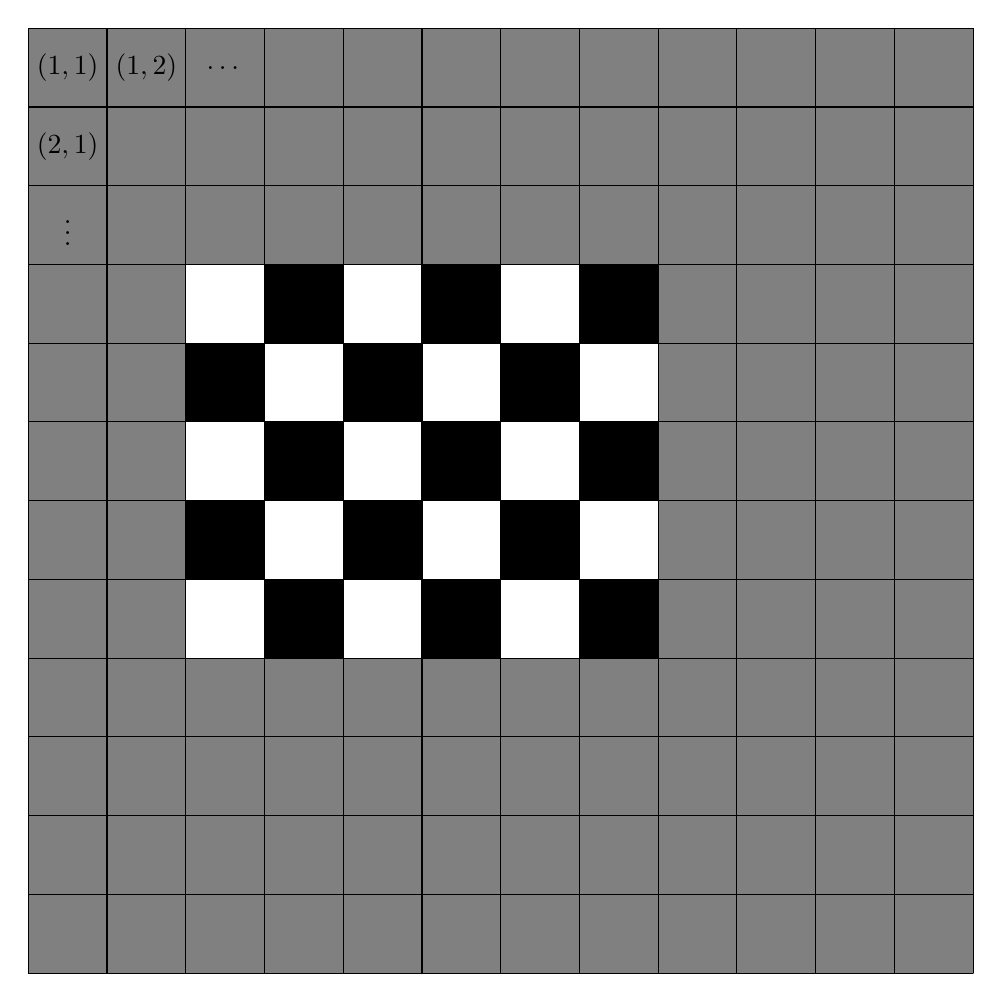
\begin{tikzpicture}
		\foreach \i in {-6, ..., 5}
			\foreach \j in {-6, ..., 5}
				\filldraw[gray] (\i, \j) rectangle + (1, 1);
		\foreach \i in {-4, ..., 1}
			\foreach \j in {-2, ..., 2}
			{
				\pgfmathparse{mod(\i+\j, 2) ? "black" : "white"}
				\edef\colour{\pgfmathresult}
				\filldraw[fill=\colour] (\i, \j) rectangle + (1, 1);
			}
		\draw[step=1] (-6, -6) grid (6, 6);
		\node at (-5.5, 5.5) {$(1, 1)$};
		\node at (-4.5, 5.5) {$(1, 2)$};
		\node at (-3.5, 5.5) {$\dots$};
		\node at (-5.5, 4.5) {$(2, 1)$};
		\node at (-5.5, 3.5) {$\vdots$};
	\end{tikzpicture}
	\caption{Example of a matrix, that contains a rROI with a checkerboard pattern. The top left corner of the rROI is $(4, 3)$ and the bottom right corner is $(8, 8)$. Here we have $m = n = 12$.}
	\label{fig: rROI}
\end{figure}

\paragraph{The statistical model}

Let $m, n \in \mathbb{N}$ and $c \in \mathbb{R} \setminus \{ 0 \}$. We assume a noisy image following the statistical model
\begin{equation}\label{statmodel}
	F(i, j) = \underbrace{c + V(i, j)}_{\eqqcolon \tilde{V}(i, j)} + \varepsilon_{i, j}
\end{equation}
for all $(i, j) \in \Omega \coloneqq \left\{ 1, \dots, m \right\} \times \left\{ 1, \dots, n \right\}$. The values of $V$ alternate between $c$ and $-c$ along the rows and columns of the region of interest, and call the set of all such images $\mathcal{V}_c^{m, n}$. The noise terms $\varepsilon_{i, j} \sim \mathcal{N}(0, \sigma^2)$ are assumed to be i.i.d. normally distributed random variables for some $\sigma > 0$.

For visualization we use grayscale images and set $c = 127.5$. Then the values of the image $\tilde{V}$ alternate between black and white within the region of interest. This gives the region of interest of $\tilde{V}$ a classical checkerboard pattern, see Figure \ref{fig: rROI} for an example.

Notably, we make two simplifications in our statistical model. First, we assume the variance $\sigma$ of the noise terms to be known beforehand. Second, we ignore the limitations of grayscale images and let the images in our model take all values in the real numbers. When trying to restore a ROI from an actual grayscale fingerprint image, the image, and thus the observed data $F$, would only take values in $\{ 0, \dots, 255 \}$.

The goal is to develop a statistical test for every pixel to determine whether or not the pixel belongs to the region of interest of $V$ and as such reconstructing the unknown $V$ from the noisy data. By choosing a checkerboard pattern, the discrete derivative operators can be employed to this end. The pixel $(i, j)$ belonging to the ROI is equivalent to $\min \{ \norm{\Delta^+ V(i, j)}, \norm{\Delta^- V(i, j)} \} \neq 0$, where $\Delta^+$ and $\Delta^-$ denote the forward and backward discrete derivative operator, respectively. Thus, we get the null and alternative hypotheses
\begin{align*}
	H_0(i, j)&: \min \{ \norm{\Delta^+ V(i, j)}, \norm{\Delta^- V(i, j)} \} = 0, \\
	H_1(i, j)&: \min \{ \norm{\Delta^+ V(i, j)}, \norm{\Delta^- V(i, j)} \} \neq 0.
\end{align*}
We use
\begin{equation*}
	T(i, j) \coloneqq \min \{ \norm{\Delta^+ F(i, j)}, \norm{\Delta^- F(i, j)} \}
\end{equation*}
as a test statistic for each pixel $(i, j) \in \Omega$. In the following, we denote by $\mathbb{P}_V( \ldots )$ the probability of an event given a \emph{fixed} image $V$.

If the null hypothesis $H_0(i, j)$ is true, we have $\norm{\Delta^+ V(i, j)} = 0$ or $\norm{\Delta^- V(i, j)} = 0$.

For $\norm{\Delta^+ V(i, j)} = 0$ we can bound the probability of a type I error by
\begin{equation*}
	\mathbb{P}_V( T(i, j) \geq t ) \leq \mathbb{P}_V( \norm{\Delta^+ F(i, j)} \geq t )
\end{equation*}
and for $\norm{\Delta^- V(i, j)} = 0$ by
\begin{equation*}
	\mathbb{P}_V( T(i, j) \geq t ) \leq \mathbb{P}_V( \norm{\Delta^- F(i, j)} \geq t ).
\end{equation*}

The right hand side of both inequalities is the same function, which can be computed explicitly. Using a trial and error algorithm, we can find a threshold $t_\alpha$ for a given statistical significance $\alpha \in ( 0, 1 )$, such that
\begin{equation*}
	\mathbb{P}_V( T(i, j) \geq t_\alpha ) \leq \alpha
\end{equation*}
for every $(i, j) \in \Omega$, if $H_0(i, j)$ is true. Since this is independent of the specific $V$, it holds for all images $V$ under which the null hypothesis for the pixel $(i, j)$ is true and thus we can bound the probability of falsely categorizing a background pixel as a foreground pixel by a given statistical significance $\alpha \in ( 0, 1 )$.

\paragraph{Main results}

We aim at researching the changes of the upper bounds of the error probabilities under morphological opening and closing.

Let $\mathfrak{I} \in \{ 0, 1 \}^{m \times n}$ be a binary matrix and $\Psi \subseteq \mathbb{Z}^2$ be a \emph{structuring element}, see \cite{imageprocessing}, we denote by $\mathfrak{I} \circ \Psi$ the opening of the binary matrix $\mathfrak{I}$ by $\Psi$ and by $\mathfrak{I} \bullet \Psi$ the closing of the binary matrix $\mathfrak{I}$ by $\Psi$.

As the region of interest in our case is rectangular, we use a square structuring element. We show, that using such a square structuring element yields an exponential improvement of the upper bound of the probability of a type I error after morphological opening compared to the upper bound before opening is applied. Applying morphological closing after opening will worsen this bound, but only polynomially. Overall, we obtain a better upper bound for the probability of a type I error, when applying morphological opening and closing. This allows us to lower the threshold $t_\alpha$ in the statistical test, potentially increasing the number of type I errors. Through the improvement of the upper bound, we can still bound the probability of a type I error after morphological opening and closing below a given statistical significance $\alpha$. The following theorem formalizes the change of the upper bounds.

\begin{theorem}
	Let $\Omega = \left\{ 1, \dots, m \right\} \times \left\{ 1, \dots, m \right\}$. Assume $F$ follows the statistical model given in \eqref{statmodel}.
	
	For a statistical significance $\alpha \in (0, 1)$, let $t_\alpha$ be a threshold, such that $\mathbb{P}_V( \norm{\Delta^+ F(\tilde{i}, \tilde{j})} \geq t_\alpha ) \leq \alpha$, if $\norm{\Delta^+ V(\tilde{i}, \tilde{j})} = 0$, and $\mathbb{P}_V( \norm{\Delta^- F(\tilde{i}, \tilde{j})} \geq t_\alpha ) \leq \alpha$, if $\norm{\Delta^- V(\tilde{i}, \tilde{j})} = 0$, for every $\tilde{i}, \tilde{j} \in \Omega$.
	
	Let $\mathfrak{I}_\alpha$ be the binary image defined by
	\begin{equation*}
	\mathfrak{I}_\alpha(\tilde{i}, \tilde{j}) = \mathds{1}_{ \{ T(\tilde{i}, \tilde{j}) \geq t_\alpha \} }
	\end{equation*}
	for all $(\tilde{i}, \tilde{j}) \in \Omega$.
	
	Let $\varphi \in \mathbb{N}$ be odd and define the set $\Phi_\varphi = \left\{ -\frac{\varphi - 1}{2}, -\frac{\varphi - 3}{2}, \dots, \frac{\varphi - 3}{2}, \frac{\varphi - 1}{2} \right\}$ and the structuring element $\Psi_\varphi = \Phi_\varphi \times \Phi_\varphi$.
	
	Then for $(i, j) \in \Omega$ the following inequalities hold, if $H_0(i, j)$ is true:
	\begin{align}
		\mathbb{P}_V\left( (\mathfrak{I}_\alpha \circ \Psi_\varphi)(i, j) = 1 \right) &\leq \varphi \alpha^{\frac{\varphi + 1}{2}} \label{ineq: introtypeIopening} \\
		\mathbb{P}_V\left( ((\mathfrak{I}_\alpha \circ \Psi_\varphi) \bullet \Psi_\varphi)(i, j) = 1 \right) &\leq \varphi^3 \alpha^{\frac{\varphi + 1}{2}} \label{ineq: introtypeIclosing}
	\end{align}
\end{theorem}

The question of bounding the probability of a type II error after morphological opening and closing also arises. It turns out, morphological opening increases the upper bound of this probability polynomially. The application of morphological closing, when applied after opening, does not improve the upper bound, since independence of the pixels is not guaranteed anymore. This is formalized in the following theorem.

\begin{theorem}
	Let $\Omega = \left\{ 1, \dots, m \right\} \times \left\{ 1, \dots, m \right\}$. Assume $F$ follows the statistical model given in \eqref{statmodel}.
	
	Let $t$ be a threshold, such that
	\begin{equation*}
		\mathbb{P}_V\left( T(\tilde{i}, \tilde{j}) \leq t \right) \leq \beta
	\end{equation*}
	for some $\beta \in (0, 1)$, all $(\tilde{i}, \tilde{j}) \in \Omega$ and all $V$, such that $H_1(\tilde{i}, \tilde{j})$ is true.
	
	Let $\mathfrak{I}$ be the binary image defined by
	\begin{equation*}
		\mathfrak{I}(\tilde{i}, \tilde{j}) = \mathds{1}_{ \{ T(\tilde{i}, \tilde{j}) \geq t \} }
	\end{equation*}
	for all $(\tilde{i}, \tilde{j}) \in \Omega$.
	
	Let $\varphi \in \mathbb{N}$ be odd and define the set $\Phi_\varphi = \left\{ -\frac{\varphi - 1}{2}, -\frac{\varphi - 3}{2}, \dots, \frac{\varphi - 3}{2}, \frac{\varphi - 1}{2} \right\}$ and the structuring element $\Psi_\varphi = \Phi_\varphi \times \Phi_\varphi$.
	
	Let $(i, j) \in \Omega$ and $V \in \mathcal{H}_1(i, j)$.
	
	Assume, that the rectangular region of interest contained in $V$ has side lengths larger than $\varphi$.
	
	Then for $(i, j) \in \Omega$ the following inequalities hold, if $H_1(i, j)$ is true:
	\begin{align}
		\mathbb{P}_V\left( (\mathfrak{I} \circ \Psi_\varphi)(i, j) = 0 \right) &\leq \varphi^2 \beta \label{ineq: introtypeIIopening} \\
		\mathbb{P}_V\left( ((\mathfrak{I} \circ \Psi_\varphi) \bullet \Psi_\varphi)(i, j) = 0 \right) &\leq \varphi^2 \beta \label{ineq: introtypeIIclosing}
	\end{align}
\end{theorem}

Note, that the bounds in the previous theorems are independent of the specific $(i, j)$. This means, that the bounds also hold for the worst case, i.e. pixels directly at the transition from background to foreground.

We simulate six different positions of $(i, j)$ with respect to the region of interest, see Figure \ref{fig: simulatedpixeltypes}. Regardless of the position of the pixel, morphological opening decreases the rate of type I errors as expected from inequality \eqref{ineq: introtypeIopening}. The increase of this rate through morphological closing, suggested by inequality \eqref{ineq: introtypeIclosing}, can not be observed. On the other hand, the rate of type II errors does not increase under morphological opening as much as inequality \eqref{ineq: introtypeIIopening} suggests. The fact, that the upper bound in inequalities \eqref{ineq: introtypeIIopening} and \eqref{ineq: introtypeIIclosing} is the same is well reflected in the simulation results.

\paragraph{Outlook}

The region of interest in this simplified model is convex and has an oscillatory pattern, similar to a fingerprint image. We used the discrete derivative operator to binarize the image and proceeded by applying morphological opening and closing.

The results presented in this thesis do not simply carry over to fingerprints. How the error probabilities can be bounded as well as how a structuring element should be chosen are questions that need to be explored.

Furthermore, we only considered bounds for single pixels. A next step should involve methods from the field of multiple testing to consider the simultaneous test of all pixels in the image.

\paragraph{Outline of the thesis}

In Section \ref{section: definitions} we introduce definitions and notation of the aforementioned images and properties. With the introduced terminology we develop a statistical test for every pixel determining whether or not it is part of the region of interest in Section \ref{section: statisticalmodel}. After having established the statistical test, we proof in Section \ref{section: boundtypeIerror} that we can bound the probability of a type I error by a given statistical significance and analyze the probability of a type II error in the statistical test in Section \ref{section: analyzetypeIIerror}. In Section \ref{section: morphologicaloperations} the two morphological operators, that we study in this thesis, are introduced, along with some examples of their application. From there, we proceed to proof the main theorems of this thesis in Section \ref{section: mainresults}. We compare our theoretical results to simulations in Section \ref{section: simulationresults} and discuss possible further research in Section \ref{section: conclusion}.

\newpage



\section{Testing for a rectangular region of interest}

\subsection{Definitions}\label{section: definitions}

Assume that the noise-free image $V$ in our statistical model has a rectangular region of interest with a checkerboard pattern, cf. equation \eqref{statmodel} and Figure \ref{fig: rROI}. In the following we give formal definitions of these properties.

\begin{definition}\label{def: rROIcheckerboard}
	Let $m, n \in \mathbb{N}$, $c \in \mathbb{R} \setminus \{ 0 \}$ and $V \in \{ 0, \pm c \}^{m \times n}$. We say that $V$ contains a \emph{rectangular region of interest with a checkerboard pattern}, if
	\begin{equation}
		V(i, j) =
		\begin{cases}
			c, \textrm{ if } (i, j) \in \{ \kappa_1, \dots, \kappa_2 \} \times \{ \lambda_1, \dots, \lambda_2 \} \textrm{ and } i + j \equiv \kappa_1 + \lambda_1 \mod 2 \\
			-c, \textrm{ if } (i, j) \in \{ \kappa_1, \dots, \kappa_2 \} \times \{ \lambda_1, \dots, \lambda_2 \} \textrm{ and } i + j \not\equiv \kappa_1 + \lambda_1 \mod 2 \\
			0, \textrm{ if } (i, j) \notin \{ \kappa_1, \dots, \kappa_2 \} \times \{ \lambda_1, \dots, \lambda_2 \}
		\end{cases}
	\end{equation}
	for some $(\kappa_1, \lambda_1), (\kappa_2, \lambda_2) \in \mathbb{N}^2$ with $1 \leq \kappa_1 \leq \kappa_2 \leq m$ and $1 \leq \lambda_1 \leq \lambda_2 \leq m$ and all $(i, j) \in \{ 1, \dots, m \} \times \{ 1, \dots, n \}$. The set of all such $V$ is denoted by $\mathcal{V}_c^{m, n}$.
	
	We call $\varLambda = \{ \kappa_1, \dots, \kappa_2 \} \times \{ \lambda_1, \dots, \lambda_2 \}$ a \emph{rectangular region of interest (rROI)} and say that $V$ contains the rROI $\varLambda$.
	
	Furthermore, we call $(\kappa_1, \lambda_1)$ the \emph{top left corner} and $(\kappa_2, \lambda_2)$ the \emph{bottom right corner} of $\varLambda$.
\end{definition}

Hence, the top left corner of the region of interest of $V$ takes the value $c$ and then the values of $V$ alternate between $+c$ and $-c$ along the rows and columns of the region of interest. This is similar to the classical checkerboard pattern.

\begin{remark}
	Any matrix $V \in \mathcal{V}_c^{m, n}$ is uniquely defined by the top left and bottom right corner of $\varLambda$. Hence, a rROI $\varLambda = \{ \kappa_1, \dots, \kappa_2 \} \times \{ \lambda_1, \dots, \lambda_2 \}$ corresponds to a unique element $V \in \mathcal{V}_c^{m, n}$, that contains the rROI $\varLambda$.
\end{remark}

\begin{remark}
	To adjust to boundary issues, we use a periodic boundary condition, i.e. we extend $V$ to all of $\mathbb{Z}^2$ by setting $V(i, j) = V(i \mod m, j \mod n)$ for all $(i, j) \in \mathbb{Z}^2$.
\end{remark}

In Figure \ref{fig: rROI} we see an example of such a matrix. To visualize these types of matrices, we take $c = 127.5$ and plot the grayscale image $V + c$. Thus, gray pixels represent $V = 0$, white pixels represent $V = c$ and black pixels represent $V = - c$.

We also need the forward and backward discrete derivative operator, whose definitions we give below, to establish our statistical test.

\begin{definition}
	Let $m, n \in \mathbb{N}$ and let $V \in \mathbb{R}^{m \times n}$. Define the set of possible indices $\Omega \coloneqq \{ 1, \dots, m \} \times \{ 1, \dots, m \}$. Let $(i, j) \in \Omega$. The \textit{forward and backward discrete derivative of $V$ evaluated at $(i, j)$} are defined as
	\begin{equation}
		\Delta^+ V(i, j) =
		\begin{pmatrix}
			V(i + 1, j) - V(i, j) \\
			V(i, j + 1) - V(i, j)
		\end{pmatrix}
	\end{equation}
	and
	\begin{equation}
		\Delta^- V(i, j) =
		\begin{pmatrix}
			V(i - 1, j) - V(i, j) \\
			V(i, j - 1) - V(i, j)
		\end{pmatrix}
		,
	\end{equation}
	respectively.
\end{definition}

The following lemma shows, that the euclidean norm of these operators evaluated at a pixel $(i, j) \in \Omega$ for matrices $V \in \mathcal{V}_c^{m, n}$ can only take specific values.

\begin{lemma}\label{lem: setD}
	Let $m, n \in \mathbb{N}$ and $c \in \mathbb{R} \setminus \{ 0 \}$. Let $V \in \mathcal{V}_c^{m, n}$. For any $(i, j) \in \Omega$ we have
	\begin{equation}
		\norm{\Delta^+ V(i, j)}, \norm{\Delta^- V(i, j)} \in \{ 0, c, \sqrt{2} c, \sqrt{5} c, \sqrt{8} c \}.
	\end{equation}
\end{lemma}
\begin{proof}
	Let $(i, j) \in \Omega$. We have assumed, that $V \in \mathcal{V}_c^{m, n}$. Thus, $V$ only takes values in $\{ 0, \pm c \}$ and we obtain $\Delta^+ V(i, j), \Delta^- V(i, j) \in \{ 0, \pm c, \pm 2 c \}^2$. Taking the euclidean norm of all possible combinations yields
	\begin{equation*}
		\norm{\Delta^+ V(i, j)}, \norm{\Delta^- V(i, j)} \in \{ 0, c, 2 c, \sqrt{2} c, \sqrt{5} c, \sqrt{8} c \}.
	\end{equation*}
	
	We can narrow this list down even more. By assumption, $V$ contains a rectangular region of interest $\varLambda$ with a checkerboard pattern. This only allows for the combinations of $\abs{V(i + 1, j) - V(i, j)}$ and $\abs{V(i, j + 1) - V(i, j)}$ listed in Table \ref{table: discretederivativevalues}.
	\begin{table}[t]
		\centering
		\resizebox{\textwidth}{!}{
			\begin{tabular}{c|c|c|c}
				\textbf{Position of pixels} $\mathbf{(i, j)}$, $\mathbf{(i + 1, j)}$, $\mathbf{(i, j + 1)}$ & $\mathbf{\abs{V(i + 1, j) - V(i, j)}}$ & $\mathbf{\abs{V(i, j + 1) - V(i, j)}}$ & $\mathbf{\norm{\Delta^+ V(i, j)}}$ \\
				\hline
				$(i, j), (i + 1, j), (i, j + 1) \notin \varLambda$ & $0$ & $0$ & $0$ \\
				\hline
				$(i, j), (i + 1, j) \notin \varLambda$ and $(i, j + 1) \in \varLambda$ & $0$ & $c$ & $c$ \\
				\hline
				$(i, j), (i, j + 1) \notin \varLambda$ and $(i + 1, j) \in \varLambda$ & $c$ & $0$ & $c$ \\
				\hline
				$(i, j) \in \varLambda$ and $(i + 1, j), (i, j + 1) \notin \varLambda$ & $c$ & $c$ & $\sqrt{2} c$ \\
				\hline
				$(i, j), (i + 1, j) \in \varLambda$ and $(i, j + 1) \notin \varLambda$ & $2 c$ & $c$ & $\sqrt{5} c$ \\
				\hline
				$(i, j), (i, j + 1) \in \varLambda$ and $(i + 1, j) \notin \varLambda$ & $c$ & $2 c$ & $\sqrt{5} c$ \\
				\hline
				$(i, j), (i + 1, j), (i, j + 1) \in \varLambda$ & $2 c$ & $2 c$ & $\sqrt{8} c$ \\
			\end{tabular}
		}
	\caption{Possible locations of the pixels $(i, j)$, $(i + 1, j)$, $(i, j + 1)$ and the corresponding values of $\abs{V(i + 1, j) - V(i, j)}$, $\abs{V(i, j + 1) - V(i, j)}$ and $\norm{\Delta^+ V(i, j)}$, respectively.}
	\label{table: discretederivativevalues}
	\end{table}
	
	Other cases are not possible and thus $\norm{\Delta^+ V(i, j)} \in \{ 0, c, \sqrt{2} c, \sqrt{5} c, \sqrt{8} c \}$. By analogous deduction, we also obtain $\norm{\Delta^- V(i, j)} \in \{ 0, c, \sqrt{2} c, \sqrt{5} c, \sqrt{8} c \}$.
\end{proof}



\subsection{Statistical model}\label{section: statisticalmodel}

Let $m, n \in \mathbb{N}$, $c \in \mathbb{R} \setminus \{ 0 \}$ and $\Omega = \left\{ 1, \dots, m \right\} \times \left\{ 1, \dots, n \right\}$. Assume we are given noisy data
\begin{equation}\label{statmodel2}
	F(i, j) = c + V(i, j) + \varepsilon_{i, j}
\end{equation}
for all $(i, j) \in \Omega$, where $V \in \mathcal{V}_c^{m, n}$ is unknown and $\varepsilon_{i, j} \sim \mathcal{N}(0, \sigma^2)$ are i.i.d. normal distributed random variables for some $\sigma > 0$.

Let $\varLambda$ be the rectangular region of interest contained in $V$. In the following we specify a statistical test to determine for each individual pixel whether $(i, j) \in \varLambda$ or $(i, j) \notin \varLambda$.

By the assumption, that $V$ contains a rROI, it follows, that $V(i, j) = 0$ if and only if $(i, j) \notin \varLambda$. Let $(\kappa_1, \lambda_1)$ and $(\kappa_2, \lambda_2)$ be the top left and bottom right corner of $\varLambda$, respectively. Now, if $(i, j) \notin \varLambda$, it follows that $i \notin \{ \kappa_1, \dots, \kappa_2 \}$ or $j \notin \{ \lambda_1, \dots, \lambda_2 \}$. We have to distinguish four cases here:
\begin{enumerate}[(I)]
	\item $\begin{aligned}[t]
		\hspace{40pt} i < \kappa_1 &\Rightarrow (i, j - 1) \notin \varLambda \textrm{ and } (i - 1, j) \notin \varLambda \\
		&\Rightarrow V(i, j - 1) = V(i - 1, j) = 0
	\end{aligned}$
	\item $\begin{aligned}[t]
		\hspace{40pt} j < \lambda_1 &\Rightarrow (i - 1, j) \notin \varLambda \textrm{ and } (i, j - 1) \notin \varLambda \\
		&\Rightarrow V(i - 1, j) = V(i, j - 1) = 0
	\end{aligned}$
	\item $\begin{aligned}[t]
		\hspace{40pt} i > \kappa_2 &\Rightarrow (i, j + 1) \notin \varLambda \textrm{ and } (i + 1, j) \notin \varLambda \\
		&\Rightarrow V(i, j + 1) = V(i + 1, j) = 0
	\end{aligned}$
	\item $\begin{aligned}[t]
		\hspace{40pt} j > \lambda_2 &\Rightarrow (i + 1, j) \notin \varLambda \textrm{ and } (i, j + 1) \notin \varLambda \\
		&\Rightarrow V(i + 1, j) = V(i, j + 1) = 0
	\end{aligned}$
\end{enumerate}

We have $\norm{\Delta^- V(i, j)} = 0$ in the first two cases and $\norm{\Delta^+ V(i, j)} = 0$ in the latter two cases. Thus, $(i, j) \notin \varLambda$ implies $\min \{ \norm{\Delta^+ V(i, j)}, \norm{\Delta^- V(i, j)} \} = 0$.

On the other hand, we have assumed, that $\varLambda$ has a checkerboard pattern. Thus $\norm{\Delta^- V(i, j)}, \norm{\Delta^+ V(i, j)} \neq 0$ for $(i, j) \in \varLambda$. This yields the equivalence
\begin{equation*}
	(i, j) \notin \varLambda \Leftrightarrow \min \{ \norm{\Delta^+ V(i, j)}, \norm{\Delta^- V(i, j)} \} = 0.
\end{equation*}

Using this equivalence, we test for each individual pixel $(i, j)$ the null hypothesis
\begin{equation}\label{nullhypothesis}
	H_0(i, j): \min \{ \norm{\Delta^+ V(i, j)}, \norm{\Delta^- V(i, j)} \} = 0
\end{equation}
against the alternative hypothesis
\begin{equation}\label{alternativehypothesis}
	H_1(i, j): \min \{ \norm{\Delta^+ V(i, j)}, \norm{\Delta^- V(i, j)} \} \neq 0
\end{equation}
using the test statistic
\begin{equation}\label{teststatistic}
	T(i, j) \coloneqq \min \{ \norm{\Delta^+ F(i, j)}, \norm{\Delta^- F(i, j)} \},
\end{equation}
which is based on the given noisy data.

To extract the rROI, we classify pixels as foreground, if we reject the null hypothesis, i.e. if $T(i, j) \geq t$ for some threshold $t \in \mathbb{R}^+$. The choice of the threshold is examined in Section \ref{section: boundtypeIerror}.

For convenience, we want to define some subsets of $\mathcal{V}_c^{m, n}$. For every $(i, j) \in \Omega$ we define the set of images, for which the null hypothesis $H_0(i, j)$ is true as
\begin{equation}
	\mathcal{H}_0(i, j) \coloneqq \left\{ V \in \mathcal{V}_c^{m, n} \mid \min \{ \norm{\Delta^+ V(i, j)}, \norm{\Delta^- V(i, j)} \} = 0 \right\}.
\end{equation}

Then $H_0(i, j)$ is true, if and only if $V \in \mathcal{H}_0(i, j)$. Furthermore, we define two subsets of this set as
\begin{align}
	\mathcal{H}_0^+(i, j) &\coloneqq \left\{ V \in \mathcal{V}_c^{m, n} \mid \norm{\Delta^+ V(i, j)} = 0 \right\} \label{setH0+}, \\
	\mathcal{H}_0^-(i, j) &\coloneqq \left\{ V \in \mathcal{V}_c^{m, n} \mid \norm{\Delta^- V(i, j)} = 0 \right\} \label{setH0-}.
\end{align}

Then $\mathcal{H}_0(i, j) = \mathcal{H}_0^+(i, j) \cup \mathcal{H}_0^-(i, j)$, where the union is not necessarily disjoint.



\subsection{Bound for the probability of a type I error}\label{section: boundtypeIerror}

Having established our hypotheses and test statistic, we want to examine the choice of the threshold $t \in \mathbb{R}^+$ in the testing procedure. We reject the null hypothesis, if $T(i, j) \geq t$ for some threshold $t \in \mathbb{R}^+$. We want to choose $t$ such, that the probability of falsely classifying a background pixel as foreground is bounded from above by a given statistical significance $\alpha \in (0, 1)$. Such a threshold will be denoted as $t_\alpha$.

As a reminder, we use the notation $\mathbb{P}_V( \ldots )$ for the probability of an event for some \emph{fixed} image $V$. This will allow us to analyze the probabilites of falsely categorizing a pixel. Using this notation, we want to find a threshold $t_\alpha$, such that $\mathbb{P}_V( T(i, j) \geq t_\alpha ) \leq \alpha$ for every $V \in \mathcal{H}_0(i, j)$. A first step towards finding such a threshold is the following lemma.

\begin{lemma}\label{lem: typeIbound}
	Let $(i, j) \in \Omega$ and $t \in \mathbb{R}^+$. Assume that $F$ follows the statistical model given in \eqref{statmodel2} and let $T(i, j)$ be defined as in \eqref{teststatistic}. Let $V \in \mathcal{V}_c^{m, n}$. Then
	\begin{equation}
		\mathbb{P}_V( T(i, j) \geq t ) \leq \min \left\{ \mathbb{P}_V( \norm{\Delta^+ F(i, j)} \geq t ), \mathbb{P}_V( \norm{\Delta^- F(i, j)} \geq t ) \right\}.
	\end{equation}
\end{lemma}
\begin{proof}
	Let $t \in \mathbb{R}^+$. We have
	\begin{align*}
		\mathbb{P}_V( T(i, j) \geq t ) &= \mathbb{P}_V( \min \{ \norm{\Delta^+ F(i, j)}, \norm{\Delta^- F(i, j)} \} \geq t ) \\
		&= \mathbb{P}_V( \{ \norm{\Delta^+ F(i, j)} \geq t \} \cap \{ \norm{\Delta^- F(i, j)} \geq t \} ) \\
		&\leq \mathbb{P}_V( \norm{\Delta^+ F(i, j)} \geq t ).
	\end{align*}
	
	Analogously, we obtain
	\begin{equation*}
		\mathbb{P}_V( T(i, j) \geq t ) \leq \mathbb{P}_V( \norm{\Delta^- F(i, j)} \geq t ).
	\end{equation*}
	
	Combining these two inequalities yields the result and thus finishes the proof of the lemma.
\end{proof}

The second step is given in the following theorem, where we calculate the cumulative distribution functions of $\mathbb{P}_V( \norm{\Delta^+ F(i, j)} \leq t )$ for $V \in \mathcal{H}_0^+(i, j)$ and $\mathbb{P}_V( \norm{\Delta^- F(i, j)} \leq t )$ for $V \in \mathcal{H}_0^-(i, j)$, which turn out to be the same.

\begin{theorem}\label{thm: cdf}
	Let $(i, j) \in \Omega$ and $t \in \mathbb{R}^+$. Assume that $F$ follows the statistical model given in \eqref{statmodel2}. Let $V_1 \in \mathcal{H}_0^+(i, j)$ and $V_2 \in \mathcal{H}_0^-(i, j)$. Then
	\begin{equation}\label{eq: probequality}
		\mathbb{P}_{V_1}( \norm{\Delta^+ F(i, j)} \leq t ) = p_\sigma(t) = \mathbb{P}_{V_2}( \norm{\Delta^- F(i, j)} \leq t )
	\end{equation}
	where
	\begin{equation}\label{eq: cdf}
		\begin{aligned}
			p_\sigma(t) &\coloneqq \frac{1}{\sqrt{3}} \left( \frac{3}{2} - \frac{3}{2} \exp \left( - \frac{t^2}{3 \sigma^2} \right) I_0 \left( \frac{t^2}{6 \sigma^2} \right) \right) - \sqrt{3} \\
			&\quad - \frac{2 - \sqrt{3}}{2} Q_1 \left( \sqrt{\frac{2 - \sqrt{3}}{6}} \frac{t}{\sigma}, \sqrt{\frac{2 + \sqrt{3}}{6}} \frac{t}{\sigma} \right) \\
			&\quad + \frac{2 + \sqrt{3}}{2} Q_1 \left( \sqrt{\frac{2 + \sqrt{3}}{6}} \frac{t}{\sigma}, \sqrt{\frac{2 - \sqrt{3}}{6}} \frac{t}{\sigma} \right)
		\end{aligned}
	\end{equation}
	with $I_0$ being the modified Bessel function of the first kind \cite[p.~910-911]{TISP} and $Q_M$ denoting the Marcum $Q$-function \cite{IntQFunction}.
\end{theorem}
\begin{proof}
	We start by proving the first equality of equation \eqref{eq: probequality}. By assumption, $V_1 \in \mathcal{H}_0^+(i, j)$ and thus $\norm{\Delta^+ V_1(i, j)} = 0$. By definition of $\Delta^+$ we get the equivalence
	\begin{equation*}
		\norm{\Delta^+ V_1(i, j)} = 0 \Leftrightarrow V_1(i + 1, j) - V_1(i, j) = V_1(i, j + 1) - V_1(i, j) = 0.
	\end{equation*}
	
	We write out the term $\mathbb{P}_{V_1}( \norm{\Delta^+ F(i, j)} \leq t )$, which we call $q(t)$, and use the equivalence above to obtain
	\begin{align*}
		q(t) &\coloneqq \mathbb{P}_{V_1}( \norm{\Delta^+ F(i, j)} \leq t ) \\
		&= \mathbb{P}_{V_1}\big( (c + V_1(i + 1, j) + \varepsilon_{i + 1, j} - c - V_1(i, j) - \varepsilon_{i, j})^2 \\
		&\quad + (c + V_1(i, j + 1) + \varepsilon_{i, j + 1} - c - V_1(i, j) - \varepsilon_{i, j})^2 \leq t^2 \big) \\
		&= \mathbb{P}_{V_1}\left( (\varepsilon_{i + 1, j} - \varepsilon_{i, j})^2 + (\varepsilon_{i, j + 1} - \varepsilon_{i, j})^2 \leq t^2 \right) \\
		&= \mathbb{P}\left( (\varepsilon_{i + 1, j} - \varepsilon_{i, j})^2 + (\varepsilon_{i, j + 1} - \varepsilon_{i, j})^2 \leq t^2 \right) \\
		&= \mathbb{P}\left( \sqrt{(\varepsilon_{i + 1, j} - \varepsilon_{i, j})^2 + (\varepsilon_{i, j + 1} - \varepsilon_{i, j})^2} \leq t \right)
	\end{align*}
	where we dropped the index $V_1$, since the probability does no longer depend on the chosen $V_1$.
	
	To proceed, we need to determine the distribution of the random variable $\sqrt{(\varepsilon_{i + 1, j} - \varepsilon_{i, j})^2 + (\varepsilon_{i, j + 1} - \varepsilon_{i, j})^2}$ conditioned on $\varepsilon_{i, j} = \epsilon$ for some fixed $\epsilon \in \mathbb{R}$.
	
	We define the random variables
	\begin{align*}
		X_1 &= \varepsilon_{i + 1, j} - \epsilon \sim \mathcal{N}(- \epsilon, \sigma^2), \\
		X_2 &= \varepsilon_{i, j + 1} - \epsilon \sim \mathcal{N}(- \epsilon, \sigma^2)
	\end{align*}
	and obtain
	\begin{align*}
		&\mathbb{P}\left( \sqrt{(\varepsilon_{i + 1, j} - \varepsilon_{i, j})^2 + (\varepsilon_{i, j + 1} - \varepsilon_{i, j})^2} \leq t \mid \varepsilon_{i, j} = \epsilon \right) \\
		&= \mathbb{P}\left( \sqrt{(\varepsilon_{i + 1, j} - \epsilon)^2 + (\varepsilon_{i, j + 1} - \epsilon)^2} \leq t \right) \\
		&= \mathbb{P}\left( \sqrt{\left( \frac{X_1}{\sigma} \right)^2 + \left( \frac{X_2}{\sigma} \right)^2} \leq \frac{t}{\sigma} \right).
	\end{align*}
	
	Since $X_1$ and $X_2$ are independent, the square root inside has a non-central Chi distribution with two degrees of freedom and non-centrality parameter
	\begin{equation*}
		\lambda = \sqrt{\left( \frac{- \epsilon}{\sigma} \right)^2 + \left( \frac{- \epsilon}{\sigma} \right)^2} = \frac{\sqrt{2} \abs{\epsilon}}{\sigma}.
	\end{equation*}
	
	This yields
	\begin{equation*}
		\sqrt{\left( \frac{X_1}{\sigma} \right)^2 + \left( \frac{X_2}{\sigma} \right)^2} \sim \chi_2 \left( \frac{\sqrt{2} \abs{\epsilon}}{\sigma} \right)
	\end{equation*}
	and consequently
	\begin{equation*}
		\frac{\sqrt{(\varepsilon_{i + 1, j} - \varepsilon_{i, j})^2 + (\varepsilon_{i, j + 1} - \varepsilon_{i, j})^2}}{\sigma} \mid \varepsilon_{i, j} = \epsilon \sim \chi_2 \left( \frac{\sqrt{2} \abs{\epsilon}}{\sigma} \right).
	\end{equation*}
	
	Up to this point, we assumed $\varepsilon_{i, j}$ to be fixed, however it is itself a normal distributed random variable with zero mean and standard deviation $\sigma$. Thus, we have a compound probability distribution and obtain
	\begin{align*}
		q(t) &= \mathbb{P}\left( \frac{\sqrt{(\varepsilon_{i + 1, j} - \varepsilon_{i, j})^2 + (\varepsilon_{i, j + 1} - \varepsilon_{i, j})^2}}{\sigma} \leq \frac{t}{\sigma} \right) \\
		&= \int_0^\frac{t}{\sigma} \int_0^\infty \underbrace{x \exp \left( - \frac{x^2}{2} - \frac{\eta^2}{\sigma^2} \right) I_0 \left( \frac{\sqrt{2} \eta}{\sigma} x \right)}_{\textrm{pdf of} \ \chi_2 \left( \frac{\sqrt{2} \eta}{\sigma} \right) \ \textrm{for fixed} \ \eta} \underbrace{\frac{2}{\sqrt{2 \pi \sigma^2}} \exp \left( - \frac{\eta^2}{2 \sigma^2} \right)}_{\textrm{pdf of absolute value of} \ \mathcal{N}(0, \sigma^2)} \mathrm{d}\eta \mathrm{d}x \\
		&= \frac{2}{\sqrt{2 \pi \sigma^2}} \int_0^\frac{t}{\sigma} x \exp \left( - \frac{x^2}{2} \right) \int_0^\infty \exp \left( - \frac{3}{2 \sigma^2} \eta^2 \right) I_0 \left( \frac{\sqrt{2} x}{\sigma} \eta \right) \mathrm{d}\eta \mathrm{d}x,
	\end{align*}
	
	where $I_0$ is the modified Bessel function of the first kind. We can solve the inner integral first. For $\nu > -1$, $\alpha > 0$ the following equality holds.\footnote{\fullcite[p.~699]{TISP}}
	\begin{equation}\label{eq: intbessel}
		\int_0^\infty \exp \left( - \alpha \eta^2 \right) I_\nu ( \beta \eta ) \mathrm{d}\eta = \frac{\sqrt{\pi}}{2 \sqrt{\alpha}} \exp \left( \frac{\beta^2}{8 \alpha} \right) I_{\frac{1}{2} \nu} \left( \frac{\beta^2}{8 \alpha} \right)
	\end{equation}
	
	In our case, we have $\nu = 0 > -1$, $\alpha = \frac{3}{2 \sigma^2} > 0$ and $\beta = \frac{\sqrt{2} x}{\sigma}$, which yields
	\begin{align*}
		\int_0^\infty \exp \left( - \frac{3}{2 \sigma^2} \eta^2 \right) I_0 \left( \frac{\sqrt{2} x}{\sigma} \eta \right) \mathrm{d}\eta &= \frac{\sqrt{\pi}}{2 \sqrt{\frac{3}{2 \sigma^2}}} \exp \left( \frac{\frac{2 x^2}{\sigma^2}}{8 \frac{3}{2 \sigma^2}} \right) I_0 \left( \frac{\frac{2 x^2}{\sigma^2}}{8 \frac{3}{2 \sigma^2}} \right) \\
		&= \frac{\sqrt{\pi} \sigma}{\sqrt{6}} \exp \left( \frac{x^2}{6} \right) I_0 \left( \frac{x^2}{6} \right).
	\end{align*}
	
	Plugging this in, we obtain
	\begin{align*}
		q(t) &= \frac{2}{\sqrt{2 \pi \sigma^2}} \int_0^\frac{t}{\sigma} x \exp \left( - \frac{x^2}{2} \right) \frac{\sqrt{\pi} \sigma}{\sqrt{6}} \exp \left( \frac{x^2}{6} \right) I_0 \left( \frac{x^2}{6} \right) \mathrm{d}x \\
		&= \frac{1}{\sqrt{3}} \int_0^\frac{t}{\sigma} x \exp \left( - \frac{x^2}{2} \right) \exp \left( \frac{x^2}{6} \right) I_0 \left( \frac{x^2}{6} \right) \mathrm{d}x \\
		&= \frac{1}{\sqrt{3}} \int_0^\frac{t}{\sigma} x \exp \left( - \frac{x^2}{3} \right) I_0 \left( \frac{x^2}{6} \right) \mathrm{d}x.
	\end{align*}
	
	To proceed, we need to integrate by parts to replace the modified Bessel function $I_0$ with order zero by a modified Bessel function $I_1$ with order one.\footnote{\fullcite[p.~251]{HMF}}
	\begin{align*}
		q(t) &= \frac{1}{\sqrt{3}} \left[ - \frac{3}{2} \exp \left( - \frac{x^2}{3} \right) I_0 \left( \frac{x^2}{6} \right) \right]_0^\frac{t}{\sigma} + \frac{1}{2 \sqrt{3}} \int_0^\frac{t}{\sigma} \exp \left( - \frac{x^2}{3} \right) x I_1 \left( \frac{x^2}{6} \right) \mathrm{d}x \\
		&= \frac{1}{\sqrt{3}} \left( \frac{3}{2} - \frac{3}{2} \exp \left( - \frac{t^2}{3 \sigma^2} \right) I_0 \left( \frac{t^2}{6 \sigma^2} \right) \right) + \frac{1}{2 \sqrt{3}} \int_0^\frac{t}{\sigma} \exp \left( - \frac{x^2}{3} \right) x I_1 \left( \frac{x^2}{6} \right) \mathrm{d}x
	\end{align*}
	
	In the next step we substitute $y = x^2$ in the remaining integral, which leaves us with
	\begin{equation*}
		q(t) = \frac{1}{\sqrt{3}} \left( \frac{3}{2} - \frac{3}{2} \exp \left( - \frac{t^2}{3 \sigma^2} \right) I_0 \left( \frac{t^2}{6 \sigma^2} \right) \right) + \frac{1}{4 \sqrt{3}} \int_0^\frac{t^2}{\sigma^2} \exp \left( - \frac{y}{3} \right) I_1 \left( \frac{y}{6} \right) \mathrm{d}y.
	\end{equation*}
	
	We want to solve the remaining integral. Let $p \neq b$ and $s = \sqrt{p^2 - b^2}$, $u = \sqrt{a (p - s)}$ and $v = \sqrt{a (p + s)}$. Then\footnote{\fullcite{IntQFunction}}
	\begin{equation}\label{eq: intmarcum}
		\int_0^a \exp(-p x) I_M ( b x ) \mathrm{d}x = \frac{1}{s b^M} \left( (p - s)^M ( 1 - Q_M(u, v) ) - (p + s)^M ( 1 - Q_M(v, u) ) \right),
	\end{equation}
	where $Q_M$ denotes the Marcum $Q$-function. The Marcum $Q$-function is only defined for $M \geq 1$, which made the integration by parts necessary. Applying this equation with $M = 1$ to the integral yields
	\begin{align*}
		\int_0^\frac{t^2}{\sigma^2} \exp \left( - \frac{y}{3} \right) I_1 \left( \frac{y}{6} \right) \mathrm{d}y &= 2 \sqrt{3} (2 - \sqrt{3}) \left( 1 - Q_1 \left( \sqrt{\frac{2 - \sqrt{3}}{6}} \frac{t}{\sigma}, \sqrt{\frac{2 + \sqrt{3}}{6}} \frac{t}{\sigma} \right) \right) \\
		&\quad - 2 \sqrt{3} (2 + \sqrt{3}) \left( 1 - Q_1 \left( \sqrt{\frac{2 + \sqrt{3}}{6}} \frac{t}{\sigma}, \sqrt{\frac{2 - \sqrt{3}}{6}} \frac{t}{\sigma} \right) \right).
	\end{align*}
	
	Plugging this in, we obtain the final result
	\begin{align*}
		q(t) &= \frac{1}{\sqrt{3}} \left( \frac{3}{2} - \frac{3}{2} \exp \left( - \frac{t^2}{3 \sigma^2} \right) I_0 \left( \frac{t^2}{6 \sigma^2} \right) \right) + \frac{1}{4 \sqrt{3}} \int_0^\frac{t^2}{\sigma^2} \exp \left( - \frac{y}{3} \right) I_1 \left( \frac{y}{6} \right) \mathrm{d}y \\
		&= \frac{1}{\sqrt{3}} \left( \frac{3}{2} - \frac{3}{2} \exp \left( - \frac{t^2}{3 \sigma^2} \right) I_0 \left( \frac{t^2}{6 \sigma^2} \right) \right) \\
		&\quad + \frac{2 \sqrt{3}}{4 \sqrt{3}} (2 - \sqrt{3}) \left( 1 - Q_1 \left( \sqrt{\frac{2 - \sqrt{3}}{6}} \frac{t}{\sigma}, \sqrt{\frac{2 + \sqrt{3}}{6}} \frac{t}{\sigma} \right) \right) \\
		&\quad - \frac{2 \sqrt{3}}{4 \sqrt{3}} (2 + \sqrt{3}) \left( 1 - Q_1 \left( \sqrt{\frac{2 + \sqrt{3}}{6}} \frac{t}{\sigma}, \sqrt{\frac{2 - \sqrt{3}}{6}} \frac{t}{\sigma} \right) \right) \\
		&= \frac{1}{\sqrt{3}} \left( \frac{3}{2} - \frac{3}{2} \exp \left( - \frac{t^2}{3 \sigma^2} \right) I_0 \left( \frac{t^2}{6 \sigma^2} \right) \right) - \sqrt{3} \\
		&\quad - \frac{2 - \sqrt{3}}{2} Q_1 \left( \sqrt{\frac{2 - \sqrt{3}}{6}} \frac{t}{\sigma}, \sqrt{\frac{2 + \sqrt{3}}{6}} \frac{t}{\sigma} \right) \\
		&\quad + \frac{2 + \sqrt{3}}{2} Q_1 \left( \sqrt{\frac{2 + \sqrt{3}}{6}} \frac{t}{\sigma}, \sqrt{\frac{2 - \sqrt{3}}{6}} \frac{t}{\sigma} \right) \\
		&= p_\sigma(t).
	\end{align*}
	
	This finishes the proof of the first equality of equation \eqref{eq: cdf}. Analogously, we can proof $\mathbb{P}_{V_2}( \norm{\Delta^- F(i, j)} \leq t ) = p_\sigma(t)$, finishing the proof of Theorem~\ref{thm: cdf}.
\end{proof}

\begin{remark}
	The Marcum Q-function is defined as
	\begin{equation*}
		Q_M(a, b) = \int_b^\infty x \left( \frac{x}{a} \right)^{M-1} \exp \left( -\frac{x^2 + a^2}{2} \right) I_{M-1}(a x) \mathrm{d}x.
	\end{equation*}
	
	The cumulative distribution function of a non-central chi distributed random variable with $k$ degrees of freedom and non-centrality parameter $\lambda$ given by $1 - Q_\frac{k}{2}(\lambda, x)$.
\end{remark}

\begin{corollary}\label{cor: typeIbound}
	Let $(i, j) \in \Omega$ and $t \in \mathbb{R}^+$. Assume that $F$ follows the statistical model given in \eqref{statmodel2} and let $T(i, j)$ be defined as in \eqref{teststatistic}. Then
	\begin{equation}
		\mathbb{P}_V( T(i, j) \geq t ) \leq 1 - p_\sigma(t)
	\end{equation}
	for every $V \in \mathcal{H}_0(i, j)$.
\end{corollary}
\begin{proof}
	Since $V \in \mathcal{H}_0(i, j)$, we have $V \in \mathcal{H}_0^+(i, j)$ or $V \in \mathcal{H}_0^-(i, j)$. In the first case, by Lemma \ref{lem: typeIbound} and Theorem \ref{thm: cdf} we have
	\begin{align*}
		\mathbb{P}_V( T(i, j) \geq t ) &\leq \min \left\{ \mathbb{P}_V( \norm{\Delta^+ F(i, j)} \geq t ), \mathbb{P}_V( \norm{\Delta^- F(i, j)} \geq t ) \right\} \\
		&\leq \mathbb{P}_V( \norm{\Delta^+ F(i, j)} \geq t ) \\
		&= 1 - p_\sigma(t).
	\end{align*}
	
	The second case is proven analogously.
\end{proof}

Let $\alpha \in (0, 1)$ be given. According to Corollary \ref{cor: typeIbound} any threshold $t_\alpha$ with $1 - p_\sigma(t_\alpha) \leq \alpha$ bounds the probability of a type I error in our statistical test below the given statistical significance $\alpha$. Since the function $p_\sigma(t)$ does not depend on $V$, the threshold is independent of the specific $V$.

Note, that finding inverse functions of the modified Bessel function of the first kind $I_\nu$ and of the Marcum $Q$-function $Q_M$ is not feasible and consequently there is no way to compute an inverse function of $p_\sigma(t)$. Thus, we cannot provide a closed form to calculate the threshold, but we can compute a threshold $t_\alpha$ numerically with a trial and error algorithm, see Algorithm \ref{alg: threshold}.

To this end, we note, that $p_\sigma(t_\alpha \cdot \sigma) = p_1(t_\alpha)$. Hence, it is sufficient to calculate a threshold $t_\alpha$ for $\sigma = 1$. A \emph{MATLAB} implementation of this algorithm can be found in Appendix \ref{appendix: algorithms}. In Figure \ref{fig: cdf} the cumulative distribution function $p_1(t)$ is plotted. For $\alpha = 0.05$ and $\alpha = 0.01$ the thresholds have been numerically computed.\\

\begin{algorithm}[H]
	\KwIn{$\alpha \in (0, 1)$}
	\KwOut{$t_\alpha$ and $\alpha_{real}$, s.t. $p_1(t_\alpha) = 1 - \alpha_{real} \geq 1 - \alpha$}
	$t_\alpha = 0$\;
	$t_{inc} = 0.0001$\;
	\While{$p_1(t_\alpha) < 1 - \alpha$}
	{
		$t_\alpha + t_{inc}$\;
		$\alpha_{real} = 1 - p_1(t_\alpha)$\;
	}
	\caption{Computation of a threshold for a given statistical significance}
	\label{alg: threshold}
\end{algorithm}

% Plot cumulative distribution function:
\begin{figure}[h!]
	\centering
	\begin{tikzpicture}
		\begin{axis}[
			xlabel=$t$,
			ylabel=$p_1(t)$,
			title={Cumulative distribution function $p_1(t)$},
			grid=both,
			minor grid style={gray!25},
			major grid style={gray!25},
			width=0.75\linewidth,
			no marks]
			\addplot[line width=1pt,solid,color=blue] table[x=x,y=y,col sep=comma]{CSV/CDF.csv};
			\draw (axis cs: 3.5844, 0) -- (axis cs: 3.5844, 0.95);
			\draw (axis cs: 0, 0.95) -- (axis cs: 3.5844, 0.95);
			\draw (axis cs: 4.6017, 0) -- (axis cs: 4.6017, 0.99);
			\draw (axis cs: 0, 0.99) -- (axis cs: 4.6017, 0.99);
			\filldraw (axis cs: 3.5844, 0.95) circle (2pt);
			\filldraw (axis cs: 4.6017, 0.99) circle (2pt);
			\node[below] at (axis cs: 3.5844, 0) {\small{$t_{0.05}$}};
			\node[below] at (axis cs: 4.6017, 0) {\small{$t_{0.01}$}};
			\node[left] at (axis cs: 0, 0.95) {\tiny{$0.95$}};
			\node[left] at (axis cs: 0, 0.99) {\tiny{$0.99$}};
		\end{axis}
	\end{tikzpicture}
	\caption{Plot of the cumulative distribution function $p_1(t)$. The numerically computed thresholds $t_{0.05} = 3.5844$ and $t_{0.01} = 4.6017$ are marked.}
	\label{fig: cdf}
\end{figure}



\subsection{Analysis of the probability of a type II error}\label{section: analyzetypeIIerror}

Through Corollary \eqref{cor: typeIbound} we bound the probability of falsely classifying a background pixel as a foreground pixel below a given statistical significance. In the following, we are interested in upper and lower bounds for the probability of a type II error, that is falsely classifying a foreground pixel as a background pixel.

To this end, we define a subset of $\mathcal{V}_c^{m, n}$ for every pixel. Let $(i, j) \in \Omega$. We define the set of images, for which the alternative hypothesis $H_1(i, j)$ is true as
\begin{equation}\label{setH1}
	\mathcal{H}_1(i, j) \coloneqq \left\{ V \in \mathcal{V}_c^{m, n} \mid \min \{ \norm{\Delta^+ V(i, j)}, \norm{\Delta^- V(i, j)} \} \neq 0 \right\}.
\end{equation}

A first step towards bounds for the probability of a type II error is achieved in the following lemma.

\begin{theorem}\label{thm: typeIIboundssimulation}
	Let $(i, j) \in \Omega$ and $t \in \mathbb{R}^+$. Assume that $F$ follows the statistical model given \eqref{statmodel2} and let $T(i, j)$ and $H_1(i, j)$ be defined as in \eqref{teststatistic} and \eqref{alternativehypothesis}. Let $V, V_1, V_2 \in \mathcal{H}_1(i, j)$. Assume $V_1$ is such, that $\norm{\Delta^+ V_1(i, j)} = \sqrt{2} c$ and $V_2$ such, that $\norm{\Delta^+ V_2(i, j)} = \sqrt{8} c$. Then the following inequalities hold:
	\begin{align}
		\mathbb{P}_V\left( T(i, j) \leq t \right) &\leq 2 \cdot \mathbb{P}_{V_1}\left( \norm{\Delta^+ F(i, j)} \leq t \right) \label{eq: typeIIupperboundsimulation} \\
		\mathbb{P}_V\left( T(i, j) \leq t \right) &\geq \mathbb{P}_{V_2}\left( \norm{\Delta^+ F(i, j)} \leq t \right) \label{eq: typeIIlowerboundsimulation}
	\end{align}
\end{theorem}
\begin{proof}
	By assumption $V \in \mathcal{H}_1(i, j) \subseteq \mathcal{V}_c^{m, n}$. By design of our statistical test, if $H_1(i, j)$ is true, then $(i, j) \in \varLambda$, where $\varLambda$ denotes the rROI contained in $V$. As can be seen from Table \ref{table: discretederivativevalues} in the proof of Lemma \ref{lem: setD}, $(i, j) \in \varLambda$ implies
	\begin{equation*}
		\norm{\Delta^+ V(i, j)}, \norm{\Delta^- V(i, j)} \in \left\{ \sqrt{2} c, \sqrt{5} c, \sqrt{8} c \right\}.
	\end{equation*}
	
	Hence, we can rewrite the set $\mathcal{H}_1(i, j)$ as
	\begin{equation*}
		\mathcal{H}_1(i, j) = \left\{ V \in \mathcal{V}_c^{m, n} \mid \norm{\Delta^+ V(i, j)}, \norm{\Delta^- V(i, j)} \in \{ \sqrt{2} c, \sqrt{5} c, \sqrt{8} c \} \right\}.
	\end{equation*}
	
	Using this knowledge, we can start bounding the probability of a type II error in our testing procedure, which we call $\beta$, from above by
	\begin{align*}
		\beta(t) &\coloneqq \mathbb{P}_V\left( T(i, j) \leq t \right) \\
		&= \mathbb{P}_V\left( \min \left\{ \norm{\Delta^+ F(i, j)}, \norm{\Delta^- F(i, j)} \right\} \leq t \right) \\
		&= \mathbb{P}_V\left( \left\{ \norm{\Delta^+ F(i, j)} \leq t \right\} \cup \left\{ \norm{\Delta^- F(i, j)} \leq t \right\} \right) \\
		&\leq \mathbb{P}_V\left( \norm{\Delta^+ F(i, j)} \leq t \right) + \mathbb{P}_V\left( \norm{\Delta^- F(i, j)} \leq t \right).
	\end{align*}
	
	This upper bound depends on the actual value of $\norm{\Delta^+ V(i, j)}$, which is unknown. In both terms we take a $V^* \in \mathcal{H}_1(i, j)$ that maximizes the probability and obtain
	\begin{align*}
		\beta(t) &\leq \max_{V^* \in \mathcal{H}_1(i, j)} \mathbb{P}_{V^*}\left( \norm{\Delta^+ F(i, j)} \leq t \right) + \max_{V^* \in \mathcal{H}_1(i, j)} \mathbb{P}_{V^*}\left( \norm{\Delta^- F(i, j)} \leq t \right) \\
		&= 2 \cdot \max_{V^* \in \mathcal{H}_1(i, j)} \mathbb{P}_{V^*}\left( \norm{\Delta^+ F(i, j)} \leq t \right)
	\end{align*}
	where we used the equality
	\begin{equation*}
		\max_{V^* \in \mathcal{H}_1(i, j)} \mathbb{P}_{V^*}\left( \norm{\Delta^+ F(i, j)} \leq t \right) = \max_{V^* \in \mathcal{H}_1(i, j)} \mathbb{P}_{V^*}\left( \norm{\Delta^- F(i, j)} \leq t \right).
	\end{equation*}
	
	The maximum is attained for any $V^* \in \mathcal{H}_1(i, j)$ with $\norm{\Delta^+ V^*(i, j)} = \sqrt{2} c$. Thus we get by $\norm{\Delta^+ V_1(i, j)} = \sqrt{2} c$, that
	\begin{align*}
		\beta(t) &\leq 2 \cdot \max_{V^* \in \mathcal{H}_1(i, j)} \mathbb{P}_{V^*}\left( \norm{\Delta^+ F(i, j)} \leq t \right) \\
		&= 2 \cdot \mathbb{P}_{V_1}\left( \norm{\Delta^+ F(i, j)} \leq t \right),
	\end{align*}
	which proves inequality \eqref{eq: typeIIupperboundsimulation}.
	
	For the lower bound consider
	\begin{align*}
		\beta(t) &= \mathbb{P}_V\left( T(i, j) \leq t \right) \\
		&= \mathbb{P}_V\left( \min \{ \norm{\Delta^+ F(i, j)}, \norm{\Delta^- F(i, j)} \} \leq t \right) \\
		&\geq \mathbb{P}_V\left( \norm{\Delta^+ F(i, j)} \leq t \right).
	\end{align*}
	
	Again, this lower bound depends on the value of $\norm{\Delta^+ V(i, j)}$, which is unknown, and we bound this further by
	\begin{align*}
		\beta(t) &\geq \mathbb{P}_V\left( \norm{\Delta^+ F(i, j)} \leq t \right) \\
		&\geq \min_{V^* \in \mathcal{H}_1(i, j)} \mathbb{P}_{V^*}\left( \norm{\Delta^+ F(i, j)} \leq t \right).
	\end{align*}
	
	The minimum is attained for any $V^* \in \mathcal{H}_1(i, j)$ with $\norm{\Delta^+ V^*(i, j)} = \sqrt{8} c$. Hence,
	\begin{align*}
		\beta(t) &\geq \min_{V^* \in \mathcal{H}_1(i, j)} \mathbb{P}_{V^*}\left( \norm{\Delta^+ F(i, j)} \leq t \right) \\
		&= \mathbb{P}_{V_2}\left( \norm{\Delta^+ F_2(i, j)} \leq t \right)
	\end{align*}
	which proves inequality \eqref{eq: typeIIlowerboundsimulation} and finishes the proof.
\end{proof}

The previous theorem is the equivalent to Lemma \ref{lem: typeIbound} for the probability of a type II error. We would like to write these bounds in terms of well-known functions like we did in Theorem \ref{thm: cdf}. This would require more generalized versions of equalities \eqref{eq: intbessel} and \eqref{eq: intmarcum}, which, to the best of the author's knowledge, are not known.

We can write down the compound probability distribution of the upper and lower bound from Theorem \ref{thm: typeIIboundssimulation}. The results are given in the following theorem.

\begin{theorem}\label{thm: typeIIboundsintegration}
	Let $(i, j) \in \Omega$ and $t \in \mathbb{R}^+$. Assume that $F$ follows the statistical model given \eqref{statmodel2} and let $T(i, j)$ and $H_1(i, j)$ be defined as in \eqref{teststatistic} and \eqref{alternativehypothesis}. Let $V_1, V_2 \in \mathcal{H}_1(i, j)$. Assume $V_1$ is such, that $\norm{\Delta^+ V_1(i, j)} = \sqrt{2} c$ and $V_2$ such, that $\norm{\Delta^+ V_2(i, j)} = \sqrt{8} c$. Then the following equalities hold:
	\begin{equation}\label{eq: typeIIupperboundintegration}
		\begin{aligned}
			&\mathbb{P}_{V_1}\left( \norm{\Delta^+ F(i, j)} \leq t \right) \\
			&= \frac{1}{\sqrt{2 \pi \sigma^2}} \int_0^\frac{t}{\sigma} x \exp \left( - \frac{x^2}{2} \right) \int_{-\infty}^\infty \exp \left( - \frac{(c - \eta)^2}{\sigma^2} - \frac{\eta^2}{2 \sigma^2} \right) I_0 \left( \frac{\sqrt{2} x}{\sigma} (c - \eta) \right) \mathrm{d}\eta \mathrm{d}x
		\end{aligned}
	\end{equation}
	\begin{equation}\label{eq: typeIIlowerboundintegration}
		\begin{aligned}
			&\mathbb{P}_{V_2}\left( \norm{\Delta^+ F(i, j)} \leq t \right) \\
			&= \frac{1}{\sqrt{2 \pi \sigma^2}} \int_0^\frac{t}{\sigma} x \exp \left( - \frac{x^2}{2} \right) \int_{-\infty}^\infty \exp \left( - \frac{(2 c - \eta)^2}{\sigma^2} - \frac{\eta^2}{2 \sigma^2} \right) I_0 \left( \frac{\sqrt{2} x}{\sigma} (2 c - \eta) \right) \mathrm{d}\eta \mathrm{d}x
		\end{aligned}
	\end{equation}
\end{theorem}
\begin{proof}
	From the analysis of possible combinations of $\abs{V(i + 1, j) - V(i, j)}$ and $\abs{V(i, j + 1) - V(i, j)}$ in Table \ref{table: discretederivativevalues} we can deduce the equivalences
	\begin{align*}
		\abs{V(i + 1, j) - V(i, j)} = \abs{V(i, j + 1) - V(i, j)} = c &\Leftrightarrow \norm{\Delta^+ V(i, j)} = \sqrt{2} c, \\
		\abs{V(i + 1, j) - V(i, j)} = \abs{V(i, j + 1) - V(i, j)} = 2 c &\Leftrightarrow \norm{\Delta^+ V(i, j)} = \sqrt{8} c.
	\end{align*}
	
	We start with the first equality and proceed as in the proof of Theorem \ref{thm: cdf}.
	\begin{align*}
		&\mathbb{P}_{V_1}\left( \norm{\Delta^+ F(i, j)} \leq t \right) \\
		&= \mathbb{P}_{V_1}\big( (c + V_1(i + 1, j) + \varepsilon_{i + 1, j} - c - V_1(i, j) - \varepsilon_{i, j})^2 \\
		&\quad + (c + V_1(i, j + 1) + \varepsilon_{i, j + 1} - c - V_1(i, j) - \varepsilon_{i, j})^2 \leq t^2 \big) \\
		&= \mathbb{P}_{V_1}\big( (V_1(i + 1, j) - V_1(i, j) + \varepsilon_{i + 1, j} - \varepsilon_{i, j})^2 \\
		&\quad + (V_1(i, j + 1) - V_1(i, j) + \varepsilon_{i, j + 1} - \varepsilon_{i, j})^2 \leq t^2 \big).
	\end{align*}
	
	We can replace $\varepsilon_{i + 1, j}$ and $\varepsilon_{i, j}$ by $- \varepsilon_{i + 1, j}$ and $- \varepsilon_{i, j}$ or $\varepsilon_{i, j + 1}$ and $\varepsilon_{i, j}$ by $- \varepsilon_{i, j + 1}$ and $- \varepsilon_{i, j}$, respectively, without changing the probability. Thus, we can assume without loss of generality
	\begin{equation*}
		V_1(i + 1, j) - V_1(i, j) = V_1(i, j + 1) - V_1(i, j) = c.
	\end{equation*}
	
	This yields
	\begin{equation*}
		\mathbb{P}_{V_1}\left( \norm{\Delta^+ F(i, j)} \leq t \right) \\
		= \mathbb{P}_{V_1}\left( (c + \varepsilon_{i + 1, j} - \varepsilon_{i, j})^2 + (c + \varepsilon_{i, j + 1} - \varepsilon_{i, j})^2 \leq t^2 \right).
	\end{equation*}
	
	We define the following random variables
	\begin{align*}
		\xi &= c - \varepsilon_{i, j} \sim \mathcal{N}\left( c, \sigma^2 \right), \\
		X_1 &= \xi + \varepsilon_{i + 1, j} \sim \mathcal{N}\left( \xi_1, \sigma^2 \right), \\
		X_2 &= \xi + \varepsilon_{i, j + 1} \sim \mathcal{N}\left( \xi_2, \sigma^2 \right)
	\end{align*}
	and obtain
	\begin{equation*}
		\mathbb{P}_{V_1}\left( \norm{\Delta^+ F(i, j)} \leq t \right) = \mathbb{P}_{V_1}\left( \sqrt{\left( \frac{X_1}{\sigma} \right)^2 + \left( \frac{X_2}{\sigma} \right)^2} \leq \frac{t}{\sigma} \right).
	\end{equation*}
	
	Since $X_1$ and $X_2$ are independent, the square root inside has a non-central Chi distribution with two degrees of freedom and non-centrality parameter
	\begin{equation*}
		\lambda = \sqrt{\left( \frac{c - \varepsilon_{i, j}}{\sigma} \right)^2 + \left( \frac{c - \varepsilon_{i, j}}{\sigma} \right)^2} = \frac{\sqrt{2} \abs{c - \varepsilon_{i, j}}}{\sigma}.
	\end{equation*}
	
	This yields
	\begin{equation*}
		\sqrt{\left( \frac{X_1}{\sigma} \right)^2 + \left( \frac{X_2}{\sigma} \right)^2} \sim \chi_2 \left( \frac{\sqrt{2} \abs{c - \varepsilon_{i, j}}}{\sigma} \right).
	\end{equation*}
	
	Since $\varepsilon_{i, j}$ is a normal distributed random variable with zero mean and standard deviation $\sigma$, we have a compound probability distribution:
	\begin{align*}
		&\mathbb{P}_{V_1}\left(( \norm{\Delta^+ F(i, j)} \leq t \right) \\
		&= \mathbb{P}_{V_1}\left( \sqrt{\left( \frac{X_1}{\sigma} \right)^2 + \left( \frac{X_2}{\sigma} \right)^2} \leq \frac{t}{\sigma} \right) \\
		&= \int_0^\frac{t}{\sigma} \int_{-\infty}^\infty \underbrace{x \exp \left( - \frac{x^2}{2} - \frac{\abs{c - \eta}^2}{\sigma^2} \right) I_0 \left( \frac{\sqrt{2} \abs{c - \eta}}{\sigma} x \right)}_{\textrm{pdf of } \chi_2 \left( \frac{\sqrt{2} \abs{c - \eta}}{\sigma} \right) \textrm{ for fixed } \eta} \underbrace{\frac{1}{\sqrt{2 \pi \sigma^2}} \exp \left( - \frac{\eta^2}{2 \sigma^2} \right)}_{\textrm{pdf of } \mathcal{N}(0, \sigma^2)} \mathrm{d}\eta \mathrm{d}x \\
		&= \frac{1}{\sqrt{2 \pi \sigma^2}} \int_0^\frac{t}{\sigma} x \exp \left( - \frac{x^2}{2} \right) \int_{-\infty}^\infty \exp \left( - \frac{(c - \eta)^2}{\sigma^2} - \frac{\eta^2}{2 \sigma^2} \right) I_0 \left( \frac{\sqrt{2} x}{\sigma} (c - \eta) \right) \mathrm{d}\eta \mathrm{d}x,
	\end{align*}
	where we used the symmetry of $I_0$. The second equality can be proven analogously.
\end{proof}

These results are not as strong as the results from Theorem \ref{thm: cdf}, as we do not have a closed form for the bounds for the probability of a type II error.

We can simulate random variables $V_1$ and $V_2$ as defined in Theorem \ref{thm: typeIIboundssimulation} and in this way obtain empirical estimates of upper and lower bounds for the probability of a type II error depending on the standard deviation $\sigma$ of the noise term in the statistical model \eqref{statmodel2}.

Figure \ref{fig: simulatedboundstypeIIerror} shows the result of this simulation for the thresholds $t_{0.05} = 3.5844$ and $t_{0.01} = 4.6017$, that were computed in Section \ref{section: boundtypeIerror}. A \emph{MATLAB} implementation of the simulation can be found in Appendix \ref{appendix: algorithms}.

% Plot simulated bounds for the probability of a type II error:
\begin{figure}[h!]
	\centering
	\begin{tikzpicture}
		\begin{axis}[
			legend pos=south east,
			xlabel=Standard deviation $\sigma$,
			ylabel=Probability of a type II error,
			grid=both,
			minor grid style={gray!25},
			major grid style={gray!25},
			width=\linewidth,
			no marks]
			\addplot[line width=1pt,dashed,color=blue] table[x=sigma,y=upperBound,col sep=comma]{CSV/resultsPowerSimBounds_alpha0.01.csv};
			\addlegendentry{Upper bound for $\alpha = 0.01$}
			\addplot[line width=1pt,dashed,color=red] table[x=sigma,y=upperBound,col sep=comma]{CSV/resultsPowerSimBounds_alpha0.05.csv};
			\addlegendentry{Upper bound for $\alpha = 0.05$}
			\addplot[line width=1pt,dotted,color=blue] table[x=sigma,y=lowerBound,col sep=comma]{CSV/resultsPowerSimBounds_alpha0.01.csv};
			\addlegendentry{Lower bound for $\alpha = 0.01$}
			\addplot[line width=1pt,dotted,color=red] table[x=sigma,y=lowerBound,col sep=comma]{CSV/resultsPowerSimBounds_alpha0.05.csv};
			\addlegendentry{Lower bound for $\alpha = 0.05$}
		\end{axis}
	\end{tikzpicture}
	\caption{Simulated bounds for the probability of a type II error. We use the thresholds $t_{0.05} = 3.5844$ for $\alpha = 0.05$ and $t_{0.01} = 4.6017$ for $\alpha = 0.01$. (Sample size: $1.000.000$)}
	\label{fig: simulatedboundstypeIIerror}
\end{figure}

Theorem \ref{thm: typeIIboundsintegration} also yields a second way to numerically obtain upper and lower bounds for the probability of a type II error by numerically integrating the right hand side of equations \eqref{eq: typeIIupperboundintegration} and \eqref{eq: typeIIlowerboundintegration}.

\newpage



\section{Binary morphological operations}\label{section: morphologicaloperations}

We now introduce morphological operations. Since the output of the testing procedure is binary, it is sufficient to only consider \emph{binary} morphological operations. In particular, we will only study the impact of \emph{binary opening} and \emph{binary closing}. These operataions are frequently used in the preprocessing of fingerprint images and, as we discuss in Section \ref{section: morphologyexamples}, exhibit properties, that make them a good tool for the reduction of falsely classified pixels.

Morphological opening and closing only depend on a limited and fixed number of pixels. In contrast to that, the \emph{convex hull} is a morphological operation, also commonly used in fingerprint analysis, depending on all pixels of an image, making it harder to study on a pixel-by-pixel basis.



\subsection{Definition of opening \& closing}

Morphological binary opening and closing are closely related operations. They are both defined as a composition of \emph{binary erosion} and \emph{binary dilation}, defined below. It should be noted, that we focus on morphological operations in image processing and thus the definitions might differ from those in other contexts. The definitions of the basic morphology operations are taken from \cite{imageprocessing}.

\begin{definition}[{\cite[p.~64-68]{imageprocessing}}]
	Let $\Theta, \Psi \subseteq \mathbb{Z}^2$.
	\begin{enumerate}
		\item The \emph{binary erosion} of $\Theta$ by $\Psi$ is defined as
		\begin{equation*}
			\Theta \ominus \Psi = \left\{ x \in \mathbb{Z}^2 \mid x + b \in \Theta \textrm{ for every } b \in \Psi \right\}.
		\end{equation*}
		\item The \emph{binary dilation} of $A$ by $\Psi$ is defined as
		\begin{equation*}
			\Theta \oplus \Psi = \left\{ c \in \mathbb{Z}^2 \mid c = a + b \textrm{ for some } a \in \Theta \textrm{ and } b \in \Psi \right\}.
		\end{equation*}
	\end{enumerate}
	The set $\Psi$ is called a \emph{structuring element}.
\end{definition}

Working with images we translate the definition of binary opening and closing from being operations on subsets of $\mathbb{Z}^2$ to being operations on matrices $\mathfrak{I} \in \{ 0, 1 \}^{m \times n}$.

\begin{definition}
	Let $m, n \in \mathbb{N}$, $\mathfrak{I} \in \{ 0, 1 \}^{m \times n}$, $\Omega = \{ 1, \dots, m \} \times \{ 1, \dots, n \}$ and $\Psi \subseteq \mathbb{Z}^2$ be a structuring element. We call
	\begin{equation*}
		\Theta_\mathfrak{I} \coloneqq \{ (i, j) \in \Omega \mid \mathfrak{I}(i, j) = 1 \} \subseteq \mathbb{Z}^2
	\end{equation*}
	the \emph{index set of the binary matrix $\mathfrak{I}$}.
	\begin{enumerate}
		\item The \emph{erosion of the binary matrix $\mathfrak{I}$ by the structuring element $\Psi$} is defined by
		\begin{equation}
			(\mathfrak{I} \ominus \Psi)(i, j) =
			\begin{cases}
				1, \textrm{ if } (i, j) \in \Theta_\mathfrak{I} \ominus \Psi, \\
				0, \textrm{ if } (i, j) \notin \Theta_\mathfrak{I} \ominus \Psi,
			\end{cases}
		\end{equation}
		for every $(i, j) \in \Omega$.
		\item The \emph{dilation of the binary matrix $\mathfrak{I}$ by the structuring element $\Psi$} is defined by
		\begin{equation}
			(\mathfrak{I} \oplus \Psi)(i, j) =
			\begin{cases}
				1, \textrm{ if } (i, j) \in \Theta_\mathfrak{I} \oplus \Psi, \\
				0, \textrm{ if } (i, j) \notin \Theta_\mathfrak{I} \oplus \Psi,
			\end{cases}
		\end{equation}
		for every $(i, j) \in \Omega$.
	\end{enumerate}
\end{definition}

By definition, erosion and dilation of a binary matrix are binary matrices as well, i.e. $\mathfrak{I} \ominus \Psi, \mathfrak{I} \oplus \Psi \in \{ 0, 1 \}^{m \times n}$.

We want to express $\mathfrak{I} \ominus \Psi$ and $\mathfrak{I} \oplus \Psi$ in terms of $\mathfrak{I}$. This is done in the following lemma.

\begin{lemma}\label{lem: erodil}
	Let $m, n \in \mathbb{N}$, $\mathfrak{I} \in \{ 0, 1 \}^{m \times n}$ and $\Psi \subseteq \mathbb{Z}^2$ be a structuring element. Let $(i, j) \in \Omega$. Then the following equalities hold:
	\begin{align}
		(\mathfrak{I} \ominus \Psi)(i, j) &= \prod_{(k, \ell) \in \Psi} \mathfrak{I}(i + k, j + \ell) \label{eq: erosion} \\
		(\mathfrak{I} \oplus \Psi)(i, j) &= 1 - \prod_{(k, \ell) \in \Psi} ( 1 - \mathfrak{I}(i - k, j - \ell) ) \label{eq: dilation}
	\end{align}
	where we extend the matrix $\mathfrak{I}$ to all of $\mathbb{Z}^2$ by setting $\mathfrak{I}(k, \ell) = 0$ for $(k, \ell) \notin \Omega$.
\end{lemma}
\begin{proof}
	Let $\Theta_\mathfrak{I}$ be the index set of the binary matrix $\mathfrak{I}$. By definition of binary erosion and using basic properties of set theory, we obtain
	\begin{align*}
		(\mathfrak{I} \ominus \Psi)(i, j) = 1 &\Leftrightarrow (i, j) \in \Theta_\mathfrak{I} \ominus \Psi \\
		&\Leftrightarrow \forall \, (k, \ell) \in \Psi: (i, j) + (k, \ell) \in \Theta_\mathfrak{I} \\
		&\Leftrightarrow (i, j) \in \bigcap_{(k, \ell) \in \Psi} ( \Theta_\mathfrak{I} - (k, \ell) )
	\end{align*}
	where we define the sets $\Theta_\mathfrak{I} - (k, \ell) \coloneqq \{ a - (k, \ell) \mid a \in \Theta_\mathfrak{I} \}$ for any $(k, \ell) \in \mathbb{Z}^2$.
	
	The sets $\Theta_\mathfrak{I} - (k, \ell)$ are related to the matrix $\mathfrak{I}$ through the equivalence
	\begin{equation}\label{equiv: lemerodil}
		(i, j) \in ( \Theta_\mathfrak{I} - (k, \ell) ) \Leftrightarrow \mathfrak{I}(i + k, j + \ell) = 1.
	\end{equation}
	
	Using \eqref{equiv: lemerodil}, we obtain
	\begin{align*}
		(\mathfrak{I} \ominus \Psi)(i, j) = 1 &\Leftrightarrow (i, j) \in \bigcap_{(k, \ell) \in \Psi} ( \Theta_\mathfrak{I} - (k, \ell) ) \\
		&\Leftrightarrow \prod_{(k, \ell) \in \Psi} \mathfrak{I}(i + k, j + \ell) = 1.
	\end{align*}
	
	The functions on both sides of this equivalence only take values in $\{ 0, 1 \}$. Thus, we end up with
	\begin{equation*}
		(\mathfrak{I} \ominus \Psi)(i, j) = \prod_{(k, \ell) \in \Psi} \mathfrak{I}(i + k, j + \ell).
	\end{equation*}
	
	This proves the first equality.
	
	The proof of the second equality is similar. First we use the definition of binary dilation and basic set theory properties to get the equivalence
	\begin{align*}
		(\mathfrak{I} \oplus \Psi)(i, j) = 1 &\Leftrightarrow (i, j) \in \Theta_\mathfrak{I} \oplus \Psi \\
		&\Leftrightarrow \exists \, (k, \ell) \in \Psi: (i, j) - (k, \ell) \in \Theta_\mathfrak{I} \\
		&\Leftrightarrow (i, j) \in \bigcup_{(k, \ell) \in \Psi} ( \Theta_\mathfrak{I} + (k, \ell) ).
	\end{align*}
	
	The property $(i, j) \in \bigcup_{(k, \ell) \in \Psi} ( \Theta_\mathfrak{I} + (k, \ell) )$ is satisfied, if $\mathfrak{I}(i - k, j - \ell) = 1$ for some $(k, \ell) \in \Psi$. This observation yields the equivalence
	\begin{align*}
		(\mathfrak{I} \oplus \Psi)(i, j) = 1 &\Leftrightarrow (i, j) \in \bigcup_{(k, \ell) \in \Psi} ( \Theta_\mathfrak{I} + (k, \ell) ) \\
		&\Leftrightarrow \prod_{(k, \ell) \in \Psi} ( 1 - \mathfrak{I}(i - k, j - \ell) ) = 0.
	\end{align*}
	
	Since $\mathfrak{I}$ is binary, $\prod_{(k, \ell) \in \Psi} ( 1 - \mathfrak{I}(i - k, j - \ell) )$ only takes values in $\{ 0, 1 \}$. Hence, we have the equivalence
	\begin{align*}
		(\mathfrak{I} \oplus \Psi)(i, j) = 1 &\Leftrightarrow \prod_{(k, \ell) \in \Psi} ( 1 - \mathfrak{I}(i - k, j - \ell) ) = 0 \\
		&\Leftrightarrow 1 - \prod_{(k, \ell) \in \Psi} ( 1 - \mathfrak{I}(i - k, j - \ell) ) = 1.
	\end{align*}
	
	Again, since both sides only take values in $\{ 0, 1 \}$, this yields a full equality
	\begin{equation*}
		(\mathfrak{I} \oplus \Psi)(i, j) = 1 - \prod_{(k, \ell) \in \Psi} ( 1 - \mathfrak{I}(i - k, j - \ell) ).
	\end{equation*}
\end{proof}

\begin{remark}
	The extension of $\mathfrak{I}$ to all of $\mathbb{Z}^2$ is necessary, because in the products on the right hand sides of equations \eqref{eq: erosion} and \eqref{eq: dilation}, we might reach indices outside of $\Omega$.
\end{remark}

After having defined binary erosion and dilation, we now can define binary opening and closing. Again, we start by defining it for subsets of $\mathbb{Z}^2$ and then proceed to define it for binary matrices $\mathfrak{I} \in \{ 0, 1 \}^{m \times n}$.
\begin{definition}[{\cite[p.~68-69]{imageprocessing}}]
	Let $\Theta, \Psi \subseteq \mathbb{Z}^2$.
	\begin{enumerate}
		\item The \emph{binary opening} of $\Theta$ by a structuring element $\Psi$ is defined as
		\begin{equation*}
			\Theta \circ \Psi = (\Theta \ominus \Psi) \oplus \Psi.
		\end{equation*}
		\item The \emph{binary closing} of $\Theta$ by a structuring element $\Psi$ is defined as
		\begin{equation*}
			\Theta \bullet \Psi = (\Theta \oplus \Psi) \ominus \Psi.
		\end{equation*}
	\end{enumerate}
\end{definition}

The definitions for matrices are done the same way, as they were done for erosion and dilation of binary matrices.

\begin{definition}
	Let $m, n \in \mathbb{N}$, $\mathfrak{I} \in \{ 0, 1 \}^{m \times n}$, $\Psi \subseteq \mathbb{Z}^2$ be a structuring element and $\Theta_\mathfrak{I}$ be the index set of $\mathfrak{I}$.
	\begin{enumerate}
		\item The \emph{opening of the binary matrix $\mathfrak{I}$ by the structuring element $\Psi$} is defined by
		\begin{equation}
			(\mathfrak{I} \circ \Psi)(i, j) =
			\begin{cases}
				1, \textrm{ if } (i, j) \in \Theta_\mathfrak{I} \circ \Psi, \\
				0, \textrm{ if } (i, j) \notin \Theta_\mathfrak{I} \circ \Psi,
			\end{cases}
		\end{equation}
		for every $(i, j) \in \Omega$.
		\item The \emph{closing of the binary matrix $\mathfrak{I}$ by the structuring element $\Psi$} is defined by
		\begin{equation}
			(\mathfrak{I} \bullet \Psi)(i, j) =
			\begin{cases}
				1, \textrm{ if } (i, j) \in \Theta_\mathfrak{I} \bullet \Psi, \\
				0, \textrm{ if } (i, j) \notin \Theta_\mathfrak{I} \bullet \Psi,
			\end{cases}
		\end{equation}
		for every $(i, j) \in \Omega$.
	\end{enumerate}
\end{definition}

We need to show, that opening and closing of a binary matrix are also concatenations of erosion and dilation of binary matrices.

\begin{lemma}
	Let $m, n \in \mathbb{N}$, $\mathfrak{I} \in \{ 0, 1 \}^{m \times n}$ and $\Psi \subseteq \mathbb{Z}^2$ be a structuring element. We have the following connections between opening and closing and erosion and dilation of binary matrices:
	\begin{align}
		(\mathfrak{I} \circ \Psi) = (\mathfrak{I} \ominus \Psi) \oplus \Psi \\
		(\mathfrak{I} \bullet \Psi) = (\mathfrak{I} \oplus \Psi) \ominus \Psi
	\end{align}
\end{lemma}
\begin{proof}
	To prove these relations, we first show, that $\Theta_{\mathfrak{I} \ominus \Psi} = \Theta_\mathfrak{I} \ominus \Psi$ and $\Theta_{\mathfrak{I} \oplus \Psi} = \Theta_\mathfrak{I} \oplus \Psi$. By defintion of the index set of a binary matrix, we have
	\begin{align*}
		\Theta_{\mathfrak{I} \ominus \Psi} &= \{ (i, j) \in \Omega \mid (\mathfrak{I} \ominus \Psi)(i, j) = 1 \} \\
		&= \{ (i, j) \in \Omega \mid (i, j) \in \Theta_\mathfrak{I} \ominus \Psi \} \\
		&= \Theta_\mathfrak{I} \ominus \Psi.
	\end{align*}
	The second equality is proven analogously.
	
	Using this equality, we obtain
	\begin{align*}
		(\mathfrak{I} \circ \Psi)(i, j) = 1 &\Leftrightarrow (i, j) \in \Theta_\mathfrak{I} \circ \Psi \\
		&\Leftrightarrow (i, j) \in (\Theta_\mathfrak{I} \ominus \Psi) \oplus \Psi \\
		&\Leftrightarrow (i, j) \in \Theta_{\mathfrak{I} \ominus \Psi} \oplus \Psi \\
		&\Leftrightarrow ((\mathfrak{I} \ominus \Psi) \oplus \Psi)(i, j) = 1
	\end{align*}
	and thus prove the first relation. The proof of the second relation is analogous.
\end{proof}

After we established this connection, we can use the equalites deduced in Lemma \ref{lem: erodil} for erosion and dilation to derive similar equalities for opening and closing of a binary matrix.

\begin{lemma}
	Let $m, n \in \mathbb{N}$, $\mathfrak{I} \in \{ 0, 1 \}^{m \times n}$ and $\Psi \subseteq \mathbb{Z}^2$ be a structuring element. Let $(i, j) \in \Omega$. Then the following equalities hold:
	\begin{align}
		(\mathfrak{I} \circ \Psi)(i, j) &= 1 - \prod_{(k, \ell) \in \Psi} \left( 1 - \left( \prod_{(\tilde{k}, \tilde{\ell}) \in \Psi} \mathfrak{I}(i - k + \tilde{k}, j - \ell + \tilde{\ell}) \right) \right) \label{eq: opening} \\
		(\mathfrak{I} \bullet \Psi)(i, j) &= \prod_{(k, \ell) \in \Psi} \left( 1 - \prod_{(\tilde{k}, \tilde{\ell}) \in \Psi} ( 1 - \mathfrak{I}(i + k - \tilde{k}, j + \ell - \tilde{\ell}) ) \right) \label{eq: closing}
	\end{align}
	where by convention matrix entries of $\mathfrak{I}$ that lie outside of $\Omega$ are set to be $\mathfrak{I}(k, \ell) = 0$.
\end{lemma}
\begin{proof}
	We can use the previous lemma, as well as equations \eqref{eq: dilation} and \eqref{eq: erosion} to obtain the first equality
	\begin{align*}
		(\mathfrak{I} \circ \Psi)(i, j) &= ((\mathfrak{I} \ominus \Psi) \oplus \Psi)(i, j) \\
		&= 1 - \prod_{(k, \ell) \in \Psi} ( 1 - (\mathfrak{I} \ominus \Psi)(i - k, j - \ell) ) \\
		&= 1 - \prod_{(k, \ell) \in \Psi} \left( 1 - \left( \prod_{(\tilde{k}, \tilde{\ell}) \in \Psi} \mathfrak{I}(i - k + \tilde{k}, j - \ell + \tilde{\ell}) \right) \right).
	\end{align*}
	
	Using the same lemma and equations also yields the second equality
	\begin{align*}
		(\mathfrak{I} \bullet \Psi)(i, j) &= ((\mathfrak{I} \oplus \Psi) \ominus \Psi)(i, j) \\
		&= \prod_{(k, \ell) \in \Psi} (\mathfrak{I} \oplus \Psi)(i + k, j + \ell) \\
		&= \prod_{(k, \ell) \in \Psi} \left( 1 - \prod_{(\tilde{k}, \tilde{\ell}) \in \Psi} ( 1 - \mathfrak{I}(i + k - \tilde{k}, j + \ell - \tilde{\ell}) ) \right).
	\end{align*}
	
	This finishes the proof.
\end{proof}

Using the previous lemma, we can deduce the following equalities of sets of matrices $\mathfrak{I} \in \{ 0, 1 \}^{m \times n}$.

\begin{lemma}
	Let $m, n \in \mathbb{N}$ and $\Psi \subseteq \mathbb{Z}^2$ be a structuring element. Let $(i, j) \in \Omega$. Then the following equalities hold:
	\begin{equation}
		\begin{aligned}
			\big\{ \mathfrak{I} \in \{ 0, 1 \}^{m \times n} &\mid (\mathfrak{I} \circ \Psi)(i, j) = 1 \big\} \\
			&= \bigcup_{(k, \ell) \in \Psi} \bigcap_{(\tilde{k}, \tilde{\ell}) \in \Psi} \left\{ \mathfrak{I} \in \{ 0, 1 \}^{m \times n} \mid \mathfrak{I}(i - k + \tilde{k}, j - \ell + \tilde{\ell}) = 1 \right\} \label{eq: openingset}
		\end{aligned}
	\end{equation}
	\begin{equation}
		\begin{aligned}
			\big\{ \mathfrak{I} \in \{ 0, 1 \}^{m \times n} &\mid (\mathfrak{I} \bullet \Psi)(i, j) = 1 \big\} \\
			&= \bigcap_{(k, \ell) \in \Psi} \bigcup_{(\tilde{k}, \tilde{\ell}) \in \Psi} \left\{ \mathfrak{I} \in \{ 0, 1 \}^{m \times n} \mid \mathfrak{I}(i + k - \tilde{k}, j + \ell - \tilde{\ell}) = 1 \right\} \label{eq: closingset}
		\end{aligned}
	\end{equation}
\end{lemma}
\begin{proof}
	Using equation \eqref{eq: opening}, we obtain the equality
	\begin{align*}
		\big\{ \mathfrak{I} &\in \{ 0, 1 \}^{m \times n} \mid (\mathfrak{I} \circ \Psi)(i, j) = 1 \big\} \\
		&= \left\{ \mathfrak{I} \in \{ 0, 1 \}^{m \times n} \mid 1 - \prod_{(k, \ell) \in \Psi} \left( 1 - \left( \prod_{(\tilde{k}, \tilde{\ell}) \in \Psi} \mathfrak{I}(i - k + \tilde{k}, j - \ell + \tilde{\ell}) \right) \right) = 1 \right\} \\
		&= \left\{ \mathfrak{I} \in \{ 0, 1 \}^{m \times n} \mid \prod_{(k, \ell) \in \Psi} \left( 1 - \left( \prod_{(\tilde{k}, \tilde{\ell}) \in \Psi} \mathfrak{I}(i - k + \tilde{k}, j - \ell + \tilde{\ell}) \right) \right) = 0 \right\}.
	\end{align*}
	
	Consider, that $\prod_{(k, \ell) \in \Psi} \left( 1 - \left( \prod_{(\tilde{k}, \tilde{\ell}) \in \Psi} \mathfrak{I}(i - k + \tilde{k}, j - \ell + \tilde{\ell}) \right) \right) = 0$, if and only if $1 - \left( \prod_{(\tilde{k}, \tilde{\ell}) \in \Psi} \mathfrak{I}(i - k + \tilde{k}, j - \ell + \tilde{\ell}) \right) = 0$ for any $(k, \ell) \in \Psi$. Thus, we obtain
	\begin{align*}
		\big\{ \mathfrak{I} &\in \{ 0, 1 \}^{m \times n} \mid (\mathfrak{I} \circ \Psi)(i, j) = 1 \big\} \\
		&= \left\{ \mathfrak{I} \in \{ 0, 1 \}^{m \times n} \mid \prod_{(k, \ell) \in \Psi} \left( 1 - \left( \prod_{(\tilde{k}, \tilde{\ell}) \in \Psi} \mathfrak{I}(i - k + \tilde{k}, j - \ell + \tilde{\ell}) \right) \right) = 0 \right\} \\
		&= \bigcup_{(k, \ell) \in \Psi} \left\{ \mathfrak{I} \in \{ 0, 1 \}^{m \times n} \mid 1 - \left( \prod_{(\tilde{k}, \tilde{\ell}) \in \Psi} \mathfrak{I}(i - k + \tilde{k}, j - \ell + \tilde{\ell}) \right) = 0 \right\} \\
		&= \bigcup_{(k, \ell) \in \Psi} \left\{ \mathfrak{I} \in \{ 0, 1 \}^{m \times n} \mid \prod_{(\tilde{k}, \tilde{\ell}) \in \Psi} \mathfrak{I}(i - k + \tilde{k}, j - \ell + \tilde{\ell}) = 1 \right\}.
	\end{align*}
	
	For fixed $(k, \ell) \in \Psi$, we have $\prod_{(\tilde{k}, \tilde{\ell}) \in \Psi} \mathfrak{I}(i - k + \tilde{k}, j - \ell + \tilde{\ell}) = 1$, if and only if $\mathfrak{I}(i - k + \tilde{k}, j - \ell + \tilde{\ell}) = 1$ for all $(\tilde{k}, \tilde{\ell}) \in B$. This yields
	\begin{align*}
		\big\{ \mathfrak{I} &\in \{ 0, 1 \}^{m \times n} \mid (\mathfrak{I} \circ \Psi)(i, j) = 1 \big\} \\
		&= \bigcup_{(k, \ell) \in \Psi} \left\{ \mathfrak{I} \in \{ 0, 1 \}^{m \times n} \mid \prod_{(\tilde{k}, \tilde{\ell}) \in \Psi} \mathfrak{I}(i - k + \tilde{k}, j - \ell + \tilde{\ell}) = 1 \right\} \\
		&= \bigcup_{(k, \ell) \in \Psi} \bigcap_{(\tilde{k}, \tilde{\ell}) \in \Psi} \left\{ \mathfrak{I} \in \{ 0, 1 \}^{m \times n} \mid \mathfrak{I}(i - k + \tilde{k}, j - \ell + \tilde{\ell}) = 1 \right\},
	\end{align*}
	
	proving the first equality. The second equality can be proven analogously.
\end{proof}



\subsection{Examples}\label{section: morphologyexamples}

In the following Figures, we display examples of binary opening and closing to depict the effects these operators have on a binary image. Note, that pixels with value one are black and pixels with value zero are white. Meanwhile, pixels that were changed by the morphological operators from one to zero will be displayed as light gray and pixels that were changed from zero to one will be displayed as dark gray.

In Figure \ref{fig: exampleopening} we see an example of binary morphological opening, whose effect we want to examine. We use a $3 \times 3$ pixel structuring element.

% Draw example of morphological opening:
\begin{figure}[ht]
	\centering
	\begin{subfigure}[t]{0.45\linewidth}
		\centering
		
\begin{tikzpicture}[scale=0.45]
			\draw[help lines, step=1] (-4, -4) grid (4, 4);
			\foreach \x in {(-3, -1), (-2, -1), (-2, 0), (-2, 1), (-1, -2), (-1, -1), (-1, 0), (-1, 1), (-1, 2), (0, -2), (0, -1), (0, 0), (0, 1), (2, -3), (2, -2), (3, -3), (3, -2)}
				\filldraw[black] \x rectangle + (1, 1);
		\end{tikzpicture}
		\caption{Binary image.}
		\label{fig: openingbefore}
	\end{subfigure}
	\hfill
	\begin{subfigure}[t]{0.45\linewidth}
		\centering
		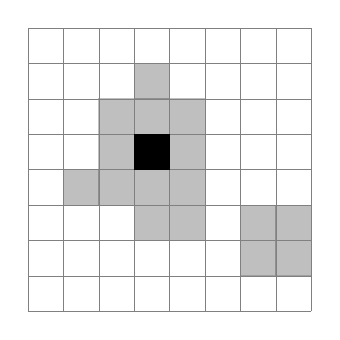
\begin{tikzpicture}[scale=0.45]
			\draw[help lines, step=1] (-4, -4) grid (4, 4);
			\foreach \x in {(-3, -1), (-2, -1), (-2, 0), (-2, 1), (-1, -2), (-1, -1), (-1, 0), (-1, 1), (-1, 2), (0, -2), (0, -1), (0, 0), (0, 1), (2, -3), (2, -2), (3, -3), (3, -2)}
				\filldraw[gray, opacity=0.5] \x rectangle + (1, 1);
			\foreach \x in {(-1, 0)}
				\filldraw[black] \x rectangle + (1, 1);
		\end{tikzpicture}
		\caption{Result of binary erosion of \ref{fig: openingbefore} with a $3 \times 3$ pixel structuring element. The light gray pixels are set to zero.}
		\label{fig: openingerosion}
	\end{subfigure}
	\vfill
	\begin{subfigure}[t]{0.45\linewidth}
		\centering
		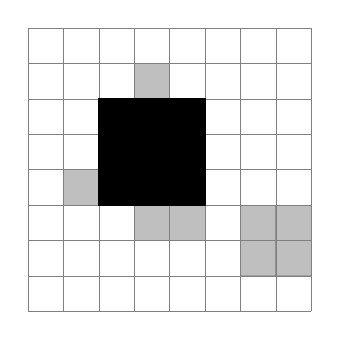
\begin{tikzpicture}[scale=0.45]
			\draw[help lines, step=1] (-4, -4) grid (4, 4);
			\foreach \x in {(-3, -1), (-1, -2), (-1, 2), (0, -2), (2, -3), (2, -2), (3, -3), (3, -2)}
				\filldraw[gray, opacity=0.5] \x rectangle + (1, 1);
			\foreach \x in {(-2, -1), (-2, 0), (-2, 1), (-1, -1), (-1, 0), (-1, 1), (0, -1), (0, 0), (0, 1)}
				\filldraw[black] \x rectangle + (1, 1);
		\end{tikzpicture}
		\caption{Binary dilation of the black pixel in \ref{fig: openingerosion} with a $3 \times 3$ pixel structuring element. The original image is displayed as light gray.}
		\label{fig: openingdilation}
	\end{subfigure}
	\hfill
	\begin{subfigure}[t]{0.45\linewidth}
		\centering
		
\begin{tikzpicture}[scale=0.45]
			\draw[help lines, step=1] (-4, -4) grid (4, 4);
			\foreach \x in {(-2, -1), (-2, 0), (-2, 1), (-1, -1), (-1, 0), (-1, 1), (0, -1), (0, 0), (0, 1)}
				\filldraw[black] \x rectangle + (1, 1);
		\end{tikzpicture}
		\caption{Result of opening of \ref{fig: openingbefore} with a $3 \times 3$ pixel structuring element. Outliers have been eliminated and edges have been smoothed.}
		\label{fig: openingafter}
	\end{subfigure}
	\caption{Example of binary morphological opening using a $3 \times 3$ pixel structuring element.}
	\label{fig: exampleopening}
\end{figure}

Edges of the larger connected region have been smoothed, making morphological opening a great tool for the smoothing of edges and outlier elimination \cite[p.~69]{imageprocessing}.\\

Figure \ref{fig: exampleclosing} shows an example of binary morphological closing with a $3 \times 3$ pixel structuring element.

% Draw example of morphological closing:
\begin{figure}[ht]
	\centering
	\begin{subfigure}[t]{0.45\linewidth}
		\centering
		
\begin{tikzpicture}[scale=0.45]
			\draw[help lines, step=1] (-4, -4) grid (4, 4);
			\foreach \x in {(-2, 0), (-2, 2), (1, 1), (1, -2)}
				\filldraw[black] \x rectangle + (1, 1);
		\end{tikzpicture}
		\caption{Binary image.}
		\label{fig: closingbefore}
	\end{subfigure}
	\hfill
	\begin{subfigure}[t]{0.45\linewidth}
		\centering
		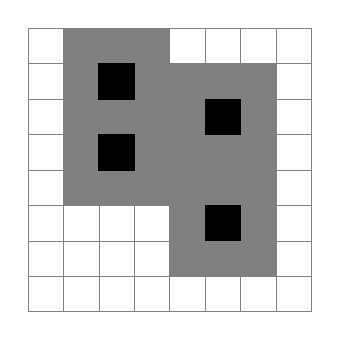
\begin{tikzpicture}[scale=0.45]
			\draw[help lines, step=1] (-4, -4) grid (4, 4);
			\foreach \x in {(-3, -1), (-3, 0), (-3, 1), (-3, 2), (-3, 3), (-2, -1), (-2, 0), (-2, 1), (-2, 2), (-2, 3), (-1, -1), (-1, 0), (-1, 1), (-1, 2), (-1, 3), (0, -3), (0, -2), (0, -1), (0, 0), (0, 1), (0, 2), (1, -3), (1, -2), (1, -1), (1, 0), (1, 1), (1, 2), (2, -3), (2, -2), (2, -1), (2, 0), (2, 1), (2, 2)}
				\filldraw[gray] \x rectangle + (1, 1);
			\foreach \x in {(-2, 0), (-2, 2), (1, 1), (1, -2)}
				\filldraw[black] \x rectangle + (1, 1);
		\end{tikzpicture}
		\caption{Image after binary dilation with a $3 \times 3$ pixel structuring element. The dark gray pixels are now set to one.}
		\label{fig: closingdilation}
	\end{subfigure}
	\vfill
	\begin{subfigure}[t]{0.45\linewidth}
		\centering
		
\begin{tikzpicture}[scale=0.45]
			\draw[help lines, step=1] (-4, -4) grid (4, 4);
			\foreach \x in {(-3, -1), (-3, 0), (-3, 1), (-3, 2), (-3, 3), (-2, -1), (-2, 3), (-1, -1), (-1, 2), (-1, 3), (0, -3), (0, -2), (0, -1), (0, 2), (1, -3), (1, 2), (2, -3), (2, -2), (2, -1), (2, 0), (2, 1), (2, 2)}
				\filldraw[gray, opacity=0.5] \x rectangle + (1, 1);
			\foreach \x in {(-2, 0), (-2, 1), (-2, 2), (-1, 0), (-1, 1), (0, 0), (0, 1), (1, -2), (1, -1), (1, 0), (1, 1)}
				\filldraw[gray] \x rectangle + (1, 1);
			\foreach \x in {(-2, 0), (-2, 2), (1, 1), (1, -2)}
				\filldraw[black] \x rectangle + (1, 1);
		\end{tikzpicture}
		\caption{Image after binary closing, i.e. dilation and erosion. The light gray pixels are set to zero again.}
		\label{fig: closingerosion}
	\end{subfigure}
	\hfill
	\begin{subfigure}[t]{0.45\linewidth}
		\centering
		
\begin{tikzpicture}[scale=0.45]
			\draw[help lines, step=1] (-4, -4) grid (4, 4);
			\foreach \x in {(-2, 0), (-2, 1), (-2, 2), (-1, 0), (-1, 1), (0, 0), (0, 1), (1, -2), (1, -1), (1, 0), (1, 1)}
				\filldraw[black] \x rectangle + (1, 1);
		\end{tikzpicture}
		\caption{Result of closing. The gaps between pixels have been filled.}
		\label{fig: closingafter}
	\end{subfigure}
	\caption{Example of binary morphological closing.}
	\label{fig: exampleclosing}
\end{figure}

Morphological closing is frequently used as a tool to fill gaps in binary images, see Fig. \ref{fig: exampleclosing} and \cite[p.~69]{imageprocessing}.

Altogether, both morphological opening and closing are effective tools to smooth edges. Morphological opening achieves this by eliminating outliers, while morphological closing fills gaps.

\newpage



\section{Main results}\label{section: mainresults}

In the following, we consider the effect of morphological opening and closing on the upper bounds for the error probabilities in the statistical test developed in Section \ref{section: statisticalmodel}. Note, that under morphological opening and closing we have $\Theta \circ \Psi \subseteq \Theta \subseteq \Theta \bullet \Psi$ for any structuring element $\Psi$. From this fact we deduce, that morphological opening will lower the probabiliy of a type I error, but increase the probability of a type II error. Morphological closing, on the other hand, has the opposite effect. While this serves as a qualitative argument for the employment of these operators, we aim at quantifying this change of the probabilities by proving upper bounds for the error probabilities after morphological opening and closing have been applied.

We use a square structuring element, since we have the prior information, that the region of interest in the image is rectangular.

The changes of the upper bound for the probability of a type I error after opening and after opening and closing with a square structuring element are quantified in the following theorem.

\begin{theorem}\label{thm: typeIinequalities}
	Let $m, n \in \mathbb{N}$, $c \in \mathbb{R} \setminus \{ 0 \}$ and $\Omega = \left\{ 1, \dots, m \right\} \times \left\{ 1, \dots, n \right\}$. Assume that $F$ follows the statistical model given in \eqref{statmodel2}.
	
	For a statistical significance $\alpha \in (0, 1)$, let $t_\alpha$ be a threshold, such that $\mathbb{P}_V( \norm{\Delta^+ F(\tilde{i}, \tilde{j})} \geq t_\alpha ) \leq \alpha$ for every $(\tilde{i}, \tilde{j}) \in \Omega$ and $V \in \mathcal{H}_0^+(\tilde{i}, \tilde{j})$ and $\mathbb{P}_V( \norm{\Delta^- F(\tilde{i}, \tilde{j})} \geq t_\alpha ) \leq \alpha$ for every $(\tilde{i}, \tilde{j}) \in \Omega$ and $V \in \mathcal{H}_0^-(\tilde{i}, \tilde{j})$, cf. \eqref{setH0+} and \eqref{setH0-}.
	
	Let $\mathfrak{I}_\alpha$ be the binary image defined by
	\begin{equation*}
		\mathfrak{I}_\alpha(\tilde{i}, \tilde{j}) = \mathds{1}_{ \{ T(\tilde{i}, \tilde{j}) \geq t_\alpha \} }
	\end{equation*}
	for all $(\tilde{i}, \tilde{j}) \in \Omega$.
	
	Let $(i, j) \in \Omega$ and let $T(i, j)$ be the test statistic defined in \eqref{teststatistic} and $H_0(i, j)$ be the null hypothesis defined in \eqref{nullhypothesis}.
	
	Let $\varphi \in \mathbb{N}$ be odd and define the set $\Phi_\varphi = \left\{ -\frac{\varphi - 1}{2}, -\frac{\varphi - 3}{2}, \dots, \frac{\varphi - 3}{2}, \frac{\varphi - 1}{2} \right\}$ and the structuring element $\Psi_\varphi = \Phi_\varphi \times \Phi_\varphi$.
	Then for $V \in \mathcal{H}_0(i, j)$ the following inequalities hold:
	\begin{align}
		\mathbb{P}_V\left( (\mathfrak{I}_\alpha \circ \Psi_\varphi)(i, j) = 1 \right) &\leq \varphi \alpha^{\frac{\varphi + 1}{2}} \label{ineq: typeIopening} \\
		\mathbb{P}_V\left( ((\mathfrak{I}_\alpha \circ \Psi_\varphi) \bullet \Psi_\varphi)(i, j) = 1 \right) &\leq \varphi^3 \alpha^{\frac{\varphi + 1}{2}} \label{ineq: typeIclosing}
	\end{align}
\end{theorem}
\begin{proof}
	We start with the proof of inequality \eqref{ineq: typeIopening}. We aim to find an upper bound for the probability
	\begin{equation*}
		\mathbb{P}_V\left( (\mathfrak{I}_\alpha \circ \Psi_\varphi)(i, j) = 1 \right)
	\end{equation*}
	for $V \in \mathcal{H}_0(i, j)$.
	
	As discussed in Section \ref{section: definitions}, any matrix $V \in \mathcal{V}_c^{m, n}$ is uniquely defined by the top left corner $(\kappa_1, \lambda_1)$ and bottom right corner $(\kappa_2, \lambda_2)$ of the rROI $\varLambda = \{ \kappa_1, \dots, \kappa_2 \} \times \{ \lambda_1, \dots, \lambda_2 \}$ contained in $V$, where $\varLambda$ is defined as in Definition \ref{def: rROIcheckerboard}.
	
	Since $V \in \mathcal{H}_0(i, j)$ we have $(i, j) \notin \varLambda$ implying, that $i < \kappa_1$ or $j < \lambda_1$ or $i > \kappa_2$ or $j > \lambda_2$. These four cases are not mutually exclusive. As deducted in Section \ref{section: statisticalmodel}, the first two cases imply $\norm{\Delta^- V(i, j)} = 0$ and the latter two imply $\norm{\Delta^+ V(i, j)} = 0$.
	
	Based on this knowledge, we can split up the sets $\mathcal{H}_0^+(i, j)$ and $\mathcal{H}_0^-(i, j)$ as defined in \eqref{setH0+} and \eqref{setH0-} by defining the sets
	\begin{align*}
		\mathcal{H}_0^{(1)}(i, j) &\coloneqq \left\{ V \in \mathcal{V}_c^{m, n} \mid V(\tilde{i}, \tilde{j}) = 0 \textrm{ for all } (\tilde{i}, \tilde{j}) \in \{ 1, \dots, i \} \times \{ 1, \dots, n \} \right\}, \\
		\mathcal{H}_0^{(2)}(i, j) &\coloneqq \left\{ V \in \mathcal{V}_c^{m, n} \mid V(\tilde{i}, \tilde{j}) = 0 \textrm{ for all } (\tilde{i}, \tilde{j}) \in \{ 1, \dots, m \} \times \{ 1, \dots, j \} \right\}, \\
		\mathcal{H}_0^{(3)}(i, j) &\coloneqq \left\{ V \in \mathcal{V}_c^{m, n} \mid V(\tilde{i}, \tilde{j}) = 0 \textrm{ for all } (\tilde{i}, \tilde{j}) \in \{ i, \dots, m \} \times \{ 1, \dots, n \} \right\}, \\
		\mathcal{H}_0^{(4)}(i, j) &\coloneqq \left\{ V \in \mathcal{V}_c^{m, n} \mid V(\tilde{i}, \tilde{j}) = 0 \textrm{ for all } (\tilde{i}, \tilde{j}) \in \{ 1, \dots, m \} \times \{ j, \dots, n \} \right\}.
	\end{align*}
	Note, that $\mathcal{H}_0^-(i, j) = \mathcal{H}_0^{(1)}(i, j) \cup \mathcal{H}_0^{(2)}(i, j)$ and $\mathcal{H}_0^+(i, j) = \mathcal{H}_0^{(3)}(i, j) \cup \mathcal{H}_0^{(4)}(i, j)$. Furthermore, this implies $\mathcal{H}_0(i, j) = \bigcup_{u = 1}^4 \mathcal{H}_0^{(u)}(i, j)$.
	
	Assume the first case, i.e. $V \in \mathcal{H}_0^{(1)}(i, j)$. It follows, that
	\begin{equation*}
		\norm{\Delta^- V(i, 1)} = \ldots = \norm{\Delta^- V(i, n)} = 0.
	\end{equation*}
	implying $V \in \bigcap_{\tilde{j} = 1}^n \mathcal{H}_0^-(i, \tilde{j})$.
	
	In a first step, we use equation \eqref{eq: openingset} and the fact, that $\Psi_\varphi = \Phi_\varphi \times \Phi_\varphi$ to write the left hand side of inequality \eqref{ineq: typeIopening} as
	\begin{align*}
		\mathbb{P}_V&\left( (\mathfrak{I}_\alpha \circ \Psi_\varphi)(i, j) = 1 \right) \\
		&= \mathbb{P}_V\left( \bigcup_{(k, \ell) \in \Psi_\varphi} \bigcap_{(\tilde{k}, \tilde{\ell}) \in \Psi_\varphi} \left\{ \mathfrak{I}_\alpha(i - k + \tilde{k}, j - \ell + \tilde{\ell}) = 1 \right\} \right) \\
		&= \mathbb{P}_V\left( \bigcup_{k, \ell \in \Phi_\varphi} \bigcap_{\tilde{k}, \tilde{\ell} \in \Phi_\varphi} \left\{ \mathfrak{I}_\alpha(i - k + \tilde{k}, j - \ell + \tilde{\ell}) = 1 \right\} \right).
	\end{align*}
	
	Using sub-additivity we can bound this from above by writing it as a sum over $\ell \in \Phi_\varphi$ to get
	\begin{align*}
		\mathbb{P}_V&\left( (\mathfrak{I}_\alpha \circ \Psi_\varphi)(i, j) = 1 \right) \\
		&\leq \sum_{\ell \in \Phi_\varphi} \mathbb{P}_V\left( \bigcup_{k \in \Phi_\varphi} \bigcap_{\tilde{k}, \tilde{\ell} \in \Phi_\varphi} \left\{ \mathfrak{I}_\alpha(i - k + \tilde{k}, j - \ell + \tilde{\ell}) = 1 \right\} \right).
	\end{align*}
	
	By dropping every term except for $\tilde{k} = k$ in the inner intersection, we obtain
	\begin{align*}
		\mathbb{P}_V&\left( (\mathfrak{I}_\alpha \circ \Psi_\varphi)(i, j) = 1 \right) \\
		&\leq \sum_{\ell \in \Phi_\varphi} \mathbb{P}_V\left( \bigcup_{k \in \Phi_\varphi} \bigcap_{\tilde{k} = k, \tilde{\ell} \in \Phi_\varphi} \left\{ \mathfrak{I}_\alpha(i - k + \tilde{k}, j - \ell + \tilde{\ell}) = 1 \right\} \right) \\
		&= \sum_{\ell \in \Phi_\varphi} \mathbb{P}_V\left( \bigcup_{k \in \Phi_\varphi} \bigcap_{\tilde{\ell} \in \Phi_\varphi} \left\{ \mathfrak{I}_\alpha(i, j - \ell + \tilde{\ell}) = 1 \right\} \right).
	\end{align*}
	
	The events inside the probability do not depend on $k \in \Phi_\varphi$ anymore, which yields
	\begin{equation*}
		\bigcup_{k \in \Phi_\varphi} \bigcap_{\tilde{\ell} \in \Phi_\varphi} \left\{ \mathfrak{I}_\alpha(i, j - \ell + \tilde{\ell}) = 1 \right\} = \bigcap_{\tilde{\ell} \in \Phi_\varphi} \left\{ \mathfrak{I}_\alpha(i, j - \ell + \tilde{\ell}) = 1 \right\}.
	\end{equation*}
	
	Plugging this in, we obtain
	\begin{equation*}
		\mathbb{P}_V\left( (\mathfrak{I}_\alpha \circ \Psi_\varphi)(i, j) = 1 \right) \leq \sum_{\ell \in \Phi_\varphi} \mathbb{P}_V\left( \bigcap_{\tilde{\ell} \in \Phi_\varphi} \left\{ \mathfrak{I}_\alpha(i, j - \ell + \tilde{\ell}) = 1 \right\} \right).
	\end{equation*}
	
	We have defined the binary $\mathfrak{I}_\alpha$ by setting $\mathfrak{I}_\alpha(\tilde{i}, \tilde{j}) = \mathds{1}_{ \{ T(\tilde{i}, \tilde{j}) \geq t_\alpha \} }$. Using this definition and the definition of $T(i, j)$ we can rewrite the upper bound as
	\begin{align*}
		&\sum_{\ell \in \Phi_\varphi} \mathbb{P}_V\left( \bigcap_{\tilde{\ell} \in \Phi_\varphi} \left\{ \mathfrak{I}_\alpha(i, j - \ell + \tilde{\ell}) = 1 \right\} \right) \\
		&= \sum_{\ell \in \Phi_\varphi} \mathbb{P}_V\left( \bigcap_{\tilde{\ell} \in \Phi_\varphi} \left\{ T(i, j - \ell + \tilde{\ell}) \geq t_\alpha \right\} \right) \\
		&= \sum_{\ell \in \Phi_\varphi} \mathbb{P}_V\left( \bigcap_{\tilde{\ell} \in \Phi_\varphi} \left( \left\{ \norm{\Delta^+ F(i, j - \ell + \tilde{\ell})} \geq t_\alpha \right\} \cap \left\{ \norm{\Delta^- F(i, j - \ell + \tilde{\ell})} \geq t_\alpha \right\} \right) \right).
	\end{align*}
	
	In the case $V \in \mathcal{H}_0^{(1)}(i, j) \subseteq \mathcal{H}_0^-(i, j)$, the values of $\norm{\Delta^+ V(i, j - \ell + \tilde{\ell})}$ are unknown. Thus, we do not know the distribution of the random variables $\norm{\Delta^+ F(i, j - \ell + \tilde{\ell})}$ and we drop the events $\left\{ \norm{\Delta^+ F(i, j - \ell + \tilde{\ell})} \geq t_\alpha \right\}$ to obtain
	\begin{align*}
		\mathbb{P}_V&\left( (\mathfrak{I}_\alpha \circ \Psi_\varphi)(i, j) = 1 \right) \\
		&\leq \sum_{\ell \in \Phi_\varphi} \mathbb{P}_V\left( \bigcap_{\tilde{\ell} \in \Phi_\varphi} \left( \left\{ \norm{\Delta^+ F(i, j - \ell + \tilde{\ell})} \geq t_\alpha \right\} \cap \left\{ \norm{\Delta^- F(i, j - \ell + \tilde{\ell})} \geq t_\alpha \right\} \right) \right) \\
		&\leq \sum_{\ell \in \Phi_\varphi} \mathbb{P}_V\left( \bigcap_{\tilde{\ell} \in \Phi_\varphi} \left\{ \norm{\Delta^- F(i, j - \ell + \tilde{\ell})} \geq t_\alpha \right\} \right).
	\end{align*}
	
	Define a subset $\tilde{\Phi}_\varphi = \left\{ -\frac{\varphi - 1}{2}, -\frac{\varphi - 5}{2}, \dots, \frac{\varphi - 5}{2}, \frac{\varphi - 1}{2} \right\}$ of $\Phi_\varphi$. Since $\Delta^- F(i, j)$ only depends on the pixels $(i, j), (i - 1, j)$ and $(i, j - 1)$, the set $\left\{ \norm{\Delta^- F(i, j - \ell + \tilde{\ell})} \mid \tilde{\ell} \in \tilde{\Phi}_\varphi \right\}$ is a set of independent random variables for fixed $\ell \in \Phi_\varphi$, see Figure \ref{fig: independentpoints}.
	
	% Draw picture of independent pixels:
	\begin{figure}[h]
	\centering
	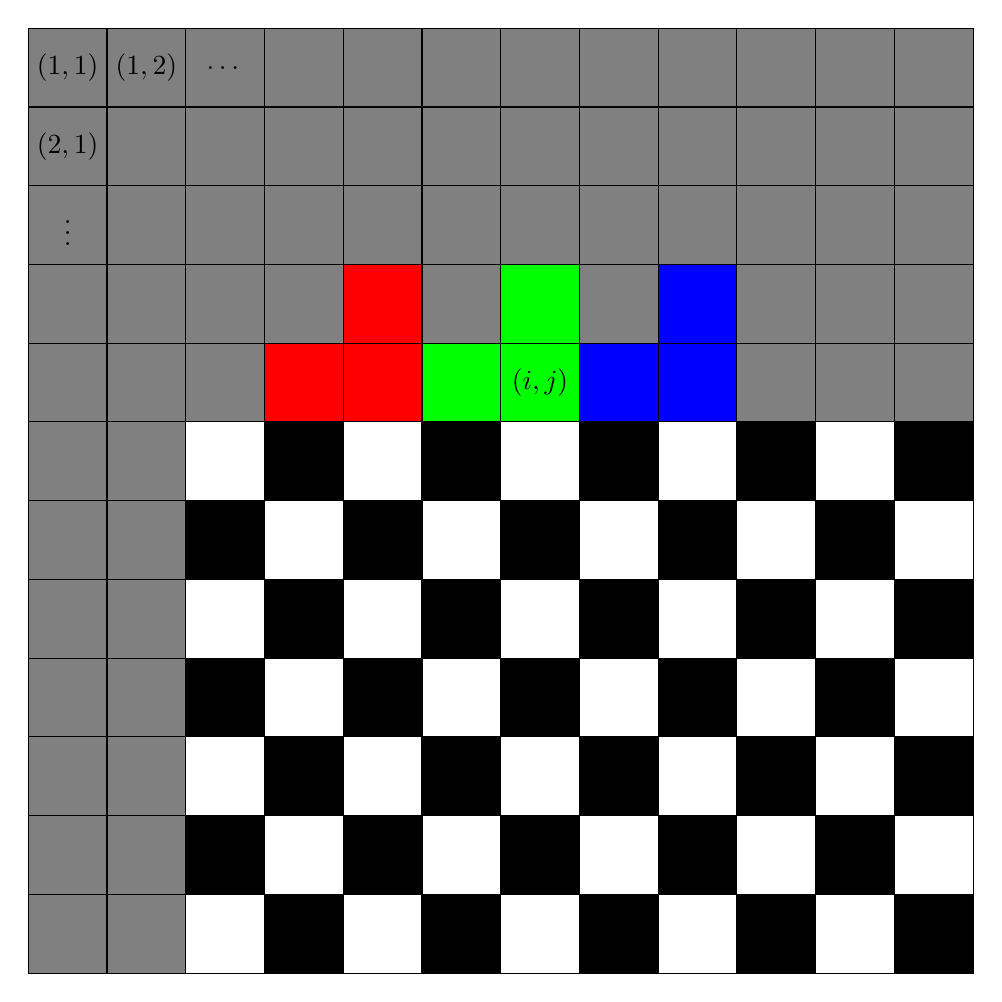
\begin{tikzpicture}
		\foreach \i in {-6, ..., 5}
			\foreach \j in {-6, ..., 5}
				\filldraw[gray] (\i, \j) rectangle + (1, 1);
		\foreach \i in {-4, ..., 5}
			\foreach \j in {-6, ..., 0}
				{
					\pgfmathparse{mod(\i+\j, 2) ? "black" : "white"}
					\edef\colour{\pgfmathresult}
					\filldraw[fill=\colour] (\i, \j) rectangle + (1, 1);
				}
		\foreach \x in {(-2, 1), (-3, 1), (-2, 2)}
			\filldraw[red] \x rectangle + (1, 1);
		\foreach \x in {(0, 1), (-1, 1), (0, 2)}
			\filldraw[green] \x rectangle + (1, 1);
		\foreach \x in {(2, 1), (1, 1), (2, 2)}
			\filldraw[blue] \x rectangle + (1, 1);
		\draw[step=1] (-6, -6) grid (6, 6);
		\node at (0.5, 1.5) {$(i, j)$};
		\node at (-5.5, 5.5) {$(1, 1)$};
		\node at (-4.5, 5.5) {$(1, 2)$};
		\node at (-3.5, 5.5) {$\dots$};
		\node at (-5.5, 4.5) {$(2, 1)$};
		\node at (-5.5, 3.5) {$\vdots$};
	\end{tikzpicture}
	\caption{The random variable $\norm{\Delta^- F(i, j)}$ only depends on the green pixels, $\norm{\Delta^- F(i, j - 2)}$ depends on the red pixels and $\norm{\Delta^- F(i, j + 2)}$ on the blue pixels. Since these are all distinct from another, the random variables are independent.}
	\label{fig: independentpoints}
\end{figure}
	
	We drop the terms in $\Phi_\varphi \setminus \tilde{\Phi}_\varphi$ and use the independence to obtain
	\begin{align*}
		\mathbb{P}_V\left( (\mathfrak{I}_\alpha \circ \Psi_\varphi)(i, j) = 1 \right) &\leq \sum_{\ell \in \Phi_\varphi} \mathbb{P}_V\left( \bigcap_{\tilde{\ell} \in \Phi_\varphi} \left\{ \norm{\Delta^- F(i, j - \ell + \tilde{\ell})} \geq t_\alpha \right\} \right) \\
		&\leq \sum_{\ell \in \Phi_\varphi} \mathbb{P}_V\left( \bigcap_{\tilde{\ell} \in \tilde{\Phi}_\varphi} \left\{ \norm{\Delta^- F(i, j - \ell + \tilde{\ell})} \geq t_\alpha \right\} \right) \\
		&= \sum_{\ell \in \Phi_\varphi} \prod_{\tilde{\ell} \in \tilde{\Phi}_\varphi} \mathbb{P}_V\left( \norm{\Delta^- F(i, j - \ell + \tilde{\ell})} \geq t_\alpha \right).
	\end{align*}
	
	Since $V \in \mathcal{H}_0^{(1)}(i, j)$, we have
	\begin{equation*}
		V \in \bigcap_{\tilde{j} = 1}^n \mathcal{H}_0^-(i, \tilde{j}) \subseteq \bigcap_{\ell \in \Phi_\varphi, \tilde{\ell} \in \tilde{\Phi}_\varphi} \mathcal{H}_0^-(i, j - \ell + \tilde{\ell}).
	\end{equation*}
	
	By assumption, $\mathbb{P}_V\left( \norm{\Delta^- F(i, j)} \geq t_\alpha \right) \leq \alpha$ for $V \in \mathcal{H}_0^-(i, j)$ yielding the upper bound
	\begin{align*}
		\mathbb{P}_V\left( (\mathfrak{I}_\alpha \circ \Psi_\varphi)(i, j) = 1 \right) &\leq \sum_{\ell \in \Phi_\varphi} \prod_{\tilde{\ell} \in \tilde{\Phi}_\varphi} \mathbb{P}_V\left( \norm{\Delta^- F(i, j - \ell + \tilde{\ell})} \geq t_\alpha \right) \\
		&\leq \sum_{\ell \in \Phi_\varphi} \prod_{\tilde{\ell} \in \tilde{\Phi}_\varphi} \alpha \\
		&= \abs{\Phi_\varphi} \alpha^{\abs{\tilde{\Phi}_\varphi}} \\
		&= \varphi \alpha^{\frac{\varphi + 1}{2}}.
	\end{align*}
	
	This proves the first inequality for $V \in \mathcal{H}_0^{(1)}(i, j)$. The other three cases can be proven analogously by swapping the roles of $k$ or $\tilde{k}$ with $\ell$ or $\tilde{\ell}$, respectively and/or by replacing $\Delta^-$ by $\Delta^+$. This finishes the proof of the first inequality.\\
	
	
	For the proof of the second inequality, we exploit our prior knowledge on $V$ again. As already stated in the proof of the first inequality, we have, that $H_0(i, j)$ is equivalent to $(i, j) \notin \varLambda$, which is equivalent to at least one of the cases $V \in \mathcal{H}_0^{(u)}(i, j)$ for $u \in \{ 1, 2, 3, 4 \}$.
	
	Again, we assume the first case, i.e. $V \in \mathcal{H}_0^{(1)}(i, j)$. This implies, that the null hypotheses $H_0(\tilde{i}, 1), \ldots, H_0(\tilde{i}, n)$ are true for all $\tilde{i} \in \{ 1, \dots, i \}$. It also implies
	\begin{equation*}
		\norm{\Delta^- V(\tilde{i}, 1)} = \ldots = \norm{\Delta^- V(\tilde{i}, n)} = 0
	\end{equation*}
	for all $\tilde{i} \in \{ 1, \dots, i \}$.
	
	Set $k_0 = -\frac{\varphi - 1}{2}$ and $\ell_0 = 0$. Then $(k_0, \ell_0) \in \Psi_\varphi$ and we get that the null hypotheses $H_0(i + k_0 - \tilde{k}, j + \ell_0 - \tilde{\ell})$ are true for all $\tilde{k}, \tilde{\ell} \in \Phi_\varphi$. Hence, we have $V \in \bigcap_{\tilde{k}, \tilde{\ell} \in \Phi_\varphi} \mathcal{H}_0(i + k_0 - \tilde{k}, j - \tilde{\ell})$ as well as $\norm{\Delta^- V(i + k_0 - \tilde{k}, j + \ell_0 - \tilde{\ell})} = 0$ for all $\tilde{k}, \tilde{\ell} \in \Phi_\varphi$.
	
	Define $\mathfrak{K}_\alpha = \mathfrak{I}_\alpha \circ \Psi_\varphi$. We use equation \eqref{eq: closingset} and $\Psi_\varphi = \Phi_\varphi \times \Phi_\varphi$ to write the left hand side of inequality \eqref{ineq: typeIclosing} as
	\begin{align*}
		\mathbb{P}_V&\left( (\mathfrak{K}_\alpha \bullet \Psi_\varphi)(i, j) = 1 \right) \\
		&= \mathbb{P}_V\left( \bigcap_{(k, \ell) \in \Psi_\varphi} \bigcup_{(\tilde{k}, \tilde{\ell}) \in \Psi_\varphi} \left\{ \mathfrak{K}_\alpha(i + k - \tilde{k}, j + \ell - \tilde{\ell}) = 1 \right\} \right) \\
		&= \mathbb{P}_V\left( \bigcap_{k, \ell \in \Phi_\varphi} \bigcup_{\tilde{k}, \tilde{\ell} \in \Phi_\varphi} \left\{ \mathfrak{K}_\alpha(i + k - \tilde{k}, j + \ell - \tilde{\ell}) = 1 \right\} \right).
	\end{align*}
	
	By dropping every term in the intersection except for $k = k_0$ and $\ell = \ell_0$ we can bound this from above by
	\begin{align*}
		\mathbb{P}_V\left( (\mathfrak{K}_\alpha \bullet \Psi_\varphi)(i, j) = 1 \right) &= \mathbb{P}_V\left( \bigcap_{k, \ell \in \Phi_\varphi} \bigcup_{\tilde{k}, \tilde{\ell} \in \Phi_\varphi} \left\{ \mathfrak{K}_\alpha(i + k - \tilde{k}, j + \ell - \tilde{\ell}) = 1 \right\} \right) \\
		&\leq \mathbb{P}_V\left( \bigcup_{\tilde{k}, \tilde{\ell} \in \Phi_\varphi} \left\{ \mathfrak{K}_\alpha(i + k_0 - \tilde{k}, j + \ell_0 - \tilde{\ell}) = 1 \right\} \right) \\
		&= \mathbb{P}_V\left( \bigcup_{\tilde{k}, \tilde{\ell} \in \Phi_\varphi} \left\{ \mathfrak{K}_\alpha(i + k_0 - \tilde{k}, j - \tilde{\ell}) = 1 \right\} \right).
	\end{align*}
	
	Using sub-additivity to write this as the sum over all $\tilde{k}, \tilde{\ell} \in \Phi_\varphi$ yields
	\begin{equation*}
		\mathbb{P}_V\left( (\mathfrak{K}_\alpha \bullet \Psi_\varphi)(i, j) = 1 \right) \leq \sum_{\tilde{k}, \tilde{\ell} \in \Phi_\varphi} \mathbb{P}_V\left( \mathfrak{K}_\alpha(i + k_0 - \tilde{k}, j - \tilde{\ell}) = 1 \right).
	\end{equation*}
	
	Plugging in the definition of $\mathfrak{K}_\alpha$ we obtain
	\begin{equation*}
		\mathbb{P}_V\left( (\mathfrak{K}_\alpha \bullet \Psi_\varphi)(i, j) = 1 \right) \leq \sum_{\tilde{k}, \tilde{\ell} \in \Phi_\varphi} \mathbb{P}_V\left( (\mathfrak{I}_\alpha \circ \Psi_\varphi)(i + k_0 - \tilde{k}, j - \tilde{\ell}) = 1 \right).
	\end{equation*}
	
	As discussed, we have $V \in \bigcap_{\tilde{k}, \tilde{\ell} \in \Phi_\varphi} \mathcal{H}_0(i + k_0 - \tilde{k}, j - \tilde{\ell})$. Thus, we can use inequality \eqref{ineq: typeIopening} to get the upper bound
	\begin{align*}
		\mathbb{P}_V\left( (\mathfrak{K}_\alpha \bullet \Psi_\varphi)(i, j) = 1 \right) &\leq \sum_{\tilde{k}, \tilde{\ell} \in \Phi_\varphi} \mathbb{P}_V\left( (\mathfrak{I}_\alpha \circ \Psi_\varphi)(i + k_0 - \tilde{k}, j - \tilde{\ell}) = 1 \right) \\
		&\leq \sum_{\tilde{k}, \tilde{\ell} \in \Phi_\varphi} \varphi \alpha^{\frac{\varphi + 1}{2}} \\
		&= \varphi^3 \alpha^{\frac{\varphi + 1}{2}}.
	\end{align*}
	
	This proves the inequality for $V \in \mathcal{H}_0^{(1)}(i, j)$. The other cases are proven analogously by taking $k_0 = 0, \ell_0 = -\frac{\varphi - 1}{2}$ in the second case, $k_0 = \frac{\varphi - 1}{2}, \ell_0 = 0$ in the third case and $k_0 = 0, \ell_0 = \frac{\varphi - 1}{2}$ in the fourth case. In the second and fourth case, the roles of $\Delta^+$ and $\Delta^-$ are swapped. This finishes the proof of the second inequality and thus the proof of the theorem.
\end{proof}

\begin{remark}
	The bounds in Theorem \ref{thm: typeIinequalities} hold for all background pixels. This means, they also hold for the worst case, i.e. pixels, that lie adjacent to the region of interest, see Figure \ref{fig: independentpoints}.
\end{remark}

\begin{remark}
	We require the threshold $t_\alpha$ in Theorem \ref{thm: typeIinequalities} to satisfy stronger conditions than $\mathbb{P}_V( T(i, j) \geq t_\alpha ) \leq \alpha$ for every $V \in \mathcal{H}_0(i, j)$. Since the methods developed in Section \ref{section: boundtypeIerror} yield thresholds, that meet these stronger requirements, we use them to achieve better bounds in Theorem \ref{thm: typeIinequalities}.
\end{remark}

Let us consider the probability of a type II error in the statistical test. In Section \ref{section: analyzetypeIIerror} we numerically calculated bounds for this probability. Similar to the previous theorem, we aim at quantifying the change of the upper bound after morphological opening and closing are applied.

We will need the additional assumption, that the region of interest is sufficiently large, i.e. larger than the structuring element. Otherwise, even if there are no errors in the binarization through the statistical test, morphological opening will classify all pixels as background and thus the probability of a type II error cannot be bounded anymore.

\begin{theorem}\label{thm: typeIIinequalities}
	Let $m, n \in \mathbb{N}$, $c \in \mathbb{R} \setminus \{ 0 \}$ and $\Omega = \left\{ 1, \dots, m \right\} \times \left\{ 1, \dots, n \right\}$. Assume that $F$ follows the statistical model given in \eqref{statmodel2}.
	
	Let $t$ be a threshold, such that
	\begin{equation*}
		\mathbb{P}_V\left( T(\tilde{i}, \tilde{j}) \leq t \right) \leq \beta
	\end{equation*}
	for some $\beta \in (0, 1)$ and all $(\tilde{i}, \tilde{j}) \in \Omega$ and $V \in \mathcal{H}_1(\tilde{i}, \tilde{j})$, cf. \eqref{setH1}.
	
	Let $\mathfrak{I}$ be the binary image defined by
	\begin{equation*}
		\mathfrak{I}(\tilde{i}, \tilde{j}) = \mathds{1}_{ \{ T(\tilde{i}, \tilde{j}) \geq t \} }
	\end{equation*}
	for all $(\tilde{i}, \tilde{j}) \in \Omega$.
	
	Let $(i, j) \in \Omega$ and let $T(i, j)$ be the test statistic defined in \eqref{teststatistic} and $H_1(i, j)$ be the alternative hypothesis defined in \eqref{alternativehypothesis}.
	
	Let $\varphi \in \mathbb{N}$ be odd and define the set $\Phi_\varphi = \left\{ -\frac{\varphi - 1}{2}, -\frac{\varphi - 3}{2}, \dots, \frac{\varphi - 3}{2}, \frac{\varphi - 1}{2} \right\}$ and the structuring element $\Psi_\varphi = \Phi_\varphi \times \Phi_\varphi$.
	
	Denote by $\varLambda = \{ \kappa_1, \dots, \kappa_2 \} \times \{ \lambda_1, \dots, \lambda_2 \}$ the rROI contained in $V$. Let $\min \{ \kappa_2 - \kappa_1 + 1, \lambda_2 - \lambda_1 + 1 \} \geq \varphi$.
	Then for $V \in \mathcal{H}_1(i, j)$ the following inequalities hold:
	\begin{align}
		\mathbb{P}_V\left( (\mathfrak{I} \circ \Psi_\varphi)(i, j) = 0 \right) &\leq \varphi^2 \beta \label{ineq: typeIIopening} \\
		\mathbb{P}_V\left( ((\mathfrak{I} \circ \Psi_\varphi) \bullet \Psi_\varphi)(i, j) = 0 \right) &\leq \varphi^2 \beta \label{ineq: typeIIclosing}
	\end{align}
\end{theorem}
\begin{proof}
	We start by proving inequality \eqref{ineq: typeIIopening}. We use a similar approach as in Theorem \ref{thm: typeIinequalities} by finding indices $(k_0, \ell_0) \in \Psi_\varphi$, such that the alternative hypotheses $H_1(i - k_0 + \tilde{k}, j - \ell_0 + \tilde{\ell})$ are true for all $\tilde{k}, \tilde{\ell} \in \Phi_\varphi$. Figure \ref{fig: setofforegroundpixels} shows, that we can find such indices even for the case of a corner pixel. A constructive proof can be found in Appendix \ref{appendix: proofs}.
	
	% Draw picture of foreground pixels:
	\begin{figure}[h]
	\centering
	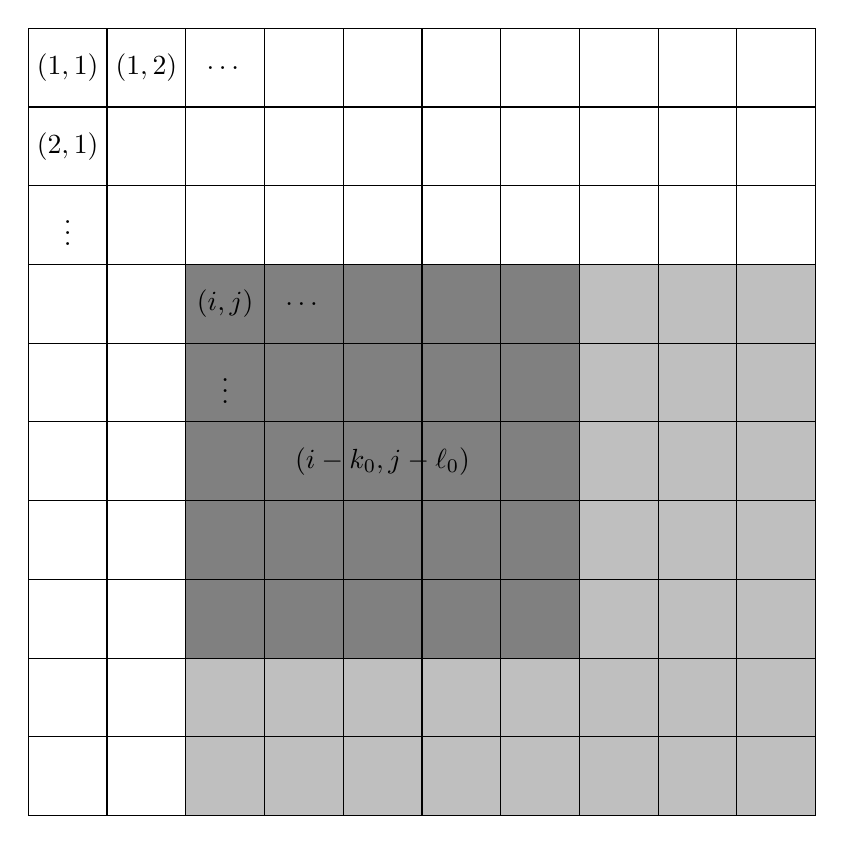
\begin{tikzpicture}
		\foreach \i in {-5, ..., 4}
			\foreach \j in {-5, ..., 4}
				\filldraw[white] (\i, \j) rectangle + (1, 1);
		\foreach \i in {-3, ..., 4}
			\foreach \j in {-5, ..., 1}
				\filldraw[gray, opacity=0.5] (\i, \j) rectangle + (1, 1);
		\foreach \i in {-3, ..., 1}
			\foreach \j in {-3, ..., 1}
				\filldraw[gray] (\i, \j) rectangle + (1, 1);
		\draw[step=1] (-5, -5) grid (5, 5);
		\node at (-2.5, 1.5) {$(i, j)$};
		\node at (-1.5, 1.5) {$\dots$};
		\node at (-2.5, 0.5) {$\vdots$};
		\node at (-0.5, -0.5) {$(i - k_0, j - \ell_0)$};
		\node at (-4.5, 4.5) {$(1, 1)$};
		\node at (-3.5, 4.5) {$(1, 2)$};
		\node at (-2.5, 4.5) {$\dots$};
		\node at (-4.5, 3.5) {$(2, 1)$};
		\node at (-4.5, 2.5) {$\vdots$};
	\end{tikzpicture}
	\caption{White pixels represent background, light gray pixels represent foreground. The indices $(k_0, \ell_0) \in \Psi_\varphi$ are chosen, such that for all $\tilde{k}, \tilde{\ell} \in \Phi_\varphi$ the pixels $(i - k_0 + \tilde{k}, j - \ell_0 + \tilde{\ell})$ belong to the foreground. These pixels are marked as dark gray.}
	\label{fig: setofforegroundpixels}
\end{figure}
	
	The alternative hypotheses $H_1(i - k_0 + \tilde{k}, j - \ell_0 + \tilde{\ell})$ being true for all $\tilde{k}, \tilde{\ell} \in \Phi_\varphi$ implies $V \in \bigcap_{\tilde{k}, \tilde{\ell} \in \Phi_\varphi} \mathcal{H}_1(i - k_0 + \tilde{k}, j - \ell_0 + \tilde{\ell})$.
	
	We start by using equation \eqref{eq: openingset} and $\Psi_\varphi = \Phi_\varphi \times \Phi_\varphi$ to write the left hand side of inequality \eqref{ineq: typeIIopening} as
	\begin{align*}
		\mathbb{P}_V\left( (\mathfrak{I} \circ \Psi_\varphi)(i, j) = 0 \right) &= \mathbb{P}_V\left( \bigcap_{(k, \ell) \in \Psi_\varphi} \bigcup_{(\tilde{k}, \tilde{\ell}) \in \Psi_\varphi} \left\{ \mathfrak{I}(i - k + \tilde{k}, j - \ell + \tilde{\ell}) = 0 \right\} \right) \\
		&= \mathbb{P}_V\left( \bigcap_{k, \ell \in \Phi_\varphi} \bigcup_{\tilde{k}, \tilde{\ell} \in \Phi_\varphi} \left\{ \mathfrak{I}(i - k + \tilde{k}, j - \ell + \tilde{\ell}) = 0 \right\} \right).
	\end{align*}
	
	We drop every term in the intersection except $k = k_0, \ell = \ell_0$ to bound this by
	\begin{align*}
		\mathbb{P}_V\left( (\mathfrak{I} \circ \Psi_\varphi)(i, j) = 0 \right) &= \mathbb{P}_V\left( \bigcap_{k, \ell \in \Phi_\varphi} \bigcup_{\tilde{k}, \tilde{\ell} \in \Phi_\varphi} \left\{ \mathfrak{I}(i - k + \tilde{k}, j - \ell + \tilde{\ell}) = 0 \right\} \right) \\
		&\leq \mathbb{P}_V\left( \bigcup_{\tilde{k}, \tilde{\ell} \in \Phi_\varphi} \left\{ \mathfrak{I}(i - k_0 + \tilde{k}, j - \ell_0 + \tilde{\ell}) = 0 \right\} \right).
	\end{align*}
	
	We use sub-additivity to write this as the sum over all $\tilde{k}, \tilde{\ell} \in \Phi_\varphi$ and obtain
	\begin{equation*}
		\mathbb{P}_V\left( (\mathfrak{I} \circ \Psi_\varphi)(i, j) = 0 \right) \leq \sum_{\tilde{k}, \tilde{\ell} \in \Phi_\varphi} \mathbb{P}_V\left( \mathfrak{I}(i - k_0 + \tilde{k}, j - \ell_0 + \tilde{\ell}) = 0 \right).
	\end{equation*}
	
	Using the fact, that $V \in \bigcap_{\tilde{k}, \tilde{\ell} \in \Phi_\varphi} \mathcal{H}_1(i - k_0 + \tilde{k}, j - \ell_0 + \tilde{\ell})$ as well as the definition of $\mathfrak{I}$ and the choice of the threshold $t$ we get the upper bound
	\begin{align*}
		\mathbb{P}_V\left( (\mathfrak{I} \circ \Psi_\varphi)(i, j) = 0 \right) &\leq \sum_{\tilde{k}, \tilde{\ell} \in \Phi_\varphi} \mathbb{P}_V\left( \mathfrak{I}(i - k_0 + \tilde{k}, j - \ell_0 + \tilde{\ell}) = 0 \right) \\
		&= \sum_{\tilde{k}, \tilde{\ell} \in \Phi_\varphi} \mathbb{P}_V\left( T(i - k_0 + \tilde{k}, j - \ell_0 + \tilde{\ell}) \leq t \right) \\
		&\leq \sum_{\tilde{k}, \tilde{\ell} \in \Phi_\varphi} \beta \\
		&= \abs{\Phi_\varphi}^2 \beta \\
		&= \varphi^2 \beta.
	\end{align*}
	
	This finishes the proof of the first inequality.\\
	
	
	For the proof of the second inequality, define $\mathfrak{K} = \mathfrak{I} \circ \Psi_\varphi$. By the properties of morphological closing we have $(\mathfrak{K} \bullet \Psi_\varphi)(i, j) \geq \mathfrak{K}(i, j)$ yielding
	\begin{equation*}
		\mathbb{P}_V\left( (\mathfrak{K} \bullet \Psi_\varphi)(i, j) = 0 \right) \leq \mathbb{P}_V\left( \mathfrak{K}(i, j) = 0 \right) = \mathbb{P}_V\left( (\mathfrak{I} \circ \Psi_\varphi)(i, j) = 0 \right).
	\end{equation*}
	
	Since $V \in \mathcal{H}_1(i, j)$, we can apply inequality \eqref{ineq: typeIIopening} and obtain the upper bound
	\begin{align*}
		\mathbb{P}_V\left( (\mathfrak{K} \bullet \Psi_\varphi)(i, j) = 0 \right) &\leq \mathbb{P}_V\left( (\mathfrak{I} \circ \Psi_\varphi)(i, j) = 0 \right) \\
		&\leq \varphi^2 \beta.
	\end{align*}
	
	This proves the second inequality and thus finishes the proof.
\end{proof}

\begin{remark}
	The bounds in the previous theorem hold for all pixels within the region of interest, i.e. also for the edges and corners of the region of interest.
	
	For pixels with a sufficient distance from the edges of the region of interest, we can also prove the upper bound
	\begin{equation*}
		\mathbb{P}_V\left( ((\mathfrak{I} \circ \Psi_\varphi) \bullet \Psi_\varphi)(i, j) = 0 \right) \leq \varphi^{10} \beta^4.
	\end{equation*}
	
	A proof can be found in Appendix \ref{appendix: proofs}. This only improves the bound for very small values of $\beta$.
\end{remark}

We employ morphological closing to reduce the number of type II errors. This is not represented in the upper bound in inequality \eqref{ineq: typeIIclosing}. The simulation results displayed in Section \ref{section: simulationresults} and Appendix \ref{appendix: simulations} show, that the amount of type II errors after opening and after opening and closing behave similarly, when the standard deviation of the noise increases. A small improvement through closing can only be observed for a certain range of standard deviations.

This behaviour is due to the pixels not being independent anymore, after morphological opening has been applied. In some cases, the amount of type II errors is greatly increased through opening and the application of closing only reverts this to a very small extent, cf. Appendix \ref{appendix: simulations} Figure \ref{fig: normal_alpha0.01_phi99}.

Based on these observations, an improvement of the upper bound in inequality \eqref{ineq: typeIIclosing} without improving the upper bound in \eqref{ineq: typeIIopening} seems unlikely.
Note, that any improvements of the upper bound in inequality \eqref{ineq: typeIIopening} can immediately be applied to the upper bound in inequality \eqref{ineq: typeIIclosing} as well.

\newpage



\section{Simulation results}\label{section: simulationresults}

To simulate the error rates of the statistical test and the subsequent application of morphological opening and closing, we create six different types of images, depending on the position of the pixel $(i, j)$ with respect to the region of interest, see Figure \ref{fig: simulatedpixeltypes}.

\begin{figure}[H]
	\centering
	\begin{subfigure}[t]{0.45\linewidth}
		\centering
		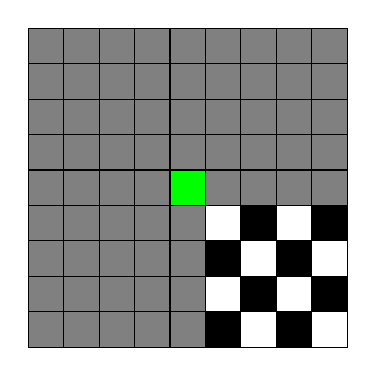
\begin{tikzpicture}[scale=0.45]
			\foreach \i in {-4, ..., 4}
				\foreach \j in {-4, ..., 4}
					\filldraw[gray] (\i, \j) rectangle + (1, 1);
			\foreach \i in {1, ..., 4}
				\foreach \j in {-4, ..., -1}
				{
					\pgfmathparse{mod(\i+\j, 2) ? "black" : "white"}
					\edef\colour{\pgfmathresult}
					\filldraw[fill=\colour] (\i, \j) rectangle + (1, 1);
				}
			\filldraw[green] (0, 0) rectangle + (1, 1);
			\draw[step=1] (-4, -4) grid (5, 5);
		\end{tikzpicture}
		\caption{Background pixel at the corner of the ROI.}
		\label{fig: background_corner}
	\end{subfigure}
	\hfill
	\begin{subfigure}[t]{0.45\linewidth}
		\centering
		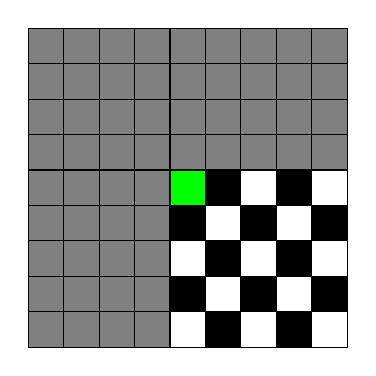
\begin{tikzpicture}[scale=0.45]
			\foreach \i in {-4, ..., 4}
				\foreach \j in {-4, ..., 4}
					\filldraw[gray] (\i, \j) rectangle + (1, 1);
			\foreach \i in {0, ..., 4}
				\foreach \j in {-4, ..., 0}
				{
					\pgfmathparse{mod(\i+\j, 2) ? "black" : "white"}
					\edef\colour{\pgfmathresult}
					\filldraw[fill=\colour] (\i, \j) rectangle + (1, 1);
				}
			\filldraw[green] (0, 0) rectangle + (1, 1);
			\draw[step=1] (-4, -4) grid (5, 5);
		\end{tikzpicture}
		\caption{Foreground pixel at the corner of the ROI.}
		\label{fig: foreground_corner}
	\end{subfigure}
	\vfill
	\begin{subfigure}[t]{0.45\linewidth}
		\centering
		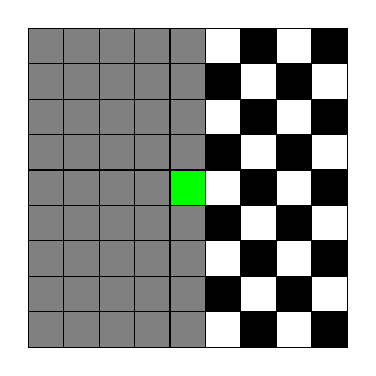
\begin{tikzpicture}[scale=0.45]
			\foreach \i in {-4, ..., 4}
				\foreach \j in {-4, ..., 4}
					\filldraw[gray] (\i, \j) rectangle + (1, 1);
			\foreach \i in {1, ..., 4}
				\foreach \j in {-4, ..., 4}
				{
					\pgfmathparse{mod(\i+\j+1, 2) ? "black" : "white"}
					\edef\colour{\pgfmathresult}
					\filldraw[fill=\colour] (\i, \j) rectangle + (1, 1);
				}
			\filldraw[green] (0, 0) rectangle + (1, 1);
			\draw[step=1] (-4, -4) grid (5, 5);
		\end{tikzpicture}
		\caption{Background pixel at the edge of the ROI.}
		\label{fig: background_edge}
	\end{subfigure}
	\hfill
	\begin{subfigure}[t]{0.45\linewidth}
		\centering
		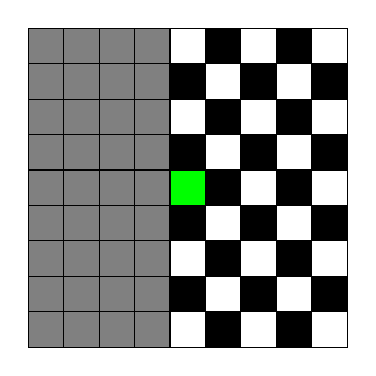
\begin{tikzpicture}[scale=0.45]
			\foreach \i in {-4, ..., 4}
				\foreach \j in {-4, ..., 4}
					\filldraw[gray] (\i, \j) rectangle + (1, 1);
			\foreach \i in {0, ..., 4}
				\foreach \j in {-4, ..., 4}
				{
					\pgfmathparse{mod(\i+\j, 2) ? "black" : "white"}
					\edef\colour{\pgfmathresult}
					\filldraw[fill=\colour] (\i, \j) rectangle + (1, 1);
				}
			\filldraw[green] (0, 0) rectangle + (1, 1);
			\draw[step=1] (-4, -4) grid (5, 5);
		\end{tikzpicture}
		\caption{Foreground pixel at the edge of the ROI.}
		\label{fig: foreground_edge}
	\end{subfigure}
	\vfill
	\begin{subfigure}[t]{0.45\linewidth}
		\centering
		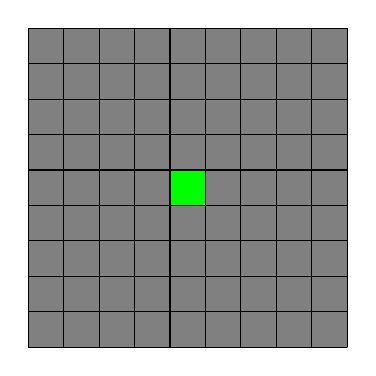
\begin{tikzpicture}[scale=0.45]
			\foreach \i in {-4, ..., 4}
				\foreach \j in {-4, ..., 4}
					\filldraw[gray] (\i, \j) rectangle + (1, 1);
			\filldraw[green] (0, 0) rectangle + (1, 1);
			\draw[step=1] (-4, -4) grid (5, 5);
		\end{tikzpicture}
		\caption{Background pixel surrounded by background.}
		\label{fig: background_free}
	\end{subfigure}
	\hfill
	\begin{subfigure}[t]{0.45\linewidth}
		\centering
		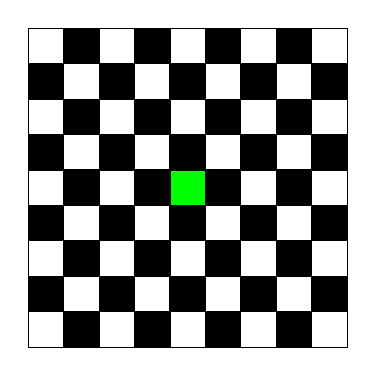
\begin{tikzpicture}[scale=0.45]
			\foreach \i in {-4, ..., 4}
				\foreach \j in {-4, ..., 4}
				{
					\pgfmathparse{mod(\i+\j, 2) ? "black" : "white"}
					\edef\colour{\pgfmathresult}
					\filldraw[fill=\colour] (\i, \j) rectangle + (1, 1);
				}
			\filldraw[green] (0, 0) rectangle + (1, 1);
			\draw[step=1] (-4, -4) grid (5, 5);
		\end{tikzpicture}
		\caption{Foreground pixel surrounded by foreground.}
		\label{fig: foreground_free}
	\end{subfigure}
	\caption{Position of the simulated pixels with respect to the ROI.}
	\label{fig: simulatedpixeltypes}
\end{figure}

The six different types include the best and worst case for identification of a background and foreground pixel, respectively. For both background and foreground pixels to be identified correctly, it is ideal, if the pixel is only surrounded by other background or foreground pixels, see Figures \ref{fig: background_free} and \ref{fig: foreground_free}.
For a background pixel to be correctly identified, the worst case is, if the pixel is located at the edge of the region of interest, see Figure \ref{fig: background_edge}. Similarly, the worst case for a foreground pixel to be correctly identified is to be located at the corner of the region of interest, see Figure \ref{fig: foreground_corner}. While other positions of the pixel $(i, j)$ with respect to the region of interest are possible, our simulations cover the extreme cases. We expect the error rates for other cases to lie between those of the extreme cases.

The images are created by contructing the image and region of interest around the pixel $(i, j)$ according to the target position of the pixel. For each type of image, we randomly generate 1000 noises and add it to the image with standard deviations $\sigma$ ranging from 1 to 150. After binarization through the statistical test, morphological opening and closing, we determine the error rate by dividing the the number of times the pixel is falsely identified by the total number of noises.

In Figure \ref{fig: normal_alpha0.05_phi5} the error rates for $\alpha = 0.05$ and $\varphi = 5$ are displayed. For all simulated positions of background pixels, we keep the error rate after binarization through the statistical test below the target statistical significance through the choice of the threshold. As expected, the error rate is equal to the statistical significance in the worst case for low standard deviations, see Figure \ref{fig: normal_alpha0.05_phi5_background_edge}. Through application of morphological opening and closing, the error rates drop to zero for all standard deviations and all simulated positions of background pixels. For the simulated positions of foreground pixels, the error rates after binarization are zero for small standard deviations and increase, as the standard deviation increases. The better the position of the foreground pixel, the longer the error rate stays close to zero. While the application of morphological opening barely has an impact for small standard deviations, it greatly increases the error rate for higher standard deviations. The subsequent application of morphological closing only decreases the error rate to a very small extent, if at all, making it almost negligible.

\begin{figure}[H]
	\centering
	\begin{subfigure}[t]{0.48\linewidth}
		\centering
		\begin{tikzpicture}
			\begin{axis}[
				legend pos=north west,
				legend style={nodes={scale=0.5, transform shape}},
				xlabel=Standard deviation $\sigma$,
				ylabel=Type I error rate,
				grid=both,
				minor grid style={gray!25},
				major grid style={gray!25},
				ymin=-0.05,
				ymax=1.05,
				width=\linewidth,
				no marks]
				\addplot[line width=1pt,dashed,color=blue] table[x=sigma,y=typeI,col sep=comma]{CSV/CSV_SinglePixel/normal/alpha0.05/phi5/background_corner.csv};
				\addlegendentry{Binarization}
				\addplot[line width=1pt,dashed,color=red] table[x=sigma,y=typeI_o,col sep=comma]{CSV/CSV_SinglePixel/normal/alpha0.05/phi5/background_corner.csv};
				\addlegendentry{Opening}
				\addplot[line width=1pt,dashed,color=gray] table[x=sigma,y=typeI_oc,col sep=comma]{CSV/CSV_SinglePixel/normal/alpha0.05/phi5/background_corner.csv};
				\addlegendentry{Opening \& Closing}
			\end{axis}
		\end{tikzpicture}
		\caption{Background pixel at the corner of the rROI.}
		\label{fig: normal_alpha0.05_phi5_background_corner}
	\end{subfigure}
	\hfill
	\begin{subfigure}[t]{0.48\linewidth}
		\centering
		\begin{tikzpicture}
			\begin{axis}[
				legend pos=north west,
				legend style={nodes={scale=0.5, transform shape}},
				xlabel=Standard deviation $\sigma$,
				ylabel=Type II error rate,
				grid=both,
				minor grid style={gray!25},
				major grid style={gray!25},
				ymin=-0.05,
				ymax=1.05,
				width=\linewidth,
				no marks]
				\addplot[line width=1pt,dashed,color=blue] table[x=sigma,y=typeII,col sep=comma]{CSV/CSV_SinglePixel/normal/alpha0.05/phi5/foreground_corner.csv};
				\addlegendentry{Binarization}
				\addplot[line width=1pt,dashed,color=red] table[x=sigma,y=typeII_o,col sep=comma]{CSV/CSV_SinglePixel/normal/alpha0.05/phi5/foreground_corner.csv};
				\addlegendentry{Opening}
				\addplot[line width=1pt,dashed,color=gray] table[x=sigma,y=typeII_oc,col sep=comma]{CSV/CSV_SinglePixel/normal/alpha0.05/phi5/foreground_corner.csv};
				\addlegendentry{Opening \& Closing}
			\end{axis}
		\end{tikzpicture}
		\caption{Foreground pixel at the corner of the rROI.}
		\label{fig: normal_alpha0.05_phi5_foreground_corner}
	\end{subfigure}
	\vfill
	\begin{subfigure}[t]{0.48\linewidth}
		\centering
		\begin{tikzpicture}
			\begin{axis}[
				legend pos=north west,
				legend style={nodes={scale=0.5, transform shape}},
				xlabel=Standard deviation $\sigma$,
				ylabel=Type I error rate,
				grid=both,
				minor grid style={gray!25},
				major grid style={gray!25},
				ymin=-0.05,
				ymax=1.05,
				width=\linewidth,
				no marks]
				\addplot[line width=1pt,dashed,color=blue] table[x=sigma,y=typeI,col sep=comma]{CSV/CSV_SinglePixel/normal/alpha0.05/phi5/background_edge.csv};
				\addlegendentry{Binarization}
				\addplot[line width=1pt,dashed,color=red] table[x=sigma,y=typeI_o,col sep=comma]{CSV/CSV_SinglePixel/normal/alpha0.05/phi5/background_edge.csv};
				\addlegendentry{Opening}
				\addplot[line width=1pt,dashed,color=gray] table[x=sigma,y=typeI_oc,col sep=comma]{CSV/CSV_SinglePixel/normal/alpha0.05/phi5/background_edge.csv};
				\addlegendentry{Opening \& Closing}
			\end{axis}
		\end{tikzpicture}
		\caption{Background pixel at the edge of the rROI.}
		\label{fig: normal_alpha0.05_phi5_background_edge}
	\end{subfigure}
	\hfill
	\begin{subfigure}[t]{0.48\linewidth}
		\centering
		\begin{tikzpicture}
			\begin{axis}[
				legend pos=north west,
				legend style={nodes={scale=0.5, transform shape}},
				xlabel=Standard deviation $\sigma$,
				ylabel=Type II error rate,
				grid=both,
				minor grid style={gray!25},
				major grid style={gray!25},
				ymin=-0.05,
				ymax=1.05,
				width=\linewidth,
				no marks]
				\addplot[line width=1pt,dashed,color=blue] table[x=sigma,y=typeII,col sep=comma]{CSV/CSV_SinglePixel/normal/alpha0.05/phi5/foreground_edge.csv};
				\addlegendentry{Binarization}
				\addplot[line width=1pt,dashed,color=red] table[x=sigma,y=typeII_o,col sep=comma]{CSV/CSV_SinglePixel/normal/alpha0.05/phi5/foreground_edge.csv};
				\addlegendentry{Opening}
				\addplot[line width=1pt,dashed,color=gray] table[x=sigma,y=typeII_oc,col sep=comma]{CSV/CSV_SinglePixel/normal/alpha0.05/phi5/foreground_edge.csv};
				\addlegendentry{Opening \& Closing}
			\end{axis}
		\end{tikzpicture}
		\caption{Foreground pixel at the edge of the rROI.}
		\label{fig: normal_alpha0.05_phi5_foreground_edge}
	\end{subfigure}
	\vfill
	\begin{subfigure}[t]{0.48\linewidth}
		\centering
		\begin{tikzpicture}
			\begin{axis}[
				legend pos=north west,
				legend style={nodes={scale=0.5, transform shape}},
				xlabel=Standard deviation $\sigma$,
				ylabel=Type I error rate,
				grid=both,
				minor grid style={gray!25},
				major grid style={gray!25},
				ymin=-0.05,
				ymax=1.05,
				width=\linewidth,
				no marks]
				\addplot[line width=1pt,dashed,color=blue] table[x=sigma,y=typeI,col sep=comma]{CSV/CSV_SinglePixel/normal/alpha0.05/phi5/background_free.csv};
				\addlegendentry{Binarization}
				\addplot[line width=1pt,dashed,color=red] table[x=sigma,y=typeI_o,col sep=comma]{CSV/CSV_SinglePixel/normal/alpha0.05/phi5/background_free.csv};
				\addlegendentry{Opening}
				\addplot[line width=1pt,dashed,color=gray] table[x=sigma,y=typeI_oc,col sep=comma]{CSV/CSV_SinglePixel/normal/alpha0.05/phi5/background_free.csv};
				\addlegendentry{Opening \& Closing}
			\end{axis}
		\end{tikzpicture}
		\caption{Background pixel surrounded by background.}
		\label{fig: normal_alpha0.05_phi5_background_free}
	\end{subfigure}
	\hfill
	\begin{subfigure}[t]{0.48\linewidth}
		\centering
		\begin{tikzpicture}
			\begin{axis}[
				legend pos=north west,
				legend style={nodes={scale=0.5, transform shape}},
				xlabel=Standard deviation $\sigma$,
				ylabel=Type II error rate,
				grid=both,
				minor grid style={gray!25},
				major grid style={gray!25},
				ymin=-0.05,
				ymax=1.05,
				width=\linewidth,
				no marks]
				\addplot[line width=1pt,dashed,color=blue] table[x=sigma,y=typeII,col sep=comma]{CSV/CSV_SinglePixel/normal/alpha0.05/phi5/foreground_free.csv};
				\addlegendentry{Binarization}
				\addplot[line width=1pt,dashed,color=red] table[x=sigma,y=typeII_o,col sep=comma]{CSV/CSV_SinglePixel/normal/alpha0.05/phi5/foreground_free.csv};
				\addlegendentry{Opening}
				\addplot[line width=1pt,dashed,color=gray] table[x=sigma,y=typeII_oc,col sep=comma]{CSV/CSV_SinglePixel/normal/alpha0.05/phi5/foreground_free.csv};
				\addlegendentry{Opening \& Closing}
			\end{axis}
		\end{tikzpicture}
		\caption{Foreground pixel surrounded by foreground.}
		\label{fig: normal_alpha0.05_phi5_foreground_free}
	\end{subfigure}
	\caption{Error rates after binarization, opening and closing. The $x$-axes display the standard deviation $\sigma$ and the $y$-axes the error rate. For each pixel type 1000 different noises were randomly generated $(\alpha = 0.05, \varphi = 5)$.}
	\label{fig: normal_alpha0.05_phi5}
\end{figure}

This observation can be explained as follows. As the standard deviation increases, type II errors become more numerous. Thus, there are more falsely identified pixels within the region of interest after binarization. Morphological opening connects these falsely identified pixels, also misclassifying the pixels between the initial falsely classified pixels. This can create clusters the size of the structuring element of falsely identified pixels within the region of interest. Morphological closing with the same structuring element cannot fix these errors.

Theorem \ref{thm: typeIinequalities} yields another approach to the extraction of the region of interest. Using a relaxed statistical significance $\tilde{\alpha} = \left( \frac{\alpha}{\varphi^3} \right)^{\frac{2}{\varphi + 1}}$ to calculate the threshold $t_{\tilde{\alpha}}$, yields
\begin{equation*}
	\mathbb{P}_V\left( ((\mathfrak{I}_{\tilde{\alpha}} \circ \Psi_\varphi) \bullet \Psi_\varphi)(i, j) = 1 \right) \leq \varphi^3 \left( \left( \frac{\alpha}{\varphi^3} \right)^{\frac{2}{\varphi + 1}} \right)^{\frac{\varphi + 1}{2}} \leq \alpha
\end{equation*}
by inequality \eqref{ineq: typeIclosing}. This way, we can bound the probability of a type I error after opening and closing below a given statistical significance $\alpha$. The error rates for this approach with $\alpha = 0.05$ and $\varphi = 5$ are displayed in Figure \ref{fig: relaxed_alpha0.05_phi5}. The error rates for background pixels after opening and closing are below the given statistical significance $\alpha$, while the errors rates for foreground pixels are slightly lower than in Figure \ref{fig: normal_alpha0.05_phi5}.

Simulations for other structuring elements as well as for $\alpha = 0.01$ can be found in Appendix \ref{appendix: simulations}. The code used for the simulation can be found in Appendix \ref{appendix: algorithms}.

\begin{figure}[H]
	\centering
	\begin{subfigure}[t]{0.48\linewidth}
		\centering
		\begin{tikzpicture}
			\begin{axis}[
				legend pos=north west,
				legend style={nodes={scale=0.5, transform shape}},
				xlabel=Standard deviation $\sigma$,
				ylabel=Type I error rate,
				grid=both,
				minor grid style={gray!25},
				major grid style={gray!25},
				ymin=-0.05,
				ymax=1.05,
				width=\linewidth,
				no marks]
				\addplot[line width=1pt,dashed,color=blue] table[x=sigma,y=typeI,col sep=comma]{CSV/CSV_SinglePixel/relaxed/alpha0.05/phi5/background_corner.csv};
				\addlegendentry{Binarization}
				\addplot[line width=1pt,dashed,color=red] table[x=sigma,y=typeI_o,col sep=comma]{CSV/CSV_SinglePixel/relaxed/alpha0.05/phi5/background_corner.csv};
				\addlegendentry{Opening}
				\addplot[line width=1pt,dashed,color=gray] table[x=sigma,y=typeI_oc,col sep=comma]{CSV/CSV_SinglePixel/relaxed/alpha0.05/phi5/background_corner.csv};
				\addlegendentry{Opening \& Closing}
			\end{axis}
		\end{tikzpicture}
		\caption{Background pixel at the corner of the rROI.}
		\label{fig: relaxed_alpha0.05_phi5_background_corner}
	\end{subfigure}
	\hfill
	\begin{subfigure}[t]{0.48\linewidth}
		\centering
		\begin{tikzpicture}
			\begin{axis}[
				legend pos=north west,
				legend style={nodes={scale=0.5, transform shape}},
				xlabel=Standard deviation $\sigma$,
				ylabel=Type II error rate,
				grid=both,
				minor grid style={gray!25},
				major grid style={gray!25},
				ymin=-0.05,
				ymax=1.05,
				width=\linewidth,
				no marks]
				\addplot[line width=1pt,dashed,color=blue] table[x=sigma,y=typeII,col sep=comma]{CSV/CSV_SinglePixel/relaxed/alpha0.05/phi5/foreground_corner.csv};
				\addlegendentry{Binarization}
				\addplot[line width=1pt,dashed,color=red] table[x=sigma,y=typeII_o,col sep=comma]{CSV/CSV_SinglePixel/relaxed/alpha0.05/phi5/foreground_corner.csv};
				\addlegendentry{Opening}
				\addplot[line width=1pt,dashed,color=gray] table[x=sigma,y=typeII_oc,col sep=comma]{CSV/CSV_SinglePixel/relaxed/alpha0.05/phi5/foreground_corner.csv};
				\addlegendentry{Opening \& Closing}
			\end{axis}
		\end{tikzpicture}
		\caption{Foreground pixel at the corner of the rROI.}
		\label{fig: relaxed_alpha0.05_phi5_foreground_corner}
	\end{subfigure}
	\vfill
	\begin{subfigure}[t]{0.48\linewidth}
		\centering
		\begin{tikzpicture}
			\begin{axis}[
				legend pos=north west,
				legend style={nodes={scale=0.5, transform shape}},
				xlabel=Standard deviation $\sigma$,
				ylabel=Type I error rate,
				grid=both,
				minor grid style={gray!25},
				major grid style={gray!25},
				ymin=-0.05,
				ymax=1.05,
				width=\linewidth,
				no marks]
				\addplot[line width=1pt,dashed,color=blue] table[x=sigma,y=typeI,col sep=comma]{CSV/CSV_SinglePixel/relaxed/alpha0.05/phi5/background_edge.csv};
				\addlegendentry{Binarization}
				\addplot[line width=1pt,dashed,color=red] table[x=sigma,y=typeI_o,col sep=comma]{CSV/CSV_SinglePixel/relaxed/alpha0.05/phi5/background_edge.csv};
				\addlegendentry{Opening}
				\addplot[line width=1pt,dashed,color=gray] table[x=sigma,y=typeI_oc,col sep=comma]{CSV/CSV_SinglePixel/relaxed/alpha0.05/phi5/background_edge.csv};
				\addlegendentry{Opening \& Closing}
			\end{axis}
		\end{tikzpicture}
		\caption{Background pixel at the edge of the rROI.}
		\label{fig: relaxed_alpha0.05_phi5_background_edge}
	\end{subfigure}
	\hfill
	\begin{subfigure}[t]{0.48\linewidth}
		\centering
		\begin{tikzpicture}
			\begin{axis}[
				legend pos=north west,
				legend style={nodes={scale=0.5, transform shape}},
				xlabel=Standard deviation $\sigma$,
				ylabel=Type II error rate,
				grid=both,
				minor grid style={gray!25},
				major grid style={gray!25},
				ymin=-0.05,
				ymax=1.05,
				width=\linewidth,
				no marks]
				\addplot[line width=1pt,dashed,color=blue] table[x=sigma,y=typeII,col sep=comma]{CSV/CSV_SinglePixel/relaxed/alpha0.05/phi5/foreground_edge.csv};
				\addlegendentry{Binarization}
				\addplot[line width=1pt,dashed,color=red] table[x=sigma,y=typeII_o,col sep=comma]{CSV/CSV_SinglePixel/relaxed/alpha0.05/phi5/foreground_edge.csv};
				\addlegendentry{Opening}
				\addplot[line width=1pt,dashed,color=gray] table[x=sigma,y=typeII_oc,col sep=comma]{CSV/CSV_SinglePixel/relaxed/alpha0.05/phi5/foreground_edge.csv};
				\addlegendentry{Opening \& Closing}
			\end{axis}
		\end{tikzpicture}
		\caption{Foreground pixel at the edge of the rROI.}
		\label{fig: relaxed_alpha0.05_phi5_foreground_edge}
	\end{subfigure}
	\vfill
	\begin{subfigure}[t]{0.48\linewidth}
		\centering
		\begin{tikzpicture}
			\begin{axis}[
				legend pos=north west,
				legend style={nodes={scale=0.5, transform shape}},
				xlabel=Standard deviation $\sigma$,
				ylabel=Type I error rate,
				grid=both,
				minor grid style={gray!25},
				major grid style={gray!25},
				ymin=-0.05,
				ymax=1.05,
				width=\linewidth,
				no marks]
				\addplot[line width=1pt,dashed,color=blue] table[x=sigma,y=typeI,col sep=comma]{CSV/CSV_SinglePixel/relaxed/alpha0.05/phi5/background_free.csv};
				\addlegendentry{Binarization}
				\addplot[line width=1pt,dashed,color=red] table[x=sigma,y=typeI_o,col sep=comma]{CSV/CSV_SinglePixel/relaxed/alpha0.05/phi5/background_free.csv};
				\addlegendentry{Opening}
				\addplot[line width=1pt,dashed,color=gray] table[x=sigma,y=typeI_oc,col sep=comma]{CSV/CSV_SinglePixel/relaxed/alpha0.05/phi5/background_free.csv};
				\addlegendentry{Opening \& Closing}
			\end{axis}
		\end{tikzpicture}
		\caption{Background pixel surrounded by background.}
		\label{fig: relaxed_alpha0.05_phi5_background_free}
	\end{subfigure}
	\hfill
	\begin{subfigure}[t]{0.48\linewidth}
		\centering
		\begin{tikzpicture}
			\begin{axis}[
				legend pos=north west,
				legend style={nodes={scale=0.5, transform shape}},
				xlabel=Standard deviation $\sigma$,
				ylabel=Type II error rate,
				grid=both,
				minor grid style={gray!25},
				major grid style={gray!25},
				ymin=-0.05,
				ymax=1.05,
				width=\linewidth,
				no marks]
				\addplot[line width=1pt,dashed,color=blue] table[x=sigma,y=typeII,col sep=comma]{CSV/CSV_SinglePixel/relaxed/alpha0.05/phi5/foreground_free.csv};
				\addlegendentry{Binarization}
				\addplot[line width=1pt,dashed,color=red] table[x=sigma,y=typeII_o,col sep=comma]{CSV/CSV_SinglePixel/relaxed/alpha0.05/phi5/foreground_free.csv};
				\addlegendentry{Opening}
				\addplot[line width=1pt,dashed,color=gray] table[x=sigma,y=typeII_oc,col sep=comma]{CSV/CSV_SinglePixel/relaxed/alpha0.05/phi5/foreground_free.csv};
				\addlegendentry{Opening \& Closing}
			\end{axis}
		\end{tikzpicture}
		\caption{Foreground pixel surrounded by foreground.}
		\label{fig: relaxed_alpha0.05_phi5_foreground_free}
	\end{subfigure}
	\caption{Error rates after binarization, opening and closing. The $x$-axes display the standard deviation $\sigma$ and the $y$-axes the error rate. For each pixel type 1000 different noises were randomly generated $\left( \tilde{\alpha} = \left( \frac{0.05}{5^3} \right)^{\frac{2}{5 + 1}}, \varphi = 5 \right)$.}
	\label{fig: relaxed_alpha0.05_phi5}
\end{figure}

\newpage



\section{Discussion}\label{section: conclusion}

In this thesis we consider how the upper bounds for the error probabilities of a statistical test change, when morphological opening and closing are applied. To this end, we examine a simplified model and develop a thresholding method to extract the region of interest. The simplified model and thresholding method are designed, such that the probability of a type I error can be bound by a given statistical significance. This is achieved by computing a suitable threshold based on the target statistical significance.

Theorems \ref{thm: typeIinequalities} and \ref{thm: typeIIinequalities} quantify upper bounds for the error rates after morphological opening and closing are applied to the outcome of the statistical test. The upper bounds are stated in terms of the structuring element and the upper bounds for the error probabilities before morphological operations are applied. This was done by exploiting prior knowledge of properties of the region of interest.

In particular, we were able to obtain the exponent $\frac{\varphi + 1}{2}$ in inequality \eqref{ineq: typeIopening} through the choice of the structuring element. For a background pixel to be falsely identified as foreground after opening, at least $\frac{\varphi + 1}{2}$ many pixels background pixels have to be falsely categorized by the binarization through the statistical test. This is the \emph{minimum number of independent points in a structuring element} that can lead to a false categorization of a background pixel.

A different shaped structuring element could lead to no improvements of the error probabilities. To see this, consider a diamond shaped structuring element. A background pixel at the edge of the region of interest, cf. Figure \ref{fig: background_edge}, that is falsely classified by the statistical test, would not be correctly identified as a background pixel, when morphological opening with a diamond shaped structuring element is applied. Thus, the upper bound of this probability in this case does not decrease through application of morphological opening. Hence, we see, that the choice of the structuring element is substantial.

Since we only considered the categorization of a single pixel, a natural next step could be an expansion beyond the scope of this thesis by applying techniques from the field of multiple testing. When researching the connection between multiple testing and morphological operations, one might consider more morphological operators. Namely, the convex hull operator is of high interest in the extraction of the region of interest of a fingerprint.

Generalizations of the results from Sections \ref{section: statisticalmodel} and \ref{section: boundtypeIerror} to convex regions of interest with a checkerboard pattern are possible. For the reasons described above, the choice of the structuring element for a convex region of interest is a question to ponder on. Advances could be achieved in conjunction with multiple testing techniques, since the choice of the structuring element is mainly a limiting factor for pixels close to the edge of the region of interest, which form only a subset of the total pixels in the image.

\newpage



\printbibliography[heading=bibintoc]

\newpage



% Settings for Matlab code inclusion
\definecolor{mygreen}{rgb}{0,0.6,0}
\definecolor{mygray}{rgb}{0.5,0.5,0.5}
\definecolor{mymauve}{rgb}{0.58,0,0.82}
\lstset{ 
	backgroundcolor=\color{white},   % choose the background color; you must add \usepackage{color} or \usepackage{xcolor}; should come as last argument
	basicstyle=\footnotesize,        % the size of the fonts that are used for the code
	breakatwhitespace=false,         % sets if automatic breaks should only happen at whitespace
	breaklines=true,                 % sets automatic line breaking
	captionpos=b,                    % sets the caption-position to bottom
	commentstyle=\color{mygreen},    % comment style
	deletekeywords={...},            % if you want to delete keywords from the given language
	escapeinside={\%*}{*)},          % if you want to add LaTeX within your code
	extendedchars=true,              % lets you use non-ASCII characters; for 8-bits encodings only, does not work with UTF-8
	firstnumber=1,                	 % start line enumeration with line 1
	frame=single,	                 % adds a frame around the code
	keepspaces=true,                 % keeps spaces in text, useful for keeping indentation of code (possibly needs columns=flexible)
	keywordstyle=\color{blue},       % keyword style
	language=Matlab,                 % the language of the code
	morekeywords={*,...},            % if you want to add more keywords to the set
	numbers=left,                    % where to put the line-numbers; possible values are (none, left, right)
	numbersep=5pt,                   % how far the line-numbers are from the code
	numberstyle=\tiny\color{mygray}, % the style that is used for the line-numbers
	rulecolor=\color{black},         % if not set, the frame-color may be changed on line-breaks within not-black text (e.g. comments (green here))
	showspaces=false,                % show spaces everywhere adding particular underscores; it overrides 'showstringspaces'
	showstringspaces=false,          % underline spaces within strings only
	showtabs=false,                  % show tabs within strings adding particular underscores
	stepnumber=1,                    % the step between two line-numbers. If it's 1, each line will be numbered
	stringstyle=\color{mymauve},     % string literal style
	tabsize=2 	                     % sets default tabsize to 2 spaces
}

\begin{appendix}
	\section{Additional proofs}\label{appendix: proofs}
	
%	Define
%	\begin{align*}
%	k_0 &= \min \left\{ i - \kappa_1 - \frac{\varphi - 1}{2}, 0 \right\} - \min \left\{ \kappa_2 - i - \frac{\varphi - 1}{2}, 0 \right\}, \\
%	l_0 &= \min \left\{ j - \lambda_1 - \frac{\varphi - 1}{2}, 0 \right\} - \min \left\{ \lambda_2 - j - \frac{\varphi - 1}{2}, 0 \right\}.
%	\end{align*}
%	
%	First we show, that $k_0$ can only take the values $i - \kappa_1 - \frac{\varphi - 1}{2}$, $- \kappa_2 + i + \frac{\varphi - 1}{2}$ or $0$. Then we distinguish the three possbile cases to show, that $\kappa_1 \leq i - k_0 + \tilde{k} \leq \kappa_2$ in every case. Similarly, we obtain $\lambda_1 \leq j - \ell_0 + \tilde{\ell} \leq \lambda_2$ and hence the alternative hypotheses $H_1(i - k_0 + \tilde{k}, j - \ell_0 + \tilde{\ell})$ are true for all $\tilde{k}, \tilde{\ell} \in \Phi_\varphi$.
%	
%	If $i - \kappa_1 - \frac{\varphi - 1}{2} \leq 0$, by using the assumption $\kappa_2 - \kappa_1 + 1 \geq \varphi$ we obtain
%	\begin{align*}
%	\kappa_2 - i - \frac{\varphi - 1}{2} &= \kappa_2 - i - \frac{\varphi - 1}{2} + \left( i - \kappa_1 - \frac{\varphi - 1}{2} \right) - \left( i - \kappa_1 - \frac{\varphi - 1}{2} \right) \\
%	&= \kappa_2 - \kappa_1 + 1 - \varphi - i + \kappa_1 + \frac{\varphi - 1}{2} \\
%	&\geq - i + \kappa_1 + \frac{\varphi - 1}{2} \\
%	&\geq 0
%	\end{align*}
%	and thus $k_0 = i - \kappa_1 - \frac{\varphi - 1}{2}$. On the other hand, if $\kappa_2 - i - \frac{\varphi - 1}{2} \leq 0$, we obtain
%	\begin{align*}
%	i - \kappa_1 - \frac{\varphi - 1}{2} &= i - \kappa_1 - \frac{\varphi - 1}{2} + \left( \kappa_2 - i - \frac{\varphi - 1}{2} \right) - \left( \kappa_2 - i - \frac{\varphi - 1}{2} \right) \\
%	&= \kappa_2 - \kappa_1 + 1 - \varphi - \kappa_2 + i + \frac{\varphi - 1}{2} \\
%	&\geq - \kappa_2 + i + \frac{\varphi - 1}{2} \\
%	&\geq 0
%	\end{align*}
%	and hence $k_0 = - \kappa_2 + i + \frac{\varphi - 1}{2}$, which shows, that $k_0$ can only take the values $i - \kappa_1 - \frac{\varphi - 1}{2}$, $- \kappa_2 + i + \frac{\varphi - 1}{2}$ or $0$.
%	
%	Assume $k_0 = 0$. This implies $i - \kappa_1 - \frac{\varphi - 1}{2} \geq 0$ as well as $\kappa_2 - i - \frac{\varphi - 1}{2} \geq 0$ and thus for $\tilde{k} \in \Phi_\varphi$ we get
%	\begin{equation*}
%	\kappa_1 \leq i - \frac{\varphi - 1}{2} \leq i + \tilde{k} = i - k_0 + \tilde{k} = i + \tilde{k} \leq i + \frac{\varphi - 1}{2} \leq \kappa_2.
%	\end{equation*}
%	
%	Now assume $k_0 = i - \kappa_1 - \frac{\varphi - 1}{2}$. Then $i - k_0 + \tilde{k} = \kappa_1 + \frac{\varphi - 1}{2} + \tilde{k}$. Using $\kappa_2 - \kappa_1 + 1 \geq \varphi$ yields for every $\tilde{k} \in \Phi_\varphi$
%	\begin{align*}
%	\kappa_1 &= \kappa_1 + \frac{\varphi - 1}{2} - \frac{\varphi - 1}{2} \\
%	&\leq \kappa_1 + \frac{\varphi - 1}{2} + \tilde{k} \\
%	&\leq \kappa_1 + \frac{\varphi - 1}{2} + \frac{\varphi - 1}{2} \\
%	&= \kappa_1 + \varphi - 1 \\
%	&\leq \kappa_2
%	\end{align*}
%	which proves the second case.
%	
%	Lastly, assume $k_0 = - \kappa_2 + i + \frac{\varphi - 1}{2}$. Then $i - k_0 + \tilde{k} = \kappa_2 - \frac{\varphi - 1}{2} + \tilde{k}$. Again, by $\kappa_2 - \kappa_1 + 1 \geq \varphi$ we obtain for every $\tilde{k} \in \Phi_\varphi$
%	\begin{align*}
%	\kappa_1 &\leq \kappa_2 - \varphi + 1 \\
%	&= \kappa_2 - \frac{\varphi - 1}{2} - \frac{\varphi - 1}{2} \\
%	&\leq \kappa_2 - \frac{\varphi - 1}{2} + \tilde{k} \\
%	&\leq \kappa_2 - \frac{\varphi - 1}{2} + \frac{\varphi - 1}{2} \\
%	&= \kappa_2.
%	\end{align*}
	
	\begin{theorem}
		Let $m, n \in \mathbb{N}$, $c \in \mathbb{R} \setminus \{ 0 \}$ and $\Omega = \left\{ 1, \dots, m \right\} \times \left\{ 1, \dots, n \right\}$.
		
		Assume that $F$ follows the statistical model given in \eqref{statmodel2} and let $T(i, j)$ be the test statistic as defined in \eqref{teststatistic} and $H_1(i, j)$ be the alternative hypothesis as defined in \eqref{alternativehypothesis}. Let $t$ be a threshold, such that
		\begin{equation*}
			\mathbb{P}_V\left( T(i, j) \leq t \right) \leq \beta
		\end{equation*}
		for all $V \in \mathcal{H}_1(i, j)$. Let $\mathfrak{I}$ be the binary image defined by
		\begin{equation}
			\mathfrak{I}(i, j) = \mathds{1}_{ \{ T(i, j) \geq t \} }
		\end{equation}
		for all $(i, j) \in \Omega$.
		
		Let $\varphi \in \mathbb{N}$ be odd. Let $\Phi_\varphi = \{ -\frac{\varphi - 1}{2}, -\frac{\varphi - 3}{2}, \dots, \frac{\varphi - 3}{2}, \frac{\varphi - 1}{2} \}$ and $\Psi_\varphi = \Phi_\varphi \times \Phi_\varphi$ be a structuring element.
		
		Denote by $\varLambda = \{ \kappa_1, \dots, \kappa_2 \} \times \{ \lambda_1, \dots, \lambda_2 \}$ the rROI contained in $V$. Let $\min \{ \kappa_2 - \kappa_1 + 1, \lambda_2 - \lambda_1 + 1 \} \geq \varphi$. Let $V \in \mathcal{H}_1(i, j)$ and $(i, j) \in \Omega$ be such, that
		\begin{equation}
			\begin{aligned}
				i - 2 \varphi + 2 &\geq \kappa_1, \\
				i + 2 \varphi - 2 &\leq \kappa_2, \\
				j - 2 \varphi + 2 &\geq \lambda_1, \\
				j + 2 \varphi - 2 &\leq \lambda_2.
			\end{aligned}
		\end{equation}
		Then the following inequalitiy holds:
		\begin{equation}
			\mathbb{P}_V\left( ((\mathfrak{I} \circ \Psi_\varphi) \bullet \Psi_\varphi)(i, j) = 0 \right) \leq \varphi^{10} \beta^4
		\end{equation}
	\end{theorem}
	\begin{proof}
		The assumptions on $(i, j) \in \Omega$ assure, that the alternative hypotheses $H_1(i + k - \tilde{k} - r + \tilde{r}, j + \ell - \tilde{\ell} - s + \tilde{s})$ are true for all $k, \ell, r, s, \tilde{k}, \tilde{\ell}, \tilde{r}, \tilde{s} \in \Phi_\varphi$.
		
		Using equalities \eqref{eq: openingset} and \eqref{eq: closingset} and $\Psi_\varphi = \Phi_\varphi \times \Phi_\varphi$ yields
		\begin{align*}
			\mathbb{P}&_V\left( ((\mathfrak{I} \circ \Psi_\varphi) \bullet \Psi_\varphi)(i, j) = 0 \right) \\
			&= \mathbb{P}_V\left( \bigcup_{(k, \ell) \in \Psi_\varphi} \bigcap_{(\tilde{k}, \tilde{\ell}) \in \Psi_\varphi} \bigcap_{(r, s) \in \Psi_\varphi} \bigcup_{(\tilde{r}, \tilde{s}) \in \Psi_\varphi} \{ \mathfrak{I}(i + k - \tilde{k} - r + \tilde{r}, j + \ell - \tilde{\ell} - s + \tilde{s}) = 0 \} \right) \\
			&= \mathbb{P}_V\left( \bigcup_{k, \ell \in \Phi_\varphi} \bigcap_{\tilde{k}, \tilde{\ell} \in \Phi_\varphi} \bigcap_{r, s \in \Phi_\varphi} \bigcup_{\tilde{r}, \tilde{s} \in \Phi_\varphi} \{ \mathfrak{I}(i + k - \tilde{k} - r + \tilde{r}, j + \ell - \tilde{\ell} - s + \tilde{s}) = 0 \} \right).
		\end{align*}
		
		By sub-additivity we obtain
		\begin{align*}
			\mathbb{P}&_V\left( ((\mathfrak{I} \circ \Psi_\varphi) \bullet \Psi_\varphi)(i, j) = 0 \right) \\
			&= \mathbb{P}_V\left( \bigcup_{k, \ell \in \Phi_\varphi} \bigcap_{\tilde{k}, \tilde{\ell} \in \Phi_\varphi} \bigcap_{r, s \in \Phi_\varphi} \bigcup_{\tilde{r}, \tilde{s} \in \Phi_\varphi} \{ \mathfrak{I}(i + k - \tilde{k} - r + \tilde{r}, j + \ell - \tilde{\ell} - s + \tilde{s}) = 0 \} \right) \\
			&\leq \sum_{k, \ell \in \Phi_\varphi} \mathbb{P}_V\left( \bigcap_{\tilde{k}, \tilde{\ell} \in \Phi_\varphi} \bigcap_{r, s \in \Phi_\varphi} \bigcup_{\tilde{r}, \tilde{s} \in \Phi_\varphi} \{ \mathfrak{I}(i + k - \tilde{k} - r + \tilde{r}, j + \ell - \tilde{\ell} - s + \tilde{s}) = 0 \} \right).
		\end{align*}
		
		We can pull the two intersections together and get
		\begin{align*}
			\mathbb{P}&_V\left( ((\mathfrak{I} \circ \Psi_\varphi) \bullet \Psi_\varphi)(i, j) = 0 \right) \\
			&\leq \sum_{k, \ell \in \Phi_\varphi} \mathbb{P}_V\left( \bigcap_{\tilde{k}, \tilde{\ell} \in \Phi_\varphi} \bigcap_{r, s \in \Phi_\varphi} \bigcup_{\tilde{r}, \tilde{s} \in \Phi_\varphi} \{ \mathfrak{I}(i + k - \tilde{k} - r + \tilde{r}, j + \ell - \tilde{\ell} - s + \tilde{s}) = 0 \} \right) \\
			&= \sum_{k, \ell \in \Phi_\varphi} \mathbb{P}_V\left( \bigcap_{\tilde{k}, \tilde{\ell}, r, s \in \Phi_\varphi} \bigcup_{\tilde{r}, \tilde{s} \in \Phi_\varphi} \{ \mathfrak{I}(i + k - \tilde{k} - r + \tilde{r}, j + \ell - \tilde{\ell} - s + \tilde{s}) = 0 \} \right).
		\end{align*}
		
		We drop every term in the intersection besides $r + \tilde{k}, s + \tilde{\ell} \in \{ - ( \varphi - 1 ), \varphi - 1 \}$. This yields
		\begin{align*}
			\mathbb{P}&_V\left( ((\mathfrak{I} \circ \Psi_\varphi) \bullet \Psi_\varphi)(i, j) = 0 \right) \\
			&\leq \sum_{k, \ell \in \Phi_\varphi} \mathbb{P}_V\left( \bigcap_{\tilde{k}, \tilde{\ell}, r, s \in \Phi_\varphi} \bigcup_{\tilde{r}, \tilde{s} \in \Phi_\varphi} \{ \mathfrak{I}(i + k - \tilde{k} - r + \tilde{r}, j + \ell - \tilde{\ell} - s + \tilde{s}) = 0 \} \right) \\
			&\leq \sum_{k, \ell \in \Phi_\varphi} \mathbb{P}_V\left( \bigcap_{r + \tilde{k}, s + \tilde{\ell} \in \{ - ( \varphi - 1 ), \varphi - 1 \}} \bigcup_{\tilde{r}, \tilde{s} \in \Phi_\varphi} \{ \mathfrak{I}(i + k - \tilde{k} - r + \tilde{r}, j + \ell - \tilde{\ell} - s + \tilde{s}) = 0 \} \right).
		\end{align*}
		
		% Draw picture of independent points:
		\begin{figure}[t!]
	\centering
	\resizebox{\textwidth}{!}{
		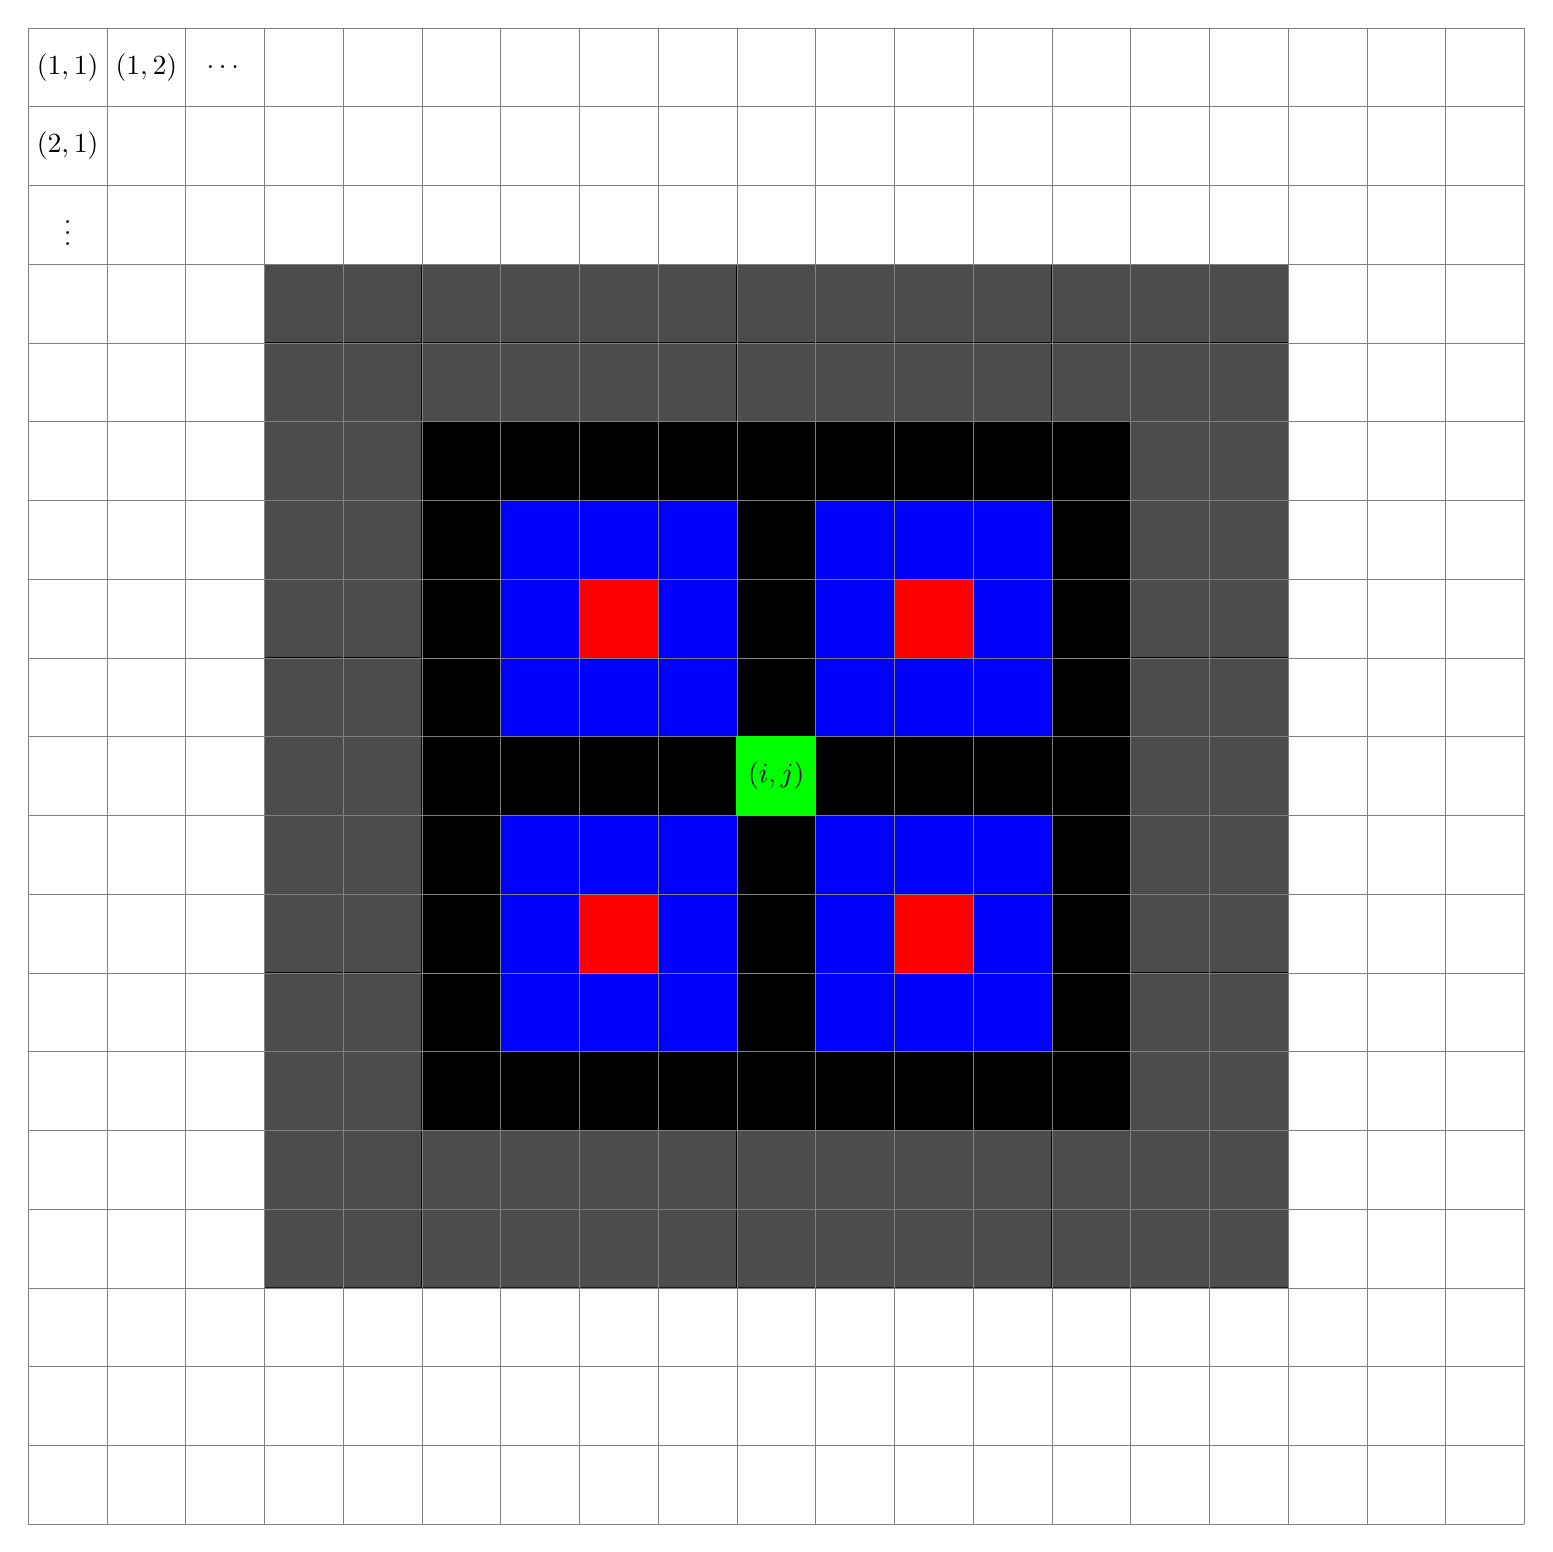
\begin{tikzpicture}
			\foreach \i in {-6, ..., 6}
				\foreach \j in {-6, ..., 6}
					\filldraw[black, opacity=0.7] (\i, \j) rectangle + (1, 1);
			\foreach \i in {-4, ..., 4}
				\foreach \j in {-4, ..., 4}
					\filldraw[black] (\i, \j) rectangle + (1, 1);
			\foreach \x in {(-3, -3), (-3, 1), (1, -3), (1, 1)}
				\filldraw[blue] \x rectangle + (3, 3);
			\foreach \x in {(-2, -2), (-2, 2), (2, -2), (2, 2)}
				\filldraw[red] \x rectangle + (1, 1);
			\draw[help lines, step=1] (-9, -9) grid (10, 10);
			\filldraw[green] (0, 0) rectangle + (1, 1);
			\node at (0.5, 0.5) {$(i, j)$};
			\node at (-8.5, 9.5) {$(1, 1)$};
			\node at (-7.5, 9.5) {$(1, 2)$};
			\node at (-6.5, 9.5) {$\dots$};
			\node at (-8.5, 8.5) {$(2, 1)$};
			\node at (-8.5, 7.5) {$\vdots$};
		\end{tikzpicture}
	}
	\caption{The black area are the pixels that contribute to $(\mathfrak{I} \circ \Psi_\varphi) \bullet \Psi_\varphi)(i, j)$. The blue squares are mutually independent. The red pixels are the pixels that we reduce the intersection in the proof to.}
	\label{fig: powerindependentpoints}
\end{figure}
		
		The sets $\bigcup_{\tilde{r}, \tilde{s} \in \Phi_\varphi} \{ \mathfrak{I}(i + k - \tilde{k} - r + \tilde{r}, j + \ell - \tilde{\ell} - s + \tilde{s}) = 0 \}$ are mutually independent for $r + \tilde{k}, s + \tilde{\ell} \in \{ - ( \varphi - 1 ), \varphi - 1 \}$ and fixed $k, \ell \in \Phi_\varphi$, see Figure \ref{fig: powerindependentpoints}. Thus we obtain
		\begin{align*}
			\mathbb{P}&_V\left( ((\mathfrak{I} \circ \Psi_\varphi) \bullet \Psi_\varphi)(i, j) = 0 \right) \\
			&\leq \sum_{k, \ell \in \Phi_\varphi} \mathbb{P}_V\left( \bigcap_{r + \tilde{k}, s + \tilde{\ell} \in \{ - ( \varphi - 1 ), \varphi - 1 \}} \bigcup_{\tilde{r}, \tilde{s} \in \Phi_\varphi} \{ \mathfrak{I}(i + k - \tilde{k} - r + \tilde{r}, j + \ell - \tilde{\ell} - s + \tilde{s}) = 0 \} \right) \\
			&= \sum_{k, \ell \in \Phi_\varphi} \prod_{r + \tilde{k}, s + \tilde{\ell} \in \{ - ( \varphi - 1 ), \varphi - 1 \}} \mathbb{P}_V\left( \bigcup_{\tilde{r}, \tilde{s} \in \Phi_\varphi} \{ \mathfrak{I}(i + k - \tilde{k} - r + \tilde{r}, j + \ell - \tilde{\ell} - s + \tilde{s}) = 0 \} \right).
		\end{align*}
		
		Again, by using sub-additivy, we get
		\begin{align*}
			\mathbb{P}&_V\left( ((\mathfrak{I} \circ \Psi_\varphi) \bullet \Psi_\varphi)(i, j) = 0 \right) \\
			&\leq \sum_{k, \ell \in \Phi_\varphi} \prod_{r + \tilde{k}, s + \tilde{\ell} \in \{ - ( \varphi - 1 ), \varphi - 1 \}} \mathbb{P}_V\left( \bigcup_{\tilde{r}, \tilde{s} \in \Phi_\varphi} \{ \mathfrak{I}(i + k - \tilde{k} - r + \tilde{r}, j + \ell - \tilde{\ell} - s + \tilde{s}) = 0 \} \right) \\
			&= \sum_{k, \ell \in \Phi_\varphi} \prod_{r + \tilde{k}, s + \tilde{\ell} \in \{ - ( \varphi - 1 ), \varphi - 1 \}} \sum_{\tilde{r}, \tilde{s} \in \Phi_\varphi} \mathbb{P}_V\left( \{ \mathfrak{I}(i + k - \tilde{k} - r + \tilde{r}, j + \ell - \tilde{\ell} - s + \tilde{s}) = 0 \} \right).
		\end{align*}
		
		We have assumed, that $(i, j) \in \Omega$ is such, that the alternative hypotheses $H_1(i + k - \tilde{k} - r + \tilde{r}, j + \ell - \tilde{\ell} - s + \tilde{s})$ are true for all $k, \ell, r, s, \tilde{k}, \tilde{\ell}, \tilde{r}, \tilde{s} \in \Phi_\varphi$. Using this assumption and the fact, that $\mathbb{P}_V\left( T(i, j) \leq t \right) \leq \beta$ for $\mathcal{H}_1(i, j)$ we obtain
		\begin{align*}
			\mathbb{P}&_V\left( ((\mathfrak{I} \circ \Psi_\varphi) \bullet \Psi_\varphi)(i, j) = 0 \right) \\
			&\leq \sum_{k, \ell \in \Phi_\varphi} \prod_{r + \tilde{k}, s + \tilde{\ell} \in \{ - ( \varphi - 1 ), \varphi - 1 \}} \sum_{\tilde{r}, \tilde{s} \in \Phi_\varphi} \mathbb{P}_V\left( \{ \mathfrak{I}(i + k - \tilde{k} - r + \tilde{r}, j + \ell - \tilde{\ell} - s + \tilde{s}) = 0 \} \right) \\
			&\leq \sum_{k, \ell \in \Phi_\varphi} \prod_{r + \tilde{k}, s + \tilde{\ell} \in \{ - ( \varphi - 1 ), \varphi - 1 \}} \sum_{\tilde{r}, \tilde{s} \in \Phi_\varphi} \beta \\
			&= \sum_{k, \ell \in \Phi_\varphi} \prod_{r + \tilde{k}, s + \tilde{\ell} \in \{ - ( \varphi - 1 ), \varphi - 1 \}} \varphi^2 \beta \\
			&= \sum_{k, \ell \in \Phi_\varphi} ( \varphi^2 \beta )^4 \\
			&= \varphi^2 ( \varphi^2 \beta )^4 \\
			&= \varphi^{10} \beta^4.
		\end{align*}
		
		This finishes the proof.
	\end{proof}
	
	\newpage
	
	\section{Simulations}\label{appendix: simulations}
	
	\begin{figure}[H]
	\centering
	\begin{subfigure}[t]{0.48\linewidth}
		\centering
		\begin{tikzpicture}
			\begin{axis}[
				legend pos=north west,
				legend style={nodes={scale=0.5, transform shape}},
				xlabel=Standard deviation $\sigma$,
				ylabel=False discovery rate,
				grid=both,
				minor grid style={gray!25},
				major grid style={gray!25},
				ymin=-0.05,
				ymax=1.05,
				width=\linewidth,
				no marks]
				\addplot[line width=1pt,dashed,color=blue] table[x=sigma,y=typeI,col sep=comma]{CSV/CSV_SinglePixel/normal/alpha0.05/phi3/background_corner.csv};
				\addlegendentry{Binarization}
				\addplot[line width=1pt,dashed,color=red] table[x=sigma,y=typeI_o,col sep=comma]{CSV/CSV_SinglePixel/normal/alpha0.05/phi3/background_corner.csv};
				\addlegendentry{Opening}
				\addplot[line width=1pt,dashed,color=gray] table[x=sigma,y=typeI_oc,col sep=comma]{CSV/CSV_SinglePixel/normal/alpha0.05/phi3/background_corner.csv};
				\addlegendentry{Opening \& Closing}
			\end{axis}
		\end{tikzpicture}
		\caption{Background pixel at the corner of the rROI.}
		\label{fig: normal_alpha0.05_phi3_background_corner}
	\end{subfigure}
	\hfill
	\begin{subfigure}[t]{0.48\linewidth}
		\centering
		\begin{tikzpicture}
			\begin{axis}[
				legend pos=north west,
				legend style={nodes={scale=0.5, transform shape}},
				xlabel=Standard deviation $\sigma$,
				ylabel=False rejection rate,
				grid=both,
				minor grid style={gray!25},
				major grid style={gray!25},
				ymin=-0.05,
				ymax=1.05,
				width=\linewidth,
				no marks]
				\addplot[line width=1pt,dashed,color=blue] table[x=sigma,y=typeII,col sep=comma]{CSV/CSV_SinglePixel/normal/alpha0.05/phi3/foreground_corner.csv};
				\addlegendentry{Binarization}
				\addplot[line width=1pt,dashed,color=red] table[x=sigma,y=typeII_o,col sep=comma]{CSV/CSV_SinglePixel/normal/alpha0.05/phi3/foreground_corner.csv};
				\addlegendentry{Opening}
				\addplot[line width=1pt,dashed,color=gray] table[x=sigma,y=typeII_oc,col sep=comma]{CSV/CSV_SinglePixel/normal/alpha0.05/phi3/foreground_corner.csv};
				\addlegendentry{Opening \& Closing}
			\end{axis}
		\end{tikzpicture}
		\caption{Foreground pixel at the corner of the rROI.}
		\label{fig: normal_alpha0.05_phi3_foreground_corner}
	\end{subfigure}
	\vfill
	\begin{subfigure}[t]{0.48\linewidth}
		\centering
		\begin{tikzpicture}
			\begin{axis}[
				legend pos=north west,
				legend style={nodes={scale=0.5, transform shape}},
				xlabel=Standard deviation $\sigma$,
				ylabel=False discovery rate,
				grid=both,
				minor grid style={gray!25},
				major grid style={gray!25},
				ymin=-0.05,
				ymax=1.05,
				width=\linewidth,
				no marks]
				\addplot[line width=1pt,dashed,color=blue] table[x=sigma,y=typeI,col sep=comma]{CSV/CSV_SinglePixel/normal/alpha0.05/phi3/background_edge.csv};
				\addlegendentry{Binarization}
				\addplot[line width=1pt,dashed,color=red] table[x=sigma,y=typeI_o,col sep=comma]{CSV/CSV_SinglePixel/normal/alpha0.05/phi3/background_edge.csv};
				\addlegendentry{Opening}
				\addplot[line width=1pt,dashed,color=gray] table[x=sigma,y=typeI_oc,col sep=comma]{CSV/CSV_SinglePixel/normal/alpha0.05/phi3/background_edge.csv};
				\addlegendentry{Opening \& Closing}
			\end{axis}
		\end{tikzpicture}
		\caption{Background pixel at the edge of the rROI.}
		\label{fig: normal_alpha0.05_phi3_background_edge}
	\end{subfigure}
	\hfill
	\begin{subfigure}[t]{0.48\linewidth}
		\centering
		\begin{tikzpicture}
			\begin{axis}[
				legend pos=north west,
				legend style={nodes={scale=0.5, transform shape}},
				xlabel=Standard deviation $\sigma$,
				ylabel=False rejection rate,
				grid=both,
				minor grid style={gray!25},
				major grid style={gray!25},
				ymin=-0.05,
				ymax=1.05,
				width=\linewidth,
				no marks]
				\addplot[line width=1pt,dashed,color=blue] table[x=sigma,y=typeII,col sep=comma]{CSV/CSV_SinglePixel/normal/alpha0.05/phi3/foreground_edge.csv};
				\addlegendentry{Binarization}
				\addplot[line width=1pt,dashed,color=red] table[x=sigma,y=typeII_o,col sep=comma]{CSV/CSV_SinglePixel/normal/alpha0.05/phi3/foreground_edge.csv};
				\addlegendentry{Opening}
				\addplot[line width=1pt,dashed,color=gray] table[x=sigma,y=typeII_oc,col sep=comma]{CSV/CSV_SinglePixel/normal/alpha0.05/phi3/foreground_edge.csv};
				\addlegendentry{Opening \& Closing}
			\end{axis}
		\end{tikzpicture}
		\caption{Foreground pixel at the edge of the rROI.}
		\label{fig: normal_alpha0.05_phi3_foreground_edge}
	\end{subfigure}
	\vfill
	\begin{subfigure}[t]{0.48\linewidth}
		\centering
		\begin{tikzpicture}
			\begin{axis}[
				legend pos=north west,
				legend style={nodes={scale=0.5, transform shape}},
				xlabel=Standard deviation $\sigma$,
				ylabel=False discovery rate,
				grid=both,
				minor grid style={gray!25},
				major grid style={gray!25},
				ymin=-0.05,
				ymax=1.05,
				width=\linewidth,
				no marks]
				\addplot[line width=1pt,dashed,color=blue] table[x=sigma,y=typeI,col sep=comma]{CSV/CSV_SinglePixel/normal/alpha0.05/phi3/background_free.csv};
				\addlegendentry{Binarization}
				\addplot[line width=1pt,dashed,color=red] table[x=sigma,y=typeI_o,col sep=comma]{CSV/CSV_SinglePixel/normal/alpha0.05/phi3/background_free.csv};
				\addlegendentry{Opening}
				\addplot[line width=1pt,dashed,color=gray] table[x=sigma,y=typeI_oc,col sep=comma]{CSV/CSV_SinglePixel/normal/alpha0.05/phi3/background_free.csv};
				\addlegendentry{Opening \& Closing}
			\end{axis}
		\end{tikzpicture}
		\caption{Background pixel surrounded by background.}
		\label{fig: normal_alpha0.05_phi3_background_free}
	\end{subfigure}
	\hfill
	\begin{subfigure}[t]{0.48\linewidth}
		\centering
		\begin{tikzpicture}
			\begin{axis}[
				legend pos=north west,
				legend style={nodes={scale=0.5, transform shape}},
				xlabel=Standard deviation $\sigma$,
				ylabel=False rejection rate,
				grid=both,
				minor grid style={gray!25},
				major grid style={gray!25},
				ymin=-0.05,
				ymax=1.05,
				width=\linewidth,
				no marks]
				\addplot[line width=1pt,dashed,color=blue] table[x=sigma,y=typeII,col sep=comma]{CSV/CSV_SinglePixel/normal/alpha0.05/phi3/foreground_free.csv};
				\addlegendentry{Binarization}
				\addplot[line width=1pt,dashed,color=red] table[x=sigma,y=typeII_o,col sep=comma]{CSV/CSV_SinglePixel/normal/alpha0.05/phi3/foreground_free.csv};
				\addlegendentry{Opening}
				\addplot[line width=1pt,dashed,color=gray] table[x=sigma,y=typeII_oc,col sep=comma]{CSV/CSV_SinglePixel/normal/alpha0.05/phi3/foreground_free.csv};
				\addlegendentry{Opening \& Closing}
			\end{axis}
		\end{tikzpicture}
		\caption{Foreground pixel surrounded by foreground.}
		\label{fig: normal_alpha0.05_phi3_foreground_free}
	\end{subfigure}
	\caption{Error rates after binarization, opening and closing. The $x$-axes display the standard deviation $\sigma$ and the $y$-axes the error rate. For each pixel type 1000 different noises were randomly generated $(\alpha = 0.05, \varphi = 3)$.}
	\label{fig: normal_alpha0.05_phi3}
\end{figure}
	
	\begin{figure}[H]
	\centering
	\begin{subfigure}[t]{0.48\linewidth}
		\centering
		\begin{tikzpicture}
			\begin{axis}[
				legend pos=north west,
				legend style={nodes={scale=0.5, transform shape}},
				xlabel=Standard deviation $\sigma$,
				ylabel=False discovery rate,
				grid=both,
				minor grid style={gray!25},
				major grid style={gray!25},
				ymin=-0.05,
				ymax=1.05,
				width=\linewidth,
				no marks]
				\addplot[line width=1pt,dashed,color=blue] table[x=sigma,y=typeI,col sep=comma]{CSV/CSV_SinglePixel/relaxed/alpha0.05/phi3/background_corner.csv};
				\addlegendentry{Binarization}
				\addplot[line width=1pt,dashed,color=red] table[x=sigma,y=typeI_o,col sep=comma]{CSV/CSV_SinglePixel/relaxed/alpha0.05/phi3/background_corner.csv};
				\addlegendentry{Opening}
				\addplot[line width=1pt,dashed,color=gray] table[x=sigma,y=typeI_oc,col sep=comma]{CSV/CSV_SinglePixel/relaxed/alpha0.05/phi3/background_corner.csv};
				\addlegendentry{Opening \& Closing}
			\end{axis}
		\end{tikzpicture}
		\caption{Background pixel at the corner of the rROI.}
		\label{fig: relaxed_alpha0.05_phi3_background_corner}
	\end{subfigure}
	\hfill
	\begin{subfigure}[t]{0.48\linewidth}
		\centering
		\begin{tikzpicture}
			\begin{axis}[
				legend pos=north west,
				legend style={nodes={scale=0.5, transform shape}},
				xlabel=Standard deviation $\sigma$,
				ylabel=False rejection rate,
				grid=both,
				minor grid style={gray!25},
				major grid style={gray!25},
				ymin=-0.05,
				ymax=1.05,
				width=\linewidth,
				no marks]
				\addplot[line width=1pt,dashed,color=blue] table[x=sigma,y=typeII,col sep=comma]{CSV/CSV_SinglePixel/relaxed/alpha0.05/phi3/foreground_corner.csv};
				\addlegendentry{Binarization}
				\addplot[line width=1pt,dashed,color=red] table[x=sigma,y=typeII_o,col sep=comma]{CSV/CSV_SinglePixel/relaxed/alpha0.05/phi3/foreground_corner.csv};
				\addlegendentry{Opening}
				\addplot[line width=1pt,dashed,color=gray] table[x=sigma,y=typeII_oc,col sep=comma]{CSV/CSV_SinglePixel/relaxed/alpha0.05/phi3/foreground_corner.csv};
				\addlegendentry{Opening \& Closing}
			\end{axis}
		\end{tikzpicture}
		\caption{Foreground pixel at the corner of the rROI.}
		\label{fig: relaxed_alpha0.05_phi3_foreground_corner}
	\end{subfigure}
	\vfill
	\begin{subfigure}[t]{0.48\linewidth}
		\centering
		\begin{tikzpicture}
			\begin{axis}[
				legend pos=north west,
				legend style={nodes={scale=0.5, transform shape}},
				xlabel=Standard deviation $\sigma$,
				ylabel=False discovery rate,
				grid=both,
				minor grid style={gray!25},
				major grid style={gray!25},
				ymin=-0.05,
				ymax=1.05,
				width=\linewidth,
				no marks]
				\addplot[line width=1pt,dashed,color=blue] table[x=sigma,y=typeI,col sep=comma]{CSV/CSV_SinglePixel/relaxed/alpha0.05/phi3/background_edge.csv};
				\addlegendentry{Binarization}
				\addplot[line width=1pt,dashed,color=red] table[x=sigma,y=typeI_o,col sep=comma]{CSV/CSV_SinglePixel/relaxed/alpha0.05/phi3/background_edge.csv};
				\addlegendentry{Opening}
				\addplot[line width=1pt,dashed,color=gray] table[x=sigma,y=typeI_oc,col sep=comma]{CSV/CSV_SinglePixel/relaxed/alpha0.05/phi3/background_edge.csv};
				\addlegendentry{Opening \& Closing}
			\end{axis}
		\end{tikzpicture}
		\caption{Background pixel at the edge of the rROI.}
		\label{fig: relaxed_alpha0.05_phi3_background_edge}
	\end{subfigure}
	\hfill
	\begin{subfigure}[t]{0.48\linewidth}
		\centering
		\begin{tikzpicture}
			\begin{axis}[
				legend pos=north west,
				legend style={nodes={scale=0.5, transform shape}},
				xlabel=Standard deviation $\sigma$,
				ylabel=False rejection rate,
				grid=both,
				minor grid style={gray!25},
				major grid style={gray!25},
				ymin=-0.05,
				ymax=1.05,
				width=\linewidth,
				no marks]
				\addplot[line width=1pt,dashed,color=blue] table[x=sigma,y=typeII,col sep=comma]{CSV/CSV_SinglePixel/relaxed/alpha0.05/phi3/foreground_edge.csv};
				\addlegendentry{Binarization}
				\addplot[line width=1pt,dashed,color=red] table[x=sigma,y=typeII_o,col sep=comma]{CSV/CSV_SinglePixel/relaxed/alpha0.05/phi3/foreground_edge.csv};
				\addlegendentry{Opening}
				\addplot[line width=1pt,dashed,color=gray] table[x=sigma,y=typeII_oc,col sep=comma]{CSV/CSV_SinglePixel/relaxed/alpha0.05/phi3/foreground_edge.csv};
				\addlegendentry{Opening \& Closing}
			\end{axis}
		\end{tikzpicture}
		\caption{Foreground pixel at the edge of the rROI.}
		\label{fig: relaxed_alpha0.05_phi3_foreground_edge}
	\end{subfigure}
	\vfill
	\begin{subfigure}[t]{0.48\linewidth}
		\centering
		\begin{tikzpicture}
			\begin{axis}[
				legend pos=north west,
				legend style={nodes={scale=0.5, transform shape}},
				xlabel=Standard deviation $\sigma$,
				ylabel=False discovery rate,
				grid=both,
				minor grid style={gray!25},
				major grid style={gray!25},
				ymin=-0.05,
				ymax=1.05,
				width=\linewidth,
				no marks]
				\addplot[line width=1pt,dashed,color=blue] table[x=sigma,y=typeI,col sep=comma]{CSV/CSV_SinglePixel/relaxed/alpha0.05/phi3/background_free.csv};
				\addlegendentry{Binarization}
				\addplot[line width=1pt,dashed,color=red] table[x=sigma,y=typeI_o,col sep=comma]{CSV/CSV_SinglePixel/relaxed/alpha0.05/phi3/background_free.csv};
				\addlegendentry{Opening}
				\addplot[line width=1pt,dashed,color=gray] table[x=sigma,y=typeI_oc,col sep=comma]{CSV/CSV_SinglePixel/relaxed/alpha0.05/phi3/background_free.csv};
				\addlegendentry{Opening \& Closing}
			\end{axis}
		\end{tikzpicture}
		\caption{Background pixel surrounded by background.}
		\label{fig: relaxed_alpha0.05_phi3_background_free}
	\end{subfigure}
	\hfill
	\begin{subfigure}[t]{0.48\linewidth}
		\centering
		\begin{tikzpicture}
			\begin{axis}[
				legend pos=north west,
				legend style={nodes={scale=0.5, transform shape}},
				xlabel=Standard deviation $\sigma$,
				ylabel=False rejection rate,
				grid=both,
				minor grid style={gray!25},
				major grid style={gray!25},
				ymin=-0.05,
				ymax=1.05,
				width=\linewidth,
				no marks]
				\addplot[line width=1pt,dashed,color=blue] table[x=sigma,y=typeII,col sep=comma]{CSV/CSV_SinglePixel/relaxed/alpha0.05/phi3/foreground_free.csv};
				\addlegendentry{Binarization}
				\addplot[line width=1pt,dashed,color=red] table[x=sigma,y=typeII_o,col sep=comma]{CSV/CSV_SinglePixel/relaxed/alpha0.05/phi3/foreground_free.csv};
				\addlegendentry{Opening}
				\addplot[line width=1pt,dashed,color=gray] table[x=sigma,y=typeII_oc,col sep=comma]{CSV/CSV_SinglePixel/relaxed/alpha0.05/phi3/foreground_free.csv};
				\addlegendentry{Opening \& Closing}
			\end{axis}
		\end{tikzpicture}
		\caption{Foreground pixel surrounded by foreground.}
		\label{fig: relaxed_alpha0.05_phi3_foreground_free}
	\end{subfigure}
	\caption{Error rates after binarization, opening and closing. The $x$-axes display the standard deviation $\sigma$ and the $y$-axes the error rate. For each pixel type 1000 different noises were randomly generated $\left( \tilde{\alpha} = \left( \frac{0.05}{3^3} \right)^{\frac{2}{3 + 1}}, \varphi = 3 \right)$.}
	\label{fig: relaxed_alpha0.05_phi3}
\end{figure}
	
	\begin{figure}[H]
	\centering
	\begin{subfigure}[t]{0.48\linewidth}
		\centering
		\begin{tikzpicture}
			\begin{axis}[
				legend pos=north west,
				legend style={nodes={scale=0.5, transform shape}},
				xlabel=Standard deviation $\sigma$,
				ylabel=False discovery rate,
				grid=both,
				minor grid style={gray!25},
				major grid style={gray!25},
				ymin=-0.05,
				ymax=1.05,
				width=\linewidth,
				no marks]
				\addplot[line width=1pt,dashed,color=blue] table[x=sigma,y=typeI,col sep=comma]{CSV/CSV_SinglePixel/normal/alpha0.05/phi7/background_corner.csv};
				\addlegendentry{Binarization}
				\addplot[line width=1pt,dashed,color=red] table[x=sigma,y=typeI_o,col sep=comma]{CSV/CSV_SinglePixel/normal/alpha0.05/phi7/background_corner.csv};
				\addlegendentry{Opening}
				\addplot[line width=1pt,dashed,color=gray] table[x=sigma,y=typeI_oc,col sep=comma]{CSV/CSV_SinglePixel/normal/alpha0.05/phi7/background_corner.csv};
				\addlegendentry{Opening \& Closing}
			\end{axis}
		\end{tikzpicture}
		\caption{Background pixel at the corner of the rROI.}
		\label{fig: normal_alpha0.05_phi7_background_corner}
	\end{subfigure}
	\hfill
	\begin{subfigure}[t]{0.48\linewidth}
		\centering
		\begin{tikzpicture}
			\begin{axis}[
				legend pos=north west,
				legend style={nodes={scale=0.5, transform shape}},
				xlabel=Standard deviation $\sigma$,
				ylabel=False rejection rate,
				grid=both,
				minor grid style={gray!25},
				major grid style={gray!25},
				ymin=-0.05,
				ymax=1.05,
				width=\linewidth,
				no marks]
				\addplot[line width=1pt,dashed,color=blue] table[x=sigma,y=typeII,col sep=comma]{CSV/CSV_SinglePixel/normal/alpha0.05/phi7/foreground_corner.csv};
				\addlegendentry{Binarization}
				\addplot[line width=1pt,dashed,color=red] table[x=sigma,y=typeII_o,col sep=comma]{CSV/CSV_SinglePixel/normal/alpha0.05/phi7/foreground_corner.csv};
				\addlegendentry{Opening}
				\addplot[line width=1pt,dashed,color=gray] table[x=sigma,y=typeII_oc,col sep=comma]{CSV/CSV_SinglePixel/normal/alpha0.05/phi7/foreground_corner.csv};
				\addlegendentry{Opening \& Closing}
			\end{axis}
		\end{tikzpicture}
		\caption{Foreground pixel at the corner of the rROI.}
		\label{fig: normal_alpha0.05_phi7_foreground_corner}
	\end{subfigure}
	\vfill
	\begin{subfigure}[t]{0.48\linewidth}
		\centering
		\begin{tikzpicture}
			\begin{axis}[
				legend pos=north west,
				legend style={nodes={scale=0.5, transform shape}},
				xlabel=Standard deviation $\sigma$,
				ylabel=False discovery rate,
				grid=both,
				minor grid style={gray!25},
				major grid style={gray!25},
				ymin=-0.05,
				ymax=1.05,
				width=\linewidth,
				no marks]
				\addplot[line width=1pt,dashed,color=blue] table[x=sigma,y=typeI,col sep=comma]{CSV/CSV_SinglePixel/normal/alpha0.05/phi7/background_edge.csv};
				\addlegendentry{Binarization}
				\addplot[line width=1pt,dashed,color=red] table[x=sigma,y=typeI_o,col sep=comma]{CSV/CSV_SinglePixel/normal/alpha0.05/phi7/background_edge.csv};
				\addlegendentry{Opening}
				\addplot[line width=1pt,dashed,color=gray] table[x=sigma,y=typeI_oc,col sep=comma]{CSV/CSV_SinglePixel/normal/alpha0.05/phi7/background_edge.csv};
				\addlegendentry{Opening \& Closing}
			\end{axis}
		\end{tikzpicture}
		\caption{Background pixel at the edge of the rROI.}
		\label{fig: normal_alpha0.05_phi7_background_edge}
	\end{subfigure}
	\hfill
	\begin{subfigure}[t]{0.48\linewidth}
		\centering
		\begin{tikzpicture}
			\begin{axis}[
				legend pos=north west,
				legend style={nodes={scale=0.5, transform shape}},
				xlabel=Standard deviation $\sigma$,
				ylabel=False rejection rate,
				grid=both,
				minor grid style={gray!25},
				major grid style={gray!25},
				ymin=-0.05,
				ymax=1.05,
				width=\linewidth,
				no marks]
				\addplot[line width=1pt,dashed,color=blue] table[x=sigma,y=typeII,col sep=comma]{CSV/CSV_SinglePixel/normal/alpha0.05/phi7/foreground_edge.csv};
				\addlegendentry{Binarization}
				\addplot[line width=1pt,dashed,color=red] table[x=sigma,y=typeII_o,col sep=comma]{CSV/CSV_SinglePixel/normal/alpha0.05/phi7/foreground_edge.csv};
				\addlegendentry{Opening}
				\addplot[line width=1pt,dashed,color=gray] table[x=sigma,y=typeII_oc,col sep=comma]{CSV/CSV_SinglePixel/normal/alpha0.05/phi7/foreground_edge.csv};
				\addlegendentry{Opening \& Closing}
			\end{axis}
		\end{tikzpicture}
		\caption{Foreground pixel at the edge of the rROI.}
		\label{fig: normal_alpha0.05_phi7_foreground_edge}
	\end{subfigure}
	\vfill
	\begin{subfigure}[t]{0.48\linewidth}
		\centering
		\begin{tikzpicture}
			\begin{axis}[
				legend pos=north west,
				legend style={nodes={scale=0.5, transform shape}},
				xlabel=Standard deviation $\sigma$,
				ylabel=False discovery rate,
				grid=both,
				minor grid style={gray!25},
				major grid style={gray!25},
				ymin=-0.05,
				ymax=1.05,
				width=\linewidth,
				no marks]
				\addplot[line width=1pt,dashed,color=blue] table[x=sigma,y=typeI,col sep=comma]{CSV/CSV_SinglePixel/normal/alpha0.05/phi7/background_free.csv};
				\addlegendentry{Binarization}
				\addplot[line width=1pt,dashed,color=red] table[x=sigma,y=typeI_o,col sep=comma]{CSV/CSV_SinglePixel/normal/alpha0.05/phi7/background_free.csv};
				\addlegendentry{Opening}
				\addplot[line width=1pt,dashed,color=gray] table[x=sigma,y=typeI_oc,col sep=comma]{CSV/CSV_SinglePixel/normal/alpha0.05/phi7/background_free.csv};
				\addlegendentry{Opening \& Closing}
			\end{axis}
		\end{tikzpicture}
		\caption{Background pixel surrounded by background.}
		\label{fig: normal_alpha0.05_phi7_background_free}
	\end{subfigure}
	\hfill
	\begin{subfigure}[t]{0.48\linewidth}
		\centering
		\begin{tikzpicture}
			\begin{axis}[
				legend pos=north west,
				legend style={nodes={scale=0.5, transform shape}},
				xlabel=Standard deviation $\sigma$,
				ylabel=False rejection rate,
				grid=both,
				minor grid style={gray!25},
				major grid style={gray!25},
				ymin=-0.05,
				ymax=1.05,
				width=\linewidth,
				no marks]
				\addplot[line width=1pt,dashed,color=blue] table[x=sigma,y=typeII,col sep=comma]{CSV/CSV_SinglePixel/normal/alpha0.05/phi7/foreground_free.csv};
				\addlegendentry{Binarization}
				\addplot[line width=1pt,dashed,color=red] table[x=sigma,y=typeII_o,col sep=comma]{CSV/CSV_SinglePixel/normal/alpha0.05/phi7/foreground_free.csv};
				\addlegendentry{Opening}
				\addplot[line width=1pt,dashed,color=gray] table[x=sigma,y=typeII_oc,col sep=comma]{CSV/CSV_SinglePixel/normal/alpha0.05/phi7/foreground_free.csv};
				\addlegendentry{Opening \& Closing}
			\end{axis}
		\end{tikzpicture}
		\caption{Foreground pixel surrounded by foreground.}
		\label{fig: normal_alpha0.05_phi7_foreground_free}
	\end{subfigure}
	\caption{Error rates after binarization, opening and closing. The $x$-axes display the standard deviation $\sigma$ and the $y$-axes the error rate. For each pixel type 1000 different noises were randomly generated $(\alpha = 0.05, \varphi = 7)$.}
	\label{fig: normal_alpha0.05_phi7}
\end{figure}
	
	\begin{figure}[H]
	\centering
	\begin{subfigure}[t]{0.48\linewidth}
		\centering
		\begin{tikzpicture}
			\begin{axis}[
				legend pos=north west,
				legend style={nodes={scale=0.5, transform shape}},
				xlabel=Standard deviation $\sigma$,
				ylabel=False discovery rate,
				grid=both,
				minor grid style={gray!25},
				major grid style={gray!25},
				ymin=-0.05,
				ymax=1.05,
				width=\linewidth,
				no marks]
				\addplot[line width=1pt,dashed,color=blue] table[x=sigma,y=typeI,col sep=comma]{CSV/CSV_SinglePixel/relaxed/alpha0.05/phi7/background_corner.csv};
				\addlegendentry{Binarization}
				\addplot[line width=1pt,dashed,color=red] table[x=sigma,y=typeI_o,col sep=comma]{CSV/CSV_SinglePixel/relaxed/alpha0.05/phi7/background_corner.csv};
				\addlegendentry{Opening}
				\addplot[line width=1pt,dashed,color=gray] table[x=sigma,y=typeI_oc,col sep=comma]{CSV/CSV_SinglePixel/relaxed/alpha0.05/phi7/background_corner.csv};
				\addlegendentry{Opening \& Closing}
			\end{axis}
		\end{tikzpicture}
		\caption{Background pixel at the corner of the rROI.}
		\label{fig: relaxed_alpha0.05_phi7_background_corner}
	\end{subfigure}
	\hfill
	\begin{subfigure}[t]{0.48\linewidth}
		\centering
		\begin{tikzpicture}
			\begin{axis}[
				legend pos=north west,
				legend style={nodes={scale=0.5, transform shape}},
				xlabel=Standard deviation $\sigma$,
				ylabel=False rejection rate,
				grid=both,
				minor grid style={gray!25},
				major grid style={gray!25},
				ymin=-0.05,
				ymax=1.05,
				width=\linewidth,
				no marks]
				\addplot[line width=1pt,dashed,color=blue] table[x=sigma,y=typeII,col sep=comma]{CSV/CSV_SinglePixel/relaxed/alpha0.05/phi7/foreground_corner.csv};
				\addlegendentry{Binarization}
				\addplot[line width=1pt,dashed,color=red] table[x=sigma,y=typeII_o,col sep=comma]{CSV/CSV_SinglePixel/relaxed/alpha0.05/phi7/foreground_corner.csv};
				\addlegendentry{Opening}
				\addplot[line width=1pt,dashed,color=gray] table[x=sigma,y=typeII_oc,col sep=comma]{CSV/CSV_SinglePixel/relaxed/alpha0.05/phi7/foreground_corner.csv};
				\addlegendentry{Opening \& Closing}
			\end{axis}
		\end{tikzpicture}
		\caption{Foreground pixel at the corner of the rROI.}
		\label{fig: relaxed_alpha0.05_phi7_foreground_corner}
	\end{subfigure}
	\vfill
	\begin{subfigure}[t]{0.48\linewidth}
		\centering
		\begin{tikzpicture}
			\begin{axis}[
				legend pos=north west,
				legend style={nodes={scale=0.5, transform shape}},
				xlabel=Standard deviation $\sigma$,
				ylabel=False discovery rate,
				grid=both,
				minor grid style={gray!25},
				major grid style={gray!25},
				ymin=-0.05,
				ymax=1.05,
				width=\linewidth,
				no marks]
				\addplot[line width=1pt,dashed,color=blue] table[x=sigma,y=typeI,col sep=comma]{CSV/CSV_SinglePixel/relaxed/alpha0.05/phi7/background_edge.csv};
				\addlegendentry{Binarization}
				\addplot[line width=1pt,dashed,color=red] table[x=sigma,y=typeI_o,col sep=comma]{CSV/CSV_SinglePixel/relaxed/alpha0.05/phi7/background_edge.csv};
				\addlegendentry{Opening}
				\addplot[line width=1pt,dashed,color=gray] table[x=sigma,y=typeI_oc,col sep=comma]{CSV/CSV_SinglePixel/relaxed/alpha0.05/phi7/background_edge.csv};
				\addlegendentry{Opening \& Closing}
			\end{axis}
		\end{tikzpicture}
		\caption{Background pixel at the edge of the rROI.}
		\label{fig: relaxed_alpha0.05_phi7_background_edge}
	\end{subfigure}
	\hfill
	\begin{subfigure}[t]{0.48\linewidth}
		\centering
		\begin{tikzpicture}
			\begin{axis}[
				legend pos=north west,
				legend style={nodes={scale=0.5, transform shape}},
				xlabel=Standard deviation $\sigma$,
				ylabel=False rejection rate,
				grid=both,
				minor grid style={gray!25},
				major grid style={gray!25},
				ymin=-0.05,
				ymax=1.05,
				width=\linewidth,
				no marks]
				\addplot[line width=1pt,dashed,color=blue] table[x=sigma,y=typeII,col sep=comma]{CSV/CSV_SinglePixel/relaxed/alpha0.05/phi7/foreground_edge.csv};
				\addlegendentry{Binarization}
				\addplot[line width=1pt,dashed,color=red] table[x=sigma,y=typeII_o,col sep=comma]{CSV/CSV_SinglePixel/relaxed/alpha0.05/phi7/foreground_edge.csv};
				\addlegendentry{Opening}
				\addplot[line width=1pt,dashed,color=gray] table[x=sigma,y=typeII_oc,col sep=comma]{CSV/CSV_SinglePixel/relaxed/alpha0.05/phi7/foreground_edge.csv};
				\addlegendentry{Opening \& Closing}
			\end{axis}
		\end{tikzpicture}
		\caption{Foreground pixel at the edge of the rROI.}
		\label{fig: relaxed_alpha0.05_phi7_foreground_edge}
	\end{subfigure}
	\vfill
	\begin{subfigure}[t]{0.48\linewidth}
		\centering
		\begin{tikzpicture}
			\begin{axis}[
				legend pos=north west,
				legend style={nodes={scale=0.5, transform shape}},
				xlabel=Standard deviation $\sigma$,
				ylabel=False discovery rate,
				grid=both,
				minor grid style={gray!25},
				major grid style={gray!25},
				ymin=-0.05,
				ymax=1.05,
				width=\linewidth,
				no marks]
				\addplot[line width=1pt,dashed,color=blue] table[x=sigma,y=typeI,col sep=comma]{CSV/CSV_SinglePixel/relaxed/alpha0.05/phi7/background_free.csv};
				\addlegendentry{Binarization}
				\addplot[line width=1pt,dashed,color=red] table[x=sigma,y=typeI_o,col sep=comma]{CSV/CSV_SinglePixel/relaxed/alpha0.05/phi7/background_free.csv};
				\addlegendentry{Opening}
				\addplot[line width=1pt,dashed,color=gray] table[x=sigma,y=typeI_oc,col sep=comma]{CSV/CSV_SinglePixel/relaxed/alpha0.05/phi7/background_free.csv};
				\addlegendentry{Opening \& Closing}
			\end{axis}
		\end{tikzpicture}
		\caption{Background pixel surrounded by background.}
		\label{fig: relaxed_alpha0.05_phi7_background_free}
	\end{subfigure}
	\hfill
	\begin{subfigure}[t]{0.48\linewidth}
		\centering
		\begin{tikzpicture}
			\begin{axis}[
				legend pos=north west,
				legend style={nodes={scale=0.5, transform shape}},
				xlabel=Standard deviation $\sigma$,
				ylabel=False rejection rate,
				grid=both,
				minor grid style={gray!25},
				major grid style={gray!25},
				ymin=-0.05,
				ymax=1.05,
				width=\linewidth,
				no marks]
				\addplot[line width=1pt,dashed,color=blue] table[x=sigma,y=typeII,col sep=comma]{CSV/CSV_SinglePixel/relaxed/alpha0.05/phi7/foreground_free.csv};
				\addlegendentry{Binarization}
				\addplot[line width=1pt,dashed,color=red] table[x=sigma,y=typeII_o,col sep=comma]{CSV/CSV_SinglePixel/relaxed/alpha0.05/phi7/foreground_free.csv};
				\addlegendentry{Opening}
				\addplot[line width=1pt,dashed,color=gray] table[x=sigma,y=typeII_oc,col sep=comma]{CSV/CSV_SinglePixel/relaxed/alpha0.05/phi7/foreground_free.csv};
				\addlegendentry{Opening \& Closing}
			\end{axis}
		\end{tikzpicture}
		\caption{Foreground pixel surrounded by foreground.}
		\label{fig: relaxed_alpha0.05_phi7_foreground_free}
	\end{subfigure}
	\caption{Error rates after binarization, opening and closing. The $x$-axes display the standard deviation $\sigma$ and the $y$-axes the error rate. For each pixel type 1000 different noises were randomly generated $\left( \tilde{\alpha} = \left( \frac{0.05}{7^3} \right)^{\frac{2}{7 + 1}}, \varphi = 7 \right)$.}
	\label{fig: relaxed_alpha0.05_phi7}
\end{figure}
	
	\begin{figure}[H]
	\centering
	\begin{subfigure}[t]{0.48\linewidth}
		\centering
		\begin{tikzpicture}
			\begin{axis}[
				legend pos=north west,
				legend style={nodes={scale=0.5, transform shape}},
				xlabel=Standard deviation $\sigma$,
				ylabel=False positive rate,
				grid=both,
				minor grid style={gray!25},
				major grid style={gray!25},
				ymin=-0.05,
				ymax=1.05,
				width=\linewidth,
				no marks]
				\addplot[line width=1pt,dashed,color=blue] table[x=sigma,y=typeI,col sep=comma]{CSV/CSV_SinglePixel/normal/alpha0.05/phi99/background_corner.csv};
				\addlegendentry{Binarization}
				\addplot[line width=1pt,dashed,color=red] table[x=sigma,y=typeI_o,col sep=comma]{CSV/CSV_SinglePixel/normal/alpha0.05/phi99/background_corner.csv};
				\addlegendentry{Opening}
				\addplot[line width=1pt,dashed,color=gray] table[x=sigma,y=typeI_oc,col sep=comma]{CSV/CSV_SinglePixel/normal/alpha0.05/phi99/background_corner.csv};
				\addlegendentry{Opening \& Closing}
			\end{axis}
		\end{tikzpicture}
		\caption{Background pixel at the corner of the rROI.}
		\label{fig: normal_alpha0.05_phi99_background_corner}
	\end{subfigure}
	\hfill
	\begin{subfigure}[t]{0.48\linewidth}
		\centering
		\begin{tikzpicture}
			\begin{axis}[
				legend pos=north west,
				legend style={nodes={scale=0.5, transform shape}},
				xlabel=Standard deviation $\sigma$,
				ylabel=False negative rate,
				grid=both,
				minor grid style={gray!25},
				major grid style={gray!25},
				ymin=-0.05,
				ymax=1.05,
				width=\linewidth,
				no marks]
				\addplot[line width=1pt,dashed,color=blue] table[x=sigma,y=typeII,col sep=comma]{CSV/CSV_SinglePixel/normal/alpha0.05/phi99/foreground_corner.csv};
				\addlegendentry{Binarization}
				\addplot[line width=1pt,dashed,color=red] table[x=sigma,y=typeII_o,col sep=comma]{CSV/CSV_SinglePixel/normal/alpha0.05/phi99/foreground_corner.csv};
				\addlegendentry{Opening}
				\addplot[line width=1pt,dashed,color=gray] table[x=sigma,y=typeII_oc,col sep=comma]{CSV/CSV_SinglePixel/normal/alpha0.05/phi99/foreground_corner.csv};
				\addlegendentry{Opening \& Closing}
			\end{axis}
		\end{tikzpicture}
		\caption{Foreground pixel at the corner of the rROI.}
		\label{fig: normal_alpha0.05_phi99_foreground_corner}
	\end{subfigure}
	\vfill
	\begin{subfigure}[t]{0.48\linewidth}
		\centering
		\begin{tikzpicture}
			\begin{axis}[
				legend pos=north west,
				legend style={nodes={scale=0.5, transform shape}},
				xlabel=Standard deviation $\sigma$,
				ylabel=False positive rate,
				grid=both,
				minor grid style={gray!25},
				major grid style={gray!25},
				ymin=-0.05,
				ymax=1.05,
				width=\linewidth,
				no marks]
				\addplot[line width=1pt,dashed,color=blue] table[x=sigma,y=typeI,col sep=comma]{CSV/CSV_SinglePixel/normal/alpha0.05/phi99/background_edge.csv};
				\addlegendentry{Binarization}
				\addplot[line width=1pt,dashed,color=red] table[x=sigma,y=typeI_o,col sep=comma]{CSV/CSV_SinglePixel/normal/alpha0.05/phi99/background_edge.csv};
				\addlegendentry{Opening}
				\addplot[line width=1pt,dashed,color=gray] table[x=sigma,y=typeI_oc,col sep=comma]{CSV/CSV_SinglePixel/normal/alpha0.05/phi99/background_edge.csv};
				\addlegendentry{Opening \& Closing}
			\end{axis}
		\end{tikzpicture}
		\caption{Background pixel at the edge of the rROI.}
		\label{fig: normal_alpha0.05_phi99_background_edge}
	\end{subfigure}
	\hfill
	\begin{subfigure}[t]{0.48\linewidth}
		\centering
		\begin{tikzpicture}
			\begin{axis}[
				legend pos=north west,
				legend style={nodes={scale=0.5, transform shape}},
				xlabel=Standard deviation $\sigma$,
				ylabel=False negative rate,
				grid=both,
				minor grid style={gray!25},
				major grid style={gray!25},
				ymin=-0.05,
				ymax=1.05,
				width=\linewidth,
				no marks]
				\addplot[line width=1pt,dashed,color=blue] table[x=sigma,y=typeII,col sep=comma]{CSV/CSV_SinglePixel/normal/alpha0.05/phi99/foreground_edge.csv};
				\addlegendentry{Binarization}
				\addplot[line width=1pt,dashed,color=red] table[x=sigma,y=typeII_o,col sep=comma]{CSV/CSV_SinglePixel/normal/alpha0.05/phi99/foreground_edge.csv};
				\addlegendentry{Opening}
				\addplot[line width=1pt,dashed,color=gray] table[x=sigma,y=typeII_oc,col sep=comma]{CSV/CSV_SinglePixel/normal/alpha0.05/phi99/foreground_edge.csv};
				\addlegendentry{Opening \& Closing}
			\end{axis}
		\end{tikzpicture}
		\caption{Foreground pixel at the edge of the rROI.}
		\label{fig: normal_alpha0.05_phi99_foreground_edge}
	\end{subfigure}
	\vfill
	\begin{subfigure}[t]{0.48\linewidth}
		\centering
		\begin{tikzpicture}
			\begin{axis}[
				legend pos=north west,
				legend style={nodes={scale=0.5, transform shape}},
				xlabel=Standard deviation $\sigma$,
				ylabel=False positive rate,
				grid=both,
				minor grid style={gray!25},
				major grid style={gray!25},
				ymin=-0.05,
				ymax=1.05,
				width=\linewidth,
				no marks]
				\addplot[line width=1pt,dashed,color=blue] table[x=sigma,y=typeI,col sep=comma]{CSV/CSV_SinglePixel/normal/alpha0.05/phi99/background_free.csv};
				\addlegendentry{Binarization}
				\addplot[line width=1pt,dashed,color=red] table[x=sigma,y=typeI_o,col sep=comma]{CSV/CSV_SinglePixel/normal/alpha0.05/phi99/background_free.csv};
				\addlegendentry{Opening}
				\addplot[line width=1pt,dashed,color=gray] table[x=sigma,y=typeI_oc,col sep=comma]{CSV/CSV_SinglePixel/normal/alpha0.05/phi99/background_free.csv};
				\addlegendentry{Opening \& Closing}
			\end{axis}
		\end{tikzpicture}
		\caption{Background pixel surrounded by background.}
		\label{fig: normal_alpha0.05_phi99_background_free}
	\end{subfigure}
	\hfill
	\begin{subfigure}[t]{0.48\linewidth}
		\centering
		\begin{tikzpicture}
			\begin{axis}[
				legend pos=north west,
				legend style={nodes={scale=0.5, transform shape}},
				xlabel=Standard deviation $\sigma$,
				ylabel=False negative rate,
				grid=both,
				minor grid style={gray!25},
				major grid style={gray!25},
				ymin=-0.05,
				ymax=1.05,
				width=\linewidth,
				no marks]
				\addplot[line width=1pt,dashed,color=blue] table[x=sigma,y=typeII,col sep=comma]{CSV/CSV_SinglePixel/normal/alpha0.05/phi99/foreground_free.csv};
				\addlegendentry{Binarization}
				\addplot[line width=1pt,dashed,color=red] table[x=sigma,y=typeII_o,col sep=comma]{CSV/CSV_SinglePixel/normal/alpha0.05/phi99/foreground_free.csv};
				\addlegendentry{Opening}
				\addplot[line width=1pt,dashed,color=gray] table[x=sigma,y=typeII_oc,col sep=comma]{CSV/CSV_SinglePixel/normal/alpha0.05/phi99/foreground_free.csv};
				\addlegendentry{Opening \& Closing}
			\end{axis}
		\end{tikzpicture}
		\caption{Foreground pixel surrounded by foreground.}
		\label{fig: normal_alpha0.05_phi99_foreground_free}
	\end{subfigure}
	\caption{Error rates after binarization, opening and closing. The $x$-axes display the standard deviation $\sigma$ and the $y$-axes the error rate. For each pixel type 1000 different noises were randomly generated $(\alpha = 0.05, \varphi = 99)$.}
	\label{fig: normal_alpha0.05_phi99}
\end{figure}
	
	\begin{figure}[H]
	\centering
	\begin{subfigure}[t]{0.48\linewidth}
		\centering
		\begin{tikzpicture}
			\begin{axis}[
				legend pos=north west,
				legend style={nodes={scale=0.5, transform shape}},
				xlabel=Standard deviation $\sigma$,
				ylabel=False discovery rate,
				grid=both,
				minor grid style={gray!25},
				major grid style={gray!25},
				ymin=-0.05,
				ymax=1.05,
				width=\linewidth,
				no marks]
				\addplot[line width=1pt,dashed,color=blue] table[x=sigma,y=typeI,col sep=comma]{CSV/CSV_SinglePixel/relaxed/alpha0.05/phi99/background_corner.csv};
				\addlegendentry{Binarization}
				\addplot[line width=1pt,dashed,color=red] table[x=sigma,y=typeI_o,col sep=comma]{CSV/CSV_SinglePixel/relaxed/alpha0.05/phi99/background_corner.csv};
				\addlegendentry{Opening}
				\addplot[line width=1pt,dashed,color=gray] table[x=sigma,y=typeI_oc,col sep=comma]{CSV/CSV_SinglePixel/relaxed/alpha0.05/phi99/background_corner.csv};
				\addlegendentry{Opening \& Closing}
			\end{axis}
		\end{tikzpicture}
		\caption{Background pixel at the corner of the rROI.}
		\label{fig: relaxed_alpha0.05_phi99_background_corner}
	\end{subfigure}
	\hfill
	\begin{subfigure}[t]{0.48\linewidth}
		\centering
		\begin{tikzpicture}
			\begin{axis}[
				legend pos=north west,
				legend style={nodes={scale=0.5, transform shape}},
				xlabel=Standard deviation $\sigma$,
				ylabel=False rejection rate,
				grid=both,
				minor grid style={gray!25},
				major grid style={gray!25},
				ymin=-0.05,
				ymax=1.05,
				width=\linewidth,
				no marks]
				\addplot[line width=1pt,dashed,color=blue] table[x=sigma,y=typeII,col sep=comma]{CSV/CSV_SinglePixel/relaxed/alpha0.05/phi99/foreground_corner.csv};
				\addlegendentry{Binarization}
				\addplot[line width=1pt,dashed,color=red] table[x=sigma,y=typeII_o,col sep=comma]{CSV/CSV_SinglePixel/relaxed/alpha0.05/phi99/foreground_corner.csv};
				\addlegendentry{Opening}
				\addplot[line width=1pt,dashed,color=gray] table[x=sigma,y=typeII_oc,col sep=comma]{CSV/CSV_SinglePixel/relaxed/alpha0.05/phi99/foreground_corner.csv};
				\addlegendentry{Opening \& Closing}
			\end{axis}
		\end{tikzpicture}
		\caption{Foreground pixel at the corner of the rROI.}
		\label{fig: relaxed_alpha0.05_phi99_foreground_corner}
	\end{subfigure}
	\vfill
	\begin{subfigure}[t]{0.48\linewidth}
		\centering
		\begin{tikzpicture}
			\begin{axis}[
				legend pos=north west,
				legend style={nodes={scale=0.5, transform shape}},
				xlabel=Standard deviation $\sigma$,
				ylabel=False discovery rate,
				grid=both,
				minor grid style={gray!25},
				major grid style={gray!25},
				ymin=-0.05,
				ymax=1.05,
				width=\linewidth,
				no marks]
				\addplot[line width=1pt,dashed,color=blue] table[x=sigma,y=typeI,col sep=comma]{CSV/CSV_SinglePixel/relaxed/alpha0.05/phi99/background_edge.csv};
				\addlegendentry{Binarization}
				\addplot[line width=1pt,dashed,color=red] table[x=sigma,y=typeI_o,col sep=comma]{CSV/CSV_SinglePixel/relaxed/alpha0.05/phi99/background_edge.csv};
				\addlegendentry{Opening}
				\addplot[line width=1pt,dashed,color=gray] table[x=sigma,y=typeI_oc,col sep=comma]{CSV/CSV_SinglePixel/relaxed/alpha0.05/phi99/background_edge.csv};
				\addlegendentry{Opening \& Closing}
			\end{axis}
		\end{tikzpicture}
		\caption{Background pixel at the edge of the rROI.}
		\label{fig: relaxed_alpha0.05_phi99_background_edge}
	\end{subfigure}
	\hfill
	\begin{subfigure}[t]{0.48\linewidth}
		\centering
		\begin{tikzpicture}
			\begin{axis}[
				legend pos=north west,
				legend style={nodes={scale=0.5, transform shape}},
				xlabel=Standard deviation $\sigma$,
				ylabel=False rejection rate,
				grid=both,
				minor grid style={gray!25},
				major grid style={gray!25},
				ymin=-0.05,
				ymax=1.05,
				width=\linewidth,
				no marks]
				\addplot[line width=1pt,dashed,color=blue] table[x=sigma,y=typeII,col sep=comma]{CSV/CSV_SinglePixel/relaxed/alpha0.05/phi99/foreground_edge.csv};
				\addlegendentry{Binarization}
				\addplot[line width=1pt,dashed,color=red] table[x=sigma,y=typeII_o,col sep=comma]{CSV/CSV_SinglePixel/relaxed/alpha0.05/phi99/foreground_edge.csv};
				\addlegendentry{Opening}
				\addplot[line width=1pt,dashed,color=gray] table[x=sigma,y=typeII_oc,col sep=comma]{CSV/CSV_SinglePixel/relaxed/alpha0.05/phi99/foreground_edge.csv};
				\addlegendentry{Opening \& Closing}
			\end{axis}
		\end{tikzpicture}
		\caption{Foreground pixel at the edge of the rROI.}
		\label{fig: relaxed_alpha0.05_phi99_foreground_edge}
	\end{subfigure}
	\vfill
	\begin{subfigure}[t]{0.48\linewidth}
		\centering
		\begin{tikzpicture}
			\begin{axis}[
				legend pos=north west,
				legend style={nodes={scale=0.5, transform shape}},
				xlabel=Standard deviation $\sigma$,
				ylabel=False discovery rate,
				grid=both,
				minor grid style={gray!25},
				major grid style={gray!25},
				ymin=-0.05,
				ymax=1.05,
				width=\linewidth,
				no marks]
				\addplot[line width=1pt,dashed,color=blue] table[x=sigma,y=typeI,col sep=comma]{CSV/CSV_SinglePixel/relaxed/alpha0.05/phi99/background_free.csv};
				\addlegendentry{Binarization}
				\addplot[line width=1pt,dashed,color=red] table[x=sigma,y=typeI_o,col sep=comma]{CSV/CSV_SinglePixel/relaxed/alpha0.05/phi99/background_free.csv};
				\addlegendentry{Opening}
				\addplot[line width=1pt,dashed,color=gray] table[x=sigma,y=typeI_oc,col sep=comma]{CSV/CSV_SinglePixel/relaxed/alpha0.05/phi99/background_free.csv};
				\addlegendentry{Opening \& Closing}
			\end{axis}
		\end{tikzpicture}
		\caption{Background pixel surrounded by background.}
		\label{fig: relaxed_alpha0.05_phi99_background_free}
	\end{subfigure}
	\hfill
	\begin{subfigure}[t]{0.48\linewidth}
		\centering
		\begin{tikzpicture}
			\begin{axis}[
				legend pos=north west,
				legend style={nodes={scale=0.5, transform shape}},
				xlabel=Standard deviation $\sigma$,
				ylabel=False rejection rate,
				grid=both,
				minor grid style={gray!25},
				major grid style={gray!25},
				ymin=-0.05,
				ymax=1.05,
				width=\linewidth,
				no marks]
				\addplot[line width=1pt,dashed,color=blue] table[x=sigma,y=typeII,col sep=comma]{CSV/CSV_SinglePixel/relaxed/alpha0.05/phi99/foreground_free.csv};
				\addlegendentry{Binarization}
				\addplot[line width=1pt,dashed,color=red] table[x=sigma,y=typeII_o,col sep=comma]{CSV/CSV_SinglePixel/relaxed/alpha0.05/phi99/foreground_free.csv};
				\addlegendentry{Opening}
				\addplot[line width=1pt,dashed,color=gray] table[x=sigma,y=typeII_oc,col sep=comma]{CSV/CSV_SinglePixel/relaxed/alpha0.05/phi99/foreground_free.csv};
				\addlegendentry{Opening \& Closing}
			\end{axis}
		\end{tikzpicture}
		\caption{Foreground pixel surrounded by foreground.}
		\label{fig: relaxed_alpha0.05_phi99_foreground_free}
	\end{subfigure}
	\caption{Error rates after binarization, opening and closing. The $x$-axes display the standard deviation $\sigma$ and the $y$-axes the error rate. For each pixel type 1000 different noises were randomly generated $\left( \tilde{\alpha} = \left( \frac{0.05}{99^3} \right)^{\frac{2}{99 + 1}}, \varphi = 99 \right)$.}
	\label{fig: relaxed_alpha0.05_phi99}
\end{figure}
	
	\begin{figure}[H]
	\centering
	\begin{subfigure}[t]{0.48\linewidth}
		\centering
		\begin{tikzpicture}
			\begin{axis}[
				legend pos=north west,
				legend style={nodes={scale=0.5, transform shape}},
				xlabel=Standard deviation $\sigma$,
				ylabel=False discovery rate,
				grid=both,
				minor grid style={gray!25},
				major grid style={gray!25},
				ymin=-0.05,
				ymax=1.05,
				width=\linewidth,
				no marks]
				\addplot[line width=1pt,dashed,color=blue] table[x=sigma,y=typeI,col sep=comma]{CSV/CSV_SinglePixel/normal/alpha0.01/phi3/background_corner.csv};
				\addlegendentry{Binarization}
				\addplot[line width=1pt,dashed,color=red] table[x=sigma,y=typeI_o,col sep=comma]{CSV/CSV_SinglePixel/normal/alpha0.01/phi3/background_corner.csv};
				\addlegendentry{Opening}
				\addplot[line width=1pt,dashed,color=gray] table[x=sigma,y=typeI_oc,col sep=comma]{CSV/CSV_SinglePixel/normal/alpha0.01/phi3/background_corner.csv};
				\addlegendentry{Opening \& Closing}
			\end{axis}
		\end{tikzpicture}
		\caption{Background pixel at the corner of the rROI.}
		\label{fig: normal_alpha0.01_phi3_background_corner}
	\end{subfigure}
	\hfill
	\begin{subfigure}[t]{0.48\linewidth}
		\centering
		\begin{tikzpicture}
			\begin{axis}[
				legend pos=north west,
				legend style={nodes={scale=0.5, transform shape}},
				xlabel=Standard deviation $\sigma$,
				ylabel=False rejection rate,
				grid=both,
				minor grid style={gray!25},
				major grid style={gray!25},
				ymin=-0.05,
				ymax=1.05,
				width=\linewidth,
				no marks]
				\addplot[line width=1pt,dashed,color=blue] table[x=sigma,y=typeII,col sep=comma]{CSV/CSV_SinglePixel/normal/alpha0.01/phi3/foreground_corner.csv};
				\addlegendentry{Binarization}
				\addplot[line width=1pt,dashed,color=red] table[x=sigma,y=typeII_o,col sep=comma]{CSV/CSV_SinglePixel/normal/alpha0.01/phi3/foreground_corner.csv};
				\addlegendentry{Opening}
				\addplot[line width=1pt,dashed,color=gray] table[x=sigma,y=typeII_oc,col sep=comma]{CSV/CSV_SinglePixel/normal/alpha0.01/phi3/foreground_corner.csv};
				\addlegendentry{Opening \& Closing}
			\end{axis}
		\end{tikzpicture}
		\caption{Foreground pixel at the corner of the rROI.}
		\label{fig: normal_alpha0.01_phi3_foreground_corner}
	\end{subfigure}
	\vfill
	\begin{subfigure}[t]{0.48\linewidth}
		\centering
		\begin{tikzpicture}
			\begin{axis}[
				legend pos=north west,
				legend style={nodes={scale=0.5, transform shape}},
				xlabel=Standard deviation $\sigma$,
				ylabel=False discovery rate,
				grid=both,
				minor grid style={gray!25},
				major grid style={gray!25},
				ymin=-0.05,
				ymax=1.05,
				width=\linewidth,
				no marks]
				\addplot[line width=1pt,dashed,color=blue] table[x=sigma,y=typeI,col sep=comma]{CSV/CSV_SinglePixel/normal/alpha0.01/phi3/background_edge.csv};
				\addlegendentry{Binarization}
				\addplot[line width=1pt,dashed,color=red] table[x=sigma,y=typeI_o,col sep=comma]{CSV/CSV_SinglePixel/normal/alpha0.01/phi3/background_edge.csv};
				\addlegendentry{Opening}
				\addplot[line width=1pt,dashed,color=gray] table[x=sigma,y=typeI_oc,col sep=comma]{CSV/CSV_SinglePixel/normal/alpha0.01/phi3/background_edge.csv};
				\addlegendentry{Opening \& Closing}
			\end{axis}
		\end{tikzpicture}
		\caption{Background pixel at the edge of the rROI.}
		\label{fig: normal_alpha0.01_phi3_background_edge}
	\end{subfigure}
	\hfill
	\begin{subfigure}[t]{0.48\linewidth}
		\centering
		\begin{tikzpicture}
			\begin{axis}[
				legend pos=north west,
				legend style={nodes={scale=0.5, transform shape}},
				xlabel=Standard deviation $\sigma$,
				ylabel=False rejection rate,
				grid=both,
				minor grid style={gray!25},
				major grid style={gray!25},
				ymin=-0.05,
				ymax=1.05,
				width=\linewidth,
				no marks]
				\addplot[line width=1pt,dashed,color=blue] table[x=sigma,y=typeII,col sep=comma]{CSV/CSV_SinglePixel/normal/alpha0.01/phi3/foreground_edge.csv};
				\addlegendentry{Binarization}
				\addplot[line width=1pt,dashed,color=red] table[x=sigma,y=typeII_o,col sep=comma]{CSV/CSV_SinglePixel/normal/alpha0.01/phi3/foreground_edge.csv};
				\addlegendentry{Opening}
				\addplot[line width=1pt,dashed,color=gray] table[x=sigma,y=typeII_oc,col sep=comma]{CSV/CSV_SinglePixel/normal/alpha0.01/phi3/foreground_edge.csv};
				\addlegendentry{Opening \& Closing}
			\end{axis}
		\end{tikzpicture}
		\caption{Foreground pixel at the edge of the rROI.}
		\label{fig: normal_alpha0.01_phi3_foreground_edge}
	\end{subfigure}
	\vfill
	\begin{subfigure}[t]{0.48\linewidth}
		\centering
		\begin{tikzpicture}
			\begin{axis}[
				legend pos=north west,
				legend style={nodes={scale=0.5, transform shape}},
				xlabel=Standard deviation $\sigma$,
				ylabel=False discovery rate,
				grid=both,
				minor grid style={gray!25},
				major grid style={gray!25},
				ymin=-0.05,
				ymax=1.05,
				width=\linewidth,
				no marks]
				\addplot[line width=1pt,dashed,color=blue] table[x=sigma,y=typeI,col sep=comma]{CSV/CSV_SinglePixel/normal/alpha0.01/phi3/background_free.csv};
				\addlegendentry{Binarization}
				\addplot[line width=1pt,dashed,color=red] table[x=sigma,y=typeI_o,col sep=comma]{CSV/CSV_SinglePixel/normal/alpha0.01/phi3/background_free.csv};
				\addlegendentry{Opening}
				\addplot[line width=1pt,dashed,color=gray] table[x=sigma,y=typeI_oc,col sep=comma]{CSV/CSV_SinglePixel/normal/alpha0.01/phi3/background_free.csv};
				\addlegendentry{Opening \& Closing}
			\end{axis}
		\end{tikzpicture}
		\caption{Background pixel surrounded by background.}
		\label{fig: normal_alpha0.01_phi3_background_free}
	\end{subfigure}
	\hfill
	\begin{subfigure}[t]{0.48\linewidth}
		\centering
		\begin{tikzpicture}
			\begin{axis}[
				legend pos=north west,
				legend style={nodes={scale=0.5, transform shape}},
				xlabel=Standard deviation $\sigma$,
				ylabel=False rejection rate,
				grid=both,
				minor grid style={gray!25},
				major grid style={gray!25},
				ymin=-0.05,
				ymax=1.05,
				width=\linewidth,
				no marks]
				\addplot[line width=1pt,dashed,color=blue] table[x=sigma,y=typeII,col sep=comma]{CSV/CSV_SinglePixel/normal/alpha0.01/phi3/foreground_free.csv};
				\addlegendentry{Binarization}
				\addplot[line width=1pt,dashed,color=red] table[x=sigma,y=typeII_o,col sep=comma]{CSV/CSV_SinglePixel/normal/alpha0.01/phi3/foreground_free.csv};
				\addlegendentry{Opening}
				\addplot[line width=1pt,dashed,color=gray] table[x=sigma,y=typeII_oc,col sep=comma]{CSV/CSV_SinglePixel/normal/alpha0.01/phi3/foreground_free.csv};
				\addlegendentry{Opening \& Closing}
			\end{axis}
		\end{tikzpicture}
		\caption{Foreground pixel surrounded by foreground.}
		\label{fig: normal_alpha0.01_phi3_foreground_free}
	\end{subfigure}
	\caption{Error rates after binarization, opening and closing. The $x$-axes display the standard deviation $\sigma$ and the $y$-axes the error rate. For each pixel type 1000 different noises were randomly generated $(\alpha = 0.01, \varphi = 3)$.}
	\label{fig: normal_alpha0.01_phi3}
\end{figure}
	
	\begin{figure}[H]
	\centering
	\begin{subfigure}[t]{0.48\linewidth}
		\centering
		\begin{tikzpicture}
			\begin{axis}[
				legend pos=north west,
				legend style={nodes={scale=0.5, transform shape}},
				xlabel=Standard deviation $\sigma$,
				ylabel=Type I error rate,
				grid=both,
				minor grid style={gray!25},
				major grid style={gray!25},
				ymin=-0.05,
				ymax=1.05,
				width=\linewidth,
				no marks]
				\addplot[line width=1pt,dashed,color=blue] table[x=sigma,y=typeI,col sep=comma]{CSV/CSV_SinglePixel/relaxed/alpha0.01/phi3/background_corner.csv};
				\addlegendentry{Binarization}
				\addplot[line width=1pt,dashed,color=red] table[x=sigma,y=typeI_o,col sep=comma]{CSV/CSV_SinglePixel/relaxed/alpha0.01/phi3/background_corner.csv};
				\addlegendentry{Opening}
				\addplot[line width=1pt,dashed,color=gray] table[x=sigma,y=typeI_oc,col sep=comma]{CSV/CSV_SinglePixel/relaxed/alpha0.01/phi3/background_corner.csv};
				\addlegendentry{Opening \& Closing}
			\end{axis}
		\end{tikzpicture}
		\caption{Background pixel at the corner of the rROI.}
		\label{fig: relaxed_alpha0.01_phi3_background_corner}
	\end{subfigure}
	\hfill
	\begin{subfigure}[t]{0.48\linewidth}
		\centering
		\begin{tikzpicture}
			\begin{axis}[
				legend pos=north west,
				legend style={nodes={scale=0.5, transform shape}},
				xlabel=Standard deviation $\sigma$,
				ylabel=Type II error rate,
				grid=both,
				minor grid style={gray!25},
				major grid style={gray!25},
				ymin=-0.05,
				ymax=1.05,
				width=\linewidth,
				no marks]
				\addplot[line width=1pt,dashed,color=blue] table[x=sigma,y=typeII,col sep=comma]{CSV/CSV_SinglePixel/relaxed/alpha0.01/phi3/foreground_corner.csv};
				\addlegendentry{Binarization}
				\addplot[line width=1pt,dashed,color=red] table[x=sigma,y=typeII_o,col sep=comma]{CSV/CSV_SinglePixel/relaxed/alpha0.01/phi3/foreground_corner.csv};
				\addlegendentry{Opening}
				\addplot[line width=1pt,dashed,color=gray] table[x=sigma,y=typeII_oc,col sep=comma]{CSV/CSV_SinglePixel/relaxed/alpha0.01/phi3/foreground_corner.csv};
				\addlegendentry{Opening \& Closing}
			\end{axis}
		\end{tikzpicture}
		\caption{Foreground pixel at the corner of the rROI.}
		\label{fig: relaxed_alpha0.01_phi3_foreground_corner}
	\end{subfigure}
	\vfill
	\begin{subfigure}[t]{0.48\linewidth}
		\centering
		\begin{tikzpicture}
			\begin{axis}[
				legend pos=north west,
				legend style={nodes={scale=0.5, transform shape}},
				xlabel=Standard deviation $\sigma$,
				ylabel=Type I error rate,
				grid=both,
				minor grid style={gray!25},
				major grid style={gray!25},
				ymin=-0.05,
				ymax=1.05,
				width=\linewidth,
				no marks]
				\addplot[line width=1pt,dashed,color=blue] table[x=sigma,y=typeI,col sep=comma]{CSV/CSV_SinglePixel/relaxed/alpha0.01/phi3/background_edge.csv};
				\addlegendentry{Binarization}
				\addplot[line width=1pt,dashed,color=red] table[x=sigma,y=typeI_o,col sep=comma]{CSV/CSV_SinglePixel/relaxed/alpha0.01/phi3/background_edge.csv};
				\addlegendentry{Opening}
				\addplot[line width=1pt,dashed,color=gray] table[x=sigma,y=typeI_oc,col sep=comma]{CSV/CSV_SinglePixel/relaxed/alpha0.01/phi3/background_edge.csv};
				\addlegendentry{Opening \& Closing}
			\end{axis}
		\end{tikzpicture}
		\caption{Background pixel at the edge of the rROI.}
		\label{fig: relaxed_alpha0.01_phi3_background_edge}
	\end{subfigure}
	\hfill
	\begin{subfigure}[t]{0.48\linewidth}
		\centering
		\begin{tikzpicture}
			\begin{axis}[
				legend pos=north west,
				legend style={nodes={scale=0.5, transform shape}},
				xlabel=Standard deviation $\sigma$,
				ylabel=Type II error rate,
				grid=both,
				minor grid style={gray!25},
				major grid style={gray!25},
				ymin=-0.05,
				ymax=1.05,
				width=\linewidth,
				no marks]
				\addplot[line width=1pt,dashed,color=blue] table[x=sigma,y=typeII,col sep=comma]{CSV/CSV_SinglePixel/relaxed/alpha0.01/phi3/foreground_edge.csv};
				\addlegendentry{Binarization}
				\addplot[line width=1pt,dashed,color=red] table[x=sigma,y=typeII_o,col sep=comma]{CSV/CSV_SinglePixel/relaxed/alpha0.01/phi3/foreground_edge.csv};
				\addlegendentry{Opening}
				\addplot[line width=1pt,dashed,color=gray] table[x=sigma,y=typeII_oc,col sep=comma]{CSV/CSV_SinglePixel/relaxed/alpha0.01/phi3/foreground_edge.csv};
				\addlegendentry{Opening \& Closing}
			\end{axis}
		\end{tikzpicture}
		\caption{Foreground pixel at the edge of the rROI.}
		\label{fig: relaxed_alpha0.01_phi3_foreground_edge}
	\end{subfigure}
	\vfill
	\begin{subfigure}[t]{0.48\linewidth}
		\centering
		\begin{tikzpicture}
			\begin{axis}[
				legend pos=north west,
				legend style={nodes={scale=0.5, transform shape}},
				xlabel=Standard deviation $\sigma$,
				ylabel=Type I error rate,
				grid=both,
				minor grid style={gray!25},
				major grid style={gray!25},
				ymin=-0.05,
				ymax=1.05,
				width=\linewidth,
				no marks]
				\addplot[line width=1pt,dashed,color=blue] table[x=sigma,y=typeI,col sep=comma]{CSV/CSV_SinglePixel/relaxed/alpha0.01/phi3/background_free.csv};
				\addlegendentry{Binarization}
				\addplot[line width=1pt,dashed,color=red] table[x=sigma,y=typeI_o,col sep=comma]{CSV/CSV_SinglePixel/relaxed/alpha0.01/phi3/background_free.csv};
				\addlegendentry{Opening}
				\addplot[line width=1pt,dashed,color=gray] table[x=sigma,y=typeI_oc,col sep=comma]{CSV/CSV_SinglePixel/relaxed/alpha0.01/phi3/background_free.csv};
				\addlegendentry{Opening \& Closing}
			\end{axis}
		\end{tikzpicture}
		\caption{Background pixel surrounded by background.}
		\label{fig: relaxed_alpha0.01_phi3_background_free}
	\end{subfigure}
	\hfill
	\begin{subfigure}[t]{0.48\linewidth}
		\centering
		\begin{tikzpicture}
			\begin{axis}[
				legend pos=north west,
				legend style={nodes={scale=0.5, transform shape}},
				xlabel=Standard deviation $\sigma$,
				ylabel=Type II error rate,
				grid=both,
				minor grid style={gray!25},
				major grid style={gray!25},
				ymin=-0.05,
				ymax=1.05,
				width=\linewidth,
				no marks]
				\addplot[line width=1pt,dashed,color=blue] table[x=sigma,y=typeII,col sep=comma]{CSV/CSV_SinglePixel/relaxed/alpha0.01/phi3/foreground_free.csv};
				\addlegendentry{Binarization}
				\addplot[line width=1pt,dashed,color=red] table[x=sigma,y=typeII_o,col sep=comma]{CSV/CSV_SinglePixel/relaxed/alpha0.01/phi3/foreground_free.csv};
				\addlegendentry{Opening}
				\addplot[line width=1pt,dashed,color=gray] table[x=sigma,y=typeII_oc,col sep=comma]{CSV/CSV_SinglePixel/relaxed/alpha0.01/phi3/foreground_free.csv};
				\addlegendentry{Opening \& Closing}
			\end{axis}
		\end{tikzpicture}
		\caption{Foreground pixel surrounded by foreground.}
		\label{fig: relaxed_alpha0.01_phi3_foreground_free}
	\end{subfigure}
	\caption{Error rates after binarization, opening and closing. The $x$-axes display the standard deviation $\sigma$ and the $y$-axes the error rate. For each pixel type 1000 different noises were randomly generated $\left( \tilde{\alpha} = \left( \frac{0.01}{3^3} \right)^{\frac{2}{3 + 1}}, \varphi = 3 \right)$.}
	\label{fig: relaxed_alpha0.01_phi3}
\end{figure}
	
	\begin{figure}[H]
	\centering
	\begin{subfigure}[t]{0.48\linewidth}
		\centering
		\begin{tikzpicture}
			\begin{axis}[
				legend pos=north west,
				legend style={nodes={scale=0.5, transform shape}},
				xlabel=Standard deviation $\sigma$,
				ylabel=False positive rate,
				grid=both,
				minor grid style={gray!25},
				major grid style={gray!25},
				ymin=-0.05,
				ymax=1.05,
				width=\linewidth,
				no marks]
				\addplot[line width=1pt,dashed,color=blue] table[x=sigma,y=typeI,col sep=comma]{CSV/CSV_SinglePixel/normal/alpha0.01/phi5/background_corner.csv};
				\addlegendentry{Binarization}
				\addplot[line width=1pt,dashed,color=red] table[x=sigma,y=typeI_o,col sep=comma]{CSV/CSV_SinglePixel/normal/alpha0.01/phi5/background_corner.csv};
				\addlegendentry{Opening}
				\addplot[line width=1pt,dashed,color=gray] table[x=sigma,y=typeI_oc,col sep=comma]{CSV/CSV_SinglePixel/normal/alpha0.01/phi5/background_corner.csv};
				\addlegendentry{Opening \& Closing}
			\end{axis}
		\end{tikzpicture}
		\caption{Background pixel at the corner of the rROI.}
		\label{fig: normal_alpha0.01_phi5_background_corner}
	\end{subfigure}
	\hfill
	\begin{subfigure}[t]{0.48\linewidth}
		\centering
		\begin{tikzpicture}
			\begin{axis}[
				legend pos=north west,
				legend style={nodes={scale=0.5, transform shape}},
				xlabel=Standard deviation $\sigma$,
				ylabel=False negative rate,
				grid=both,
				minor grid style={gray!25},
				major grid style={gray!25},
				ymin=-0.05,
				ymax=1.05,
				width=\linewidth,
				no marks]
				\addplot[line width=1pt,dashed,color=blue] table[x=sigma,y=typeII,col sep=comma]{CSV/CSV_SinglePixel/normal/alpha0.01/phi5/foreground_corner.csv};
				\addlegendentry{Binarization}
				\addplot[line width=1pt,dashed,color=red] table[x=sigma,y=typeII_o,col sep=comma]{CSV/CSV_SinglePixel/normal/alpha0.01/phi5/foreground_corner.csv};
				\addlegendentry{Opening}
				\addplot[line width=1pt,dashed,color=gray] table[x=sigma,y=typeII_oc,col sep=comma]{CSV/CSV_SinglePixel/normal/alpha0.01/phi5/foreground_corner.csv};
				\addlegendentry{Opening \& Closing}
			\end{axis}
		\end{tikzpicture}
		\caption{Foreground pixel at the corner of the rROI.}
		\label{fig: normal_alpha0.01_phi5_foreground_corner}
	\end{subfigure}
	\vfill
	\begin{subfigure}[t]{0.48\linewidth}
		\centering
		\begin{tikzpicture}
			\begin{axis}[
				legend pos=north west,
				legend style={nodes={scale=0.5, transform shape}},
				xlabel=Standard deviation $\sigma$,
				ylabel=False positive rate,
				grid=both,
				minor grid style={gray!25},
				major grid style={gray!25},
				ymin=-0.05,
				ymax=1.05,
				width=\linewidth,
				no marks]
				\addplot[line width=1pt,dashed,color=blue] table[x=sigma,y=typeI,col sep=comma]{CSV/CSV_SinglePixel/normal/alpha0.01/phi5/background_edge.csv};
				\addlegendentry{Binarization}
				\addplot[line width=1pt,dashed,color=red] table[x=sigma,y=typeI_o,col sep=comma]{CSV/CSV_SinglePixel/normal/alpha0.01/phi5/background_edge.csv};
				\addlegendentry{Opening}
				\addplot[line width=1pt,dashed,color=gray] table[x=sigma,y=typeI_oc,col sep=comma]{CSV/CSV_SinglePixel/normal/alpha0.01/phi5/background_edge.csv};
				\addlegendentry{Opening \& Closing}
			\end{axis}
		\end{tikzpicture}
		\caption{Background pixel at the edge of the rROI.}
		\label{fig: normal_alpha0.01_phi5_background_edge}
	\end{subfigure}
	\hfill
	\begin{subfigure}[t]{0.48\linewidth}
		\centering
		\begin{tikzpicture}
			\begin{axis}[
				legend pos=north west,
				legend style={nodes={scale=0.5, transform shape}},
				xlabel=Standard deviation $\sigma$,
				ylabel=False negative rate,
				grid=both,
				minor grid style={gray!25},
				major grid style={gray!25},
				ymin=-0.05,
				ymax=1.05,
				width=\linewidth,
				no marks]
				\addplot[line width=1pt,dashed,color=blue] table[x=sigma,y=typeII,col sep=comma]{CSV/CSV_SinglePixel/normal/alpha0.01/phi5/foreground_edge.csv};
				\addlegendentry{Binarization}
				\addplot[line width=1pt,dashed,color=red] table[x=sigma,y=typeII_o,col sep=comma]{CSV/CSV_SinglePixel/normal/alpha0.01/phi5/foreground_edge.csv};
				\addlegendentry{Opening}
				\addplot[line width=1pt,dashed,color=gray] table[x=sigma,y=typeII_oc,col sep=comma]{CSV/CSV_SinglePixel/normal/alpha0.01/phi5/foreground_edge.csv};
				\addlegendentry{Opening \& Closing}
			\end{axis}
		\end{tikzpicture}
		\caption{Foreground pixel at the edge of the rROI.}
		\label{fig: normal_alpha0.01_phi5_foreground_edge}
	\end{subfigure}
	\vfill
	\begin{subfigure}[t]{0.48\linewidth}
		\centering
		\begin{tikzpicture}
			\begin{axis}[
				legend pos=north west,
				legend style={nodes={scale=0.5, transform shape}},
				xlabel=Standard deviation $\sigma$,
				ylabel=False positive rate,
				grid=both,
				minor grid style={gray!25},
				major grid style={gray!25},
				ymin=-0.05,
				ymax=1.05,
				width=\linewidth,
				no marks]
				\addplot[line width=1pt,dashed,color=blue] table[x=sigma,y=typeI,col sep=comma]{CSV/CSV_SinglePixel/normal/alpha0.01/phi5/background_free.csv};
				\addlegendentry{Binarization}
				\addplot[line width=1pt,dashed,color=red] table[x=sigma,y=typeI_o,col sep=comma]{CSV/CSV_SinglePixel/normal/alpha0.01/phi5/background_free.csv};
				\addlegendentry{Opening}
				\addplot[line width=1pt,dashed,color=gray] table[x=sigma,y=typeI_oc,col sep=comma]{CSV/CSV_SinglePixel/normal/alpha0.01/phi5/background_free.csv};
				\addlegendentry{Opening \& Closing}
			\end{axis}
		\end{tikzpicture}
		\caption{Background pixel surrounded by background.}
		\label{fig: normal_alpha0.01_phi5_background_free}
	\end{subfigure}
	\hfill
	\begin{subfigure}[t]{0.48\linewidth}
		\centering
		\begin{tikzpicture}
			\begin{axis}[
				legend pos=north west,
				legend style={nodes={scale=0.5, transform shape}},
				xlabel=Standard deviation $\sigma$,
				ylabel=False negative rate,
				grid=both,
				minor grid style={gray!25},
				major grid style={gray!25},
				ymin=-0.05,
				ymax=1.05,
				width=\linewidth,
				no marks]
				\addplot[line width=1pt,dashed,color=blue] table[x=sigma,y=typeII,col sep=comma]{CSV/CSV_SinglePixel/normal/alpha0.01/phi5/foreground_free.csv};
				\addlegendentry{Binarization}
				\addplot[line width=1pt,dashed,color=red] table[x=sigma,y=typeII_o,col sep=comma]{CSV/CSV_SinglePixel/normal/alpha0.01/phi5/foreground_free.csv};
				\addlegendentry{Opening}
				\addplot[line width=1pt,dashed,color=gray] table[x=sigma,y=typeII_oc,col sep=comma]{CSV/CSV_SinglePixel/normal/alpha0.01/phi5/foreground_free.csv};
				\addlegendentry{Opening \& Closing}
			\end{axis}
		\end{tikzpicture}
		\caption{Foreground pixel surrounded by foreground.}
		\label{fig: normal_alpha0.01_phi5_foreground_free}
	\end{subfigure}
	\caption{Error rates after binarization, opening and closing. The $x$-axes display the standard deviation $\sigma$ and the $y$-axes the error rate. For each pixel type 1000 different noises were randomly generated $(\alpha = 0.01, \varphi = 5)$.}
	\label{fig: normal_alpha0.01_phi5}
\end{figure}
	
	\begin{figure}[H]
	\centering
	\begin{subfigure}[t]{0.48\linewidth}
		\centering
		\begin{tikzpicture}
			\begin{axis}[
				legend pos=north west,
				legend style={nodes={scale=0.5, transform shape}},
				xlabel=Standard deviation $\sigma$,
				ylabel=False positive rate,
				grid=both,
				minor grid style={gray!25},
				major grid style={gray!25},
				ymin=-0.05,
				ymax=1.05,
				width=\linewidth,
				no marks]
				\addplot[line width=1pt,dashed,color=blue] table[x=sigma,y=typeI,col sep=comma]{CSV/CSV_SinglePixel/relaxed/alpha0.01/phi5/background_corner.csv};
				\addlegendentry{Binarization}
				\addplot[line width=1pt,dashed,color=red] table[x=sigma,y=typeI_o,col sep=comma]{CSV/CSV_SinglePixel/relaxed/alpha0.01/phi5/background_corner.csv};
				\addlegendentry{Opening}
				\addplot[line width=1pt,dashed,color=gray] table[x=sigma,y=typeI_oc,col sep=comma]{CSV/CSV_SinglePixel/relaxed/alpha0.01/phi5/background_corner.csv};
				\addlegendentry{Opening \& Closing}
			\end{axis}
		\end{tikzpicture}
		\caption{Background pixel at the corner of the rROI.}
		\label{fig: relaxed_alpha0.01_phi5_background_corner}
	\end{subfigure}
	\hfill
	\begin{subfigure}[t]{0.48\linewidth}
		\centering
		\begin{tikzpicture}
			\begin{axis}[
				legend pos=north west,
				legend style={nodes={scale=0.5, transform shape}},
				xlabel=Standard deviation $\sigma$,
				ylabel=False negative rate,
				grid=both,
				minor grid style={gray!25},
				major grid style={gray!25},
				ymin=-0.05,
				ymax=1.05,
				width=\linewidth,
				no marks]
				\addplot[line width=1pt,dashed,color=blue] table[x=sigma,y=typeII,col sep=comma]{CSV/CSV_SinglePixel/relaxed/alpha0.01/phi5/foreground_corner.csv};
				\addlegendentry{Binarization}
				\addplot[line width=1pt,dashed,color=red] table[x=sigma,y=typeII_o,col sep=comma]{CSV/CSV_SinglePixel/relaxed/alpha0.01/phi5/foreground_corner.csv};
				\addlegendentry{Opening}
				\addplot[line width=1pt,dashed,color=gray] table[x=sigma,y=typeII_oc,col sep=comma]{CSV/CSV_SinglePixel/relaxed/alpha0.01/phi5/foreground_corner.csv};
				\addlegendentry{Opening \& Closing}
			\end{axis}
		\end{tikzpicture}
		\caption{Foreground pixel at the corner of the rROI.}
		\label{fig: relaxed_alpha0.01_phi5_foreground_corner}
	\end{subfigure}
	\vfill
	\begin{subfigure}[t]{0.48\linewidth}
		\centering
		\begin{tikzpicture}
			\begin{axis}[
				legend pos=north west,
				legend style={nodes={scale=0.5, transform shape}},
				xlabel=Standard deviation $\sigma$,
				ylabel=False positive rate,
				grid=both,
				minor grid style={gray!25},
				major grid style={gray!25},
				ymin=-0.05,
				ymax=1.05,
				width=\linewidth,
				no marks]
				\addplot[line width=1pt,dashed,color=blue] table[x=sigma,y=typeI,col sep=comma]{CSV/CSV_SinglePixel/relaxed/alpha0.01/phi5/background_edge.csv};
				\addlegendentry{Binarization}
				\addplot[line width=1pt,dashed,color=red] table[x=sigma,y=typeI_o,col sep=comma]{CSV/CSV_SinglePixel/relaxed/alpha0.01/phi5/background_edge.csv};
				\addlegendentry{Opening}
				\addplot[line width=1pt,dashed,color=gray] table[x=sigma,y=typeI_oc,col sep=comma]{CSV/CSV_SinglePixel/relaxed/alpha0.01/phi5/background_edge.csv};
				\addlegendentry{Opening \& Closing}
			\end{axis}
		\end{tikzpicture}
		\caption{Background pixel at the edge of the rROI.}
		\label{fig: relaxed_alpha0.01_phi5_background_edge}
	\end{subfigure}
	\hfill
	\begin{subfigure}[t]{0.48\linewidth}
		\centering
		\begin{tikzpicture}
			\begin{axis}[
				legend pos=north west,
				legend style={nodes={scale=0.5, transform shape}},
				xlabel=Standard deviation $\sigma$,
				ylabel=False negative rate,
				grid=both,
				minor grid style={gray!25},
				major grid style={gray!25},
				ymin=-0.05,
				ymax=1.05,
				width=\linewidth,
				no marks]
				\addplot[line width=1pt,dashed,color=blue] table[x=sigma,y=typeII,col sep=comma]{CSV/CSV_SinglePixel/relaxed/alpha0.01/phi5/foreground_edge.csv};
				\addlegendentry{Binarization}
				\addplot[line width=1pt,dashed,color=red] table[x=sigma,y=typeII_o,col sep=comma]{CSV/CSV_SinglePixel/relaxed/alpha0.01/phi5/foreground_edge.csv};
				\addlegendentry{Opening}
				\addplot[line width=1pt,dashed,color=gray] table[x=sigma,y=typeII_oc,col sep=comma]{CSV/CSV_SinglePixel/relaxed/alpha0.01/phi5/foreground_edge.csv};
				\addlegendentry{Opening \& Closing}
			\end{axis}
		\end{tikzpicture}
		\caption{Foreground pixel at the edge of the rROI.}
		\label{fig: relaxed_alpha0.01_phi5_foreground_edge}
	\end{subfigure}
	\vfill
	\begin{subfigure}[t]{0.48\linewidth}
		\centering
		\begin{tikzpicture}
			\begin{axis}[
				legend pos=north west,
				legend style={nodes={scale=0.5, transform shape}},
				xlabel=Standard deviation $\sigma$,
				ylabel=False positive rate,
				grid=both,
				minor grid style={gray!25},
				major grid style={gray!25},
				ymin=-0.05,
				ymax=1.05,
				width=\linewidth,
				no marks]
				\addplot[line width=1pt,dashed,color=blue] table[x=sigma,y=typeI,col sep=comma]{CSV/CSV_SinglePixel/relaxed/alpha0.01/phi5/background_free.csv};
				\addlegendentry{Binarization}
				\addplot[line width=1pt,dashed,color=red] table[x=sigma,y=typeI_o,col sep=comma]{CSV/CSV_SinglePixel/relaxed/alpha0.01/phi5/background_free.csv};
				\addlegendentry{Opening}
				\addplot[line width=1pt,dashed,color=gray] table[x=sigma,y=typeI_oc,col sep=comma]{CSV/CSV_SinglePixel/relaxed/alpha0.01/phi5/background_free.csv};
				\addlegendentry{Opening \& Closing}
			\end{axis}
		\end{tikzpicture}
		\caption{Background pixel surrounded by background.}
		\label{fig: relaxed_alpha0.01_phi5_background_free}
	\end{subfigure}
	\hfill
	\begin{subfigure}[t]{0.48\linewidth}
		\centering
		\begin{tikzpicture}
			\begin{axis}[
				legend pos=north west,
				legend style={nodes={scale=0.5, transform shape}},
				xlabel=Standard deviation $\sigma$,
				ylabel=False negative rate,
				grid=both,
				minor grid style={gray!25},
				major grid style={gray!25},
				ymin=-0.05,
				ymax=1.05,
				width=\linewidth,
				no marks]
				\addplot[line width=1pt,dashed,color=blue] table[x=sigma,y=typeII,col sep=comma]{CSV/CSV_SinglePixel/relaxed/alpha0.01/phi5/foreground_free.csv};
				\addlegendentry{Binarization}
				\addplot[line width=1pt,dashed,color=red] table[x=sigma,y=typeII_o,col sep=comma]{CSV/CSV_SinglePixel/relaxed/alpha0.01/phi5/foreground_free.csv};
				\addlegendentry{Opening}
				\addplot[line width=1pt,dashed,color=gray] table[x=sigma,y=typeII_oc,col sep=comma]{CSV/CSV_SinglePixel/relaxed/alpha0.01/phi5/foreground_free.csv};
				\addlegendentry{Opening \& Closing}
			\end{axis}
		\end{tikzpicture}
		\caption{Foreground pixel surrounded by foreground.}
		\label{fig: relaxed_alpha0.01_phi5_foreground_free}
	\end{subfigure}
	\caption{Error rates after binarization, opening and closing. The $x$-axes display the standard deviation $\sigma$ and the $y$-axes the error rate. For each pixel type 1000 different noises were randomly generated $\left( \tilde{\alpha} = \left( \frac{0.01}{5^3} \right)^{\frac{2}{5 + 1}}, \varphi = 5 \right)$.}
	\label{fig: relaxed_alpha0.01_phi5}
\end{figure}
	
	\begin{figure}[H]
	\centering
	\begin{subfigure}[t]{0.48\linewidth}
		\centering
		\begin{tikzpicture}
			\begin{axis}[
				legend pos=north west,
				legend style={nodes={scale=0.5, transform shape}},
				xlabel=Standard deviation $\sigma$,
				ylabel=Type I error rate,
				grid=both,
				minor grid style={gray!25},
				major grid style={gray!25},
				ymin=-0.05,
				ymax=1.05,
				width=\linewidth,
				no marks]
				\addplot[line width=1pt,dashed,color=blue] table[x=sigma,y=typeI,col sep=comma]{CSV/CSV_SinglePixel/normal/alpha0.01/phi7/background_corner.csv};
				\addlegendentry{Binarization}
				\addplot[line width=1pt,dashed,color=red] table[x=sigma,y=typeI_o,col sep=comma]{CSV/CSV_SinglePixel/normal/alpha0.01/phi7/background_corner.csv};
				\addlegendentry{Opening}
				\addplot[line width=1pt,dashed,color=gray] table[x=sigma,y=typeI_oc,col sep=comma]{CSV/CSV_SinglePixel/normal/alpha0.01/phi7/background_corner.csv};
				\addlegendentry{Opening \& Closing}
			\end{axis}
		\end{tikzpicture}
		\caption{Background pixel at the corner of the rROI.}
		\label{fig: normal_alpha0.01_phi7_background_corner}
	\end{subfigure}
	\hfill
	\begin{subfigure}[t]{0.48\linewidth}
		\centering
		\begin{tikzpicture}
			\begin{axis}[
				legend pos=north west,
				legend style={nodes={scale=0.5, transform shape}},
				xlabel=Standard deviation $\sigma$,
				ylabel=Type II error rate,
				grid=both,
				minor grid style={gray!25},
				major grid style={gray!25},
				ymin=-0.05,
				ymax=1.05,
				width=\linewidth,
				no marks]
				\addplot[line width=1pt,dashed,color=blue] table[x=sigma,y=typeII,col sep=comma]{CSV/CSV_SinglePixel/normal/alpha0.01/phi7/foreground_corner.csv};
				\addlegendentry{Binarization}
				\addplot[line width=1pt,dashed,color=red] table[x=sigma,y=typeII_o,col sep=comma]{CSV/CSV_SinglePixel/normal/alpha0.01/phi7/foreground_corner.csv};
				\addlegendentry{Opening}
				\addplot[line width=1pt,dashed,color=gray] table[x=sigma,y=typeII_oc,col sep=comma]{CSV/CSV_SinglePixel/normal/alpha0.01/phi7/foreground_corner.csv};
				\addlegendentry{Opening \& Closing}
			\end{axis}
		\end{tikzpicture}
		\caption{Foreground pixel at the corner of the rROI.}
		\label{fig: normal_alpha0.01_phi7_foreground_corner}
	\end{subfigure}
	\vfill
	\begin{subfigure}[t]{0.48\linewidth}
		\centering
		\begin{tikzpicture}
			\begin{axis}[
				legend pos=north west,
				legend style={nodes={scale=0.5, transform shape}},
				xlabel=Standard deviation $\sigma$,
				ylabel=Type I error rate,
				grid=both,
				minor grid style={gray!25},
				major grid style={gray!25},
				ymin=-0.05,
				ymax=1.05,
				width=\linewidth,
				no marks]
				\addplot[line width=1pt,dashed,color=blue] table[x=sigma,y=typeI,col sep=comma]{CSV/CSV_SinglePixel/normal/alpha0.01/phi7/background_edge.csv};
				\addlegendentry{Binarization}
				\addplot[line width=1pt,dashed,color=red] table[x=sigma,y=typeI_o,col sep=comma]{CSV/CSV_SinglePixel/normal/alpha0.01/phi7/background_edge.csv};
				\addlegendentry{Opening}
				\addplot[line width=1pt,dashed,color=gray] table[x=sigma,y=typeI_oc,col sep=comma]{CSV/CSV_SinglePixel/normal/alpha0.01/phi7/background_edge.csv};
				\addlegendentry{Opening \& Closing}
			\end{axis}
		\end{tikzpicture}
		\caption{Background pixel at the edge of the rROI.}
		\label{fig: normal_alpha0.01_phi7_background_edge}
	\end{subfigure}
	\hfill
	\begin{subfigure}[t]{0.48\linewidth}
		\centering
		\begin{tikzpicture}
			\begin{axis}[
				legend pos=north west,
				legend style={nodes={scale=0.5, transform shape}},
				xlabel=Standard deviation $\sigma$,
				ylabel=Type II error rate,
				grid=both,
				minor grid style={gray!25},
				major grid style={gray!25},
				ymin=-0.05,
				ymax=1.05,
				width=\linewidth,
				no marks]
				\addplot[line width=1pt,dashed,color=blue] table[x=sigma,y=typeII,col sep=comma]{CSV/CSV_SinglePixel/normal/alpha0.01/phi7/foreground_edge.csv};
				\addlegendentry{Binarization}
				\addplot[line width=1pt,dashed,color=red] table[x=sigma,y=typeII_o,col sep=comma]{CSV/CSV_SinglePixel/normal/alpha0.01/phi7/foreground_edge.csv};
				\addlegendentry{Opening}
				\addplot[line width=1pt,dashed,color=gray] table[x=sigma,y=typeII_oc,col sep=comma]{CSV/CSV_SinglePixel/normal/alpha0.01/phi7/foreground_edge.csv};
				\addlegendentry{Opening \& Closing}
			\end{axis}
		\end{tikzpicture}
		\caption{Foreground pixel at the edge of the rROI.}
		\label{fig: normal_alpha0.01_phi7_foreground_edge}
	\end{subfigure}
	\vfill
	\begin{subfigure}[t]{0.48\linewidth}
		\centering
		\begin{tikzpicture}
			\begin{axis}[
				legend pos=north west,
				legend style={nodes={scale=0.5, transform shape}},
				xlabel=Standard deviation $\sigma$,
				ylabel=Type I error rate,
				grid=both,
				minor grid style={gray!25},
				major grid style={gray!25},
				ymin=-0.05,
				ymax=1.05,
				width=\linewidth,
				no marks]
				\addplot[line width=1pt,dashed,color=blue] table[x=sigma,y=typeI,col sep=comma]{CSV/CSV_SinglePixel/normal/alpha0.01/phi7/background_free.csv};
				\addlegendentry{Binarization}
				\addplot[line width=1pt,dashed,color=red] table[x=sigma,y=typeI_o,col sep=comma]{CSV/CSV_SinglePixel/normal/alpha0.01/phi7/background_free.csv};
				\addlegendentry{Opening}
				\addplot[line width=1pt,dashed,color=gray] table[x=sigma,y=typeI_oc,col sep=comma]{CSV/CSV_SinglePixel/normal/alpha0.01/phi7/background_free.csv};
				\addlegendentry{Opening \& Closing}
			\end{axis}
		\end{tikzpicture}
		\caption{Background pixel surrounded by background.}
		\label{fig: normal_alpha0.01_phi7_background_free}
	\end{subfigure}
	\hfill
	\begin{subfigure}[t]{0.48\linewidth}
		\centering
		\begin{tikzpicture}
			\begin{axis}[
				legend pos=north west,
				legend style={nodes={scale=0.5, transform shape}},
				xlabel=Standard deviation $\sigma$,
				ylabel=Type II error rate,
				grid=both,
				minor grid style={gray!25},
				major grid style={gray!25},
				ymin=-0.05,
				ymax=1.05,
				width=\linewidth,
				no marks]
				\addplot[line width=1pt,dashed,color=blue] table[x=sigma,y=typeII,col sep=comma]{CSV/CSV_SinglePixel/normal/alpha0.01/phi7/foreground_free.csv};
				\addlegendentry{Binarization}
				\addplot[line width=1pt,dashed,color=red] table[x=sigma,y=typeII_o,col sep=comma]{CSV/CSV_SinglePixel/normal/alpha0.01/phi7/foreground_free.csv};
				\addlegendentry{Opening}
				\addplot[line width=1pt,dashed,color=gray] table[x=sigma,y=typeII_oc,col sep=comma]{CSV/CSV_SinglePixel/normal/alpha0.01/phi7/foreground_free.csv};
				\addlegendentry{Opening \& Closing}
			\end{axis}
		\end{tikzpicture}
		\caption{Foreground pixel surrounded by foreground.}
		\label{fig: normal_alpha0.01_phi7_foreground_free}
	\end{subfigure}
	\caption{Error rates after binarization, opening and closing. The $x$-axes display the standard deviation $\sigma$ and the $y$-axes the error rate. For each pixel type 1000 different noises were randomly generated $(\alpha = 0.01, \varphi = 7)$.}
	\label{fig: normal_alpha0.01_phi7}
\end{figure}
	
	\begin{figure}[H]
	\centering
	\begin{subfigure}[t]{0.48\linewidth}
		\centering
		\begin{tikzpicture}
			\begin{axis}[
				legend pos=north west,
				legend style={nodes={scale=0.5, transform shape}},
				xlabel=Standard deviation $\sigma$,
				ylabel=False positive rate,
				grid=both,
				minor grid style={gray!25},
				major grid style={gray!25},
				ymin=-0.05,
				ymax=1.05,
				width=\linewidth,
				no marks]
				\addplot[line width=1pt,dashed,color=blue] table[x=sigma,y=typeI,col sep=comma]{CSV/CSV_SinglePixel/relaxed/alpha0.01/phi7/background_corner.csv};
				\addlegendentry{Binarization}
				\addplot[line width=1pt,dashed,color=red] table[x=sigma,y=typeI_o,col sep=comma]{CSV/CSV_SinglePixel/relaxed/alpha0.01/phi7/background_corner.csv};
				\addlegendentry{Opening}
				\addplot[line width=1pt,dashed,color=gray] table[x=sigma,y=typeI_oc,col sep=comma]{CSV/CSV_SinglePixel/relaxed/alpha0.01/phi7/background_corner.csv};
				\addlegendentry{Opening \& Closing}
			\end{axis}
		\end{tikzpicture}
		\caption{Background pixel at the corner of the rROI.}
		\label{fig: relaxed_alpha0.01_phi7_background_corner}
	\end{subfigure}
	\hfill
	\begin{subfigure}[t]{0.48\linewidth}
		\centering
		\begin{tikzpicture}
			\begin{axis}[
				legend pos=north west,
				legend style={nodes={scale=0.5, transform shape}},
				xlabel=Standard deviation $\sigma$,
				ylabel=False negative rate,
				grid=both,
				minor grid style={gray!25},
				major grid style={gray!25},
				ymin=-0.05,
				ymax=1.05,
				width=\linewidth,
				no marks]
				\addplot[line width=1pt,dashed,color=blue] table[x=sigma,y=typeII,col sep=comma]{CSV/CSV_SinglePixel/relaxed/alpha0.01/phi7/foreground_corner.csv};
				\addlegendentry{Binarization}
				\addplot[line width=1pt,dashed,color=red] table[x=sigma,y=typeII_o,col sep=comma]{CSV/CSV_SinglePixel/relaxed/alpha0.01/phi7/foreground_corner.csv};
				\addlegendentry{Opening}
				\addplot[line width=1pt,dashed,color=gray] table[x=sigma,y=typeII_oc,col sep=comma]{CSV/CSV_SinglePixel/relaxed/alpha0.01/phi7/foreground_corner.csv};
				\addlegendentry{Opening \& Closing}
			\end{axis}
		\end{tikzpicture}
		\caption{Foreground pixel at the corner of the rROI.}
		\label{fig: relaxed_alpha0.01_phi7_foreground_corner}
	\end{subfigure}
	\vfill
	\begin{subfigure}[t]{0.48\linewidth}
		\centering
		\begin{tikzpicture}
			\begin{axis}[
				legend pos=north west,
				legend style={nodes={scale=0.5, transform shape}},
				xlabel=Standard deviation $\sigma$,
				ylabel=False positive rate,
				grid=both,
				minor grid style={gray!25},
				major grid style={gray!25},
				ymin=-0.05,
				ymax=1.05,
				width=\linewidth,
				no marks]
				\addplot[line width=1pt,dashed,color=blue] table[x=sigma,y=typeI,col sep=comma]{CSV/CSV_SinglePixel/relaxed/alpha0.01/phi7/background_edge.csv};
				\addlegendentry{Binarization}
				\addplot[line width=1pt,dashed,color=red] table[x=sigma,y=typeI_o,col sep=comma]{CSV/CSV_SinglePixel/relaxed/alpha0.01/phi7/background_edge.csv};
				\addlegendentry{Opening}
				\addplot[line width=1pt,dashed,color=gray] table[x=sigma,y=typeI_oc,col sep=comma]{CSV/CSV_SinglePixel/relaxed/alpha0.01/phi7/background_edge.csv};
				\addlegendentry{Opening \& Closing}
			\end{axis}
		\end{tikzpicture}
		\caption{Background pixel at the edge of the rROI.}
		\label{fig: relaxed_alpha0.01_phi7_background_edge}
	\end{subfigure}
	\hfill
	\begin{subfigure}[t]{0.48\linewidth}
		\centering
		\begin{tikzpicture}
			\begin{axis}[
				legend pos=north west,
				legend style={nodes={scale=0.5, transform shape}},
				xlabel=Standard deviation $\sigma$,
				ylabel=False negative rate,
				grid=both,
				minor grid style={gray!25},
				major grid style={gray!25},
				ymin=-0.05,
				ymax=1.05,
				width=\linewidth,
				no marks]
				\addplot[line width=1pt,dashed,color=blue] table[x=sigma,y=typeII,col sep=comma]{CSV/CSV_SinglePixel/relaxed/alpha0.01/phi7/foreground_edge.csv};
				\addlegendentry{Binarization}
				\addplot[line width=1pt,dashed,color=red] table[x=sigma,y=typeII_o,col sep=comma]{CSV/CSV_SinglePixel/relaxed/alpha0.01/phi7/foreground_edge.csv};
				\addlegendentry{Opening}
				\addplot[line width=1pt,dashed,color=gray] table[x=sigma,y=typeII_oc,col sep=comma]{CSV/CSV_SinglePixel/relaxed/alpha0.01/phi7/foreground_edge.csv};
				\addlegendentry{Opening \& Closing}
			\end{axis}
		\end{tikzpicture}
		\caption{Foreground pixel at the edge of the rROI.}
		\label{fig: relaxed_alpha0.01_phi7_foreground_edge}
	\end{subfigure}
	\vfill
	\begin{subfigure}[t]{0.48\linewidth}
		\centering
		\begin{tikzpicture}
			\begin{axis}[
				legend pos=north west,
				legend style={nodes={scale=0.5, transform shape}},
				xlabel=Standard deviation $\sigma$,
				ylabel=False positive rate,
				grid=both,
				minor grid style={gray!25},
				major grid style={gray!25},
				ymin=-0.05,
				ymax=1.05,
				width=\linewidth,
				no marks]
				\addplot[line width=1pt,dashed,color=blue] table[x=sigma,y=typeI,col sep=comma]{CSV/CSV_SinglePixel/relaxed/alpha0.01/phi7/background_free.csv};
				\addlegendentry{Binarization}
				\addplot[line width=1pt,dashed,color=red] table[x=sigma,y=typeI_o,col sep=comma]{CSV/CSV_SinglePixel/relaxed/alpha0.01/phi7/background_free.csv};
				\addlegendentry{Opening}
				\addplot[line width=1pt,dashed,color=gray] table[x=sigma,y=typeI_oc,col sep=comma]{CSV/CSV_SinglePixel/relaxed/alpha0.01/phi7/background_free.csv};
				\addlegendentry{Opening \& Closing}
			\end{axis}
		\end{tikzpicture}
		\caption{Background pixel surrounded by background.}
		\label{fig: relaxed_alpha0.01_phi7_background_free}
	\end{subfigure}
	\hfill
	\begin{subfigure}[t]{0.48\linewidth}
		\centering
		\begin{tikzpicture}
			\begin{axis}[
				legend pos=north west,
				legend style={nodes={scale=0.5, transform shape}},
				xlabel=Standard deviation $\sigma$,
				ylabel=False negative rate,
				grid=both,
				minor grid style={gray!25},
				major grid style={gray!25},
				ymin=-0.05,
				ymax=1.05,
				width=\linewidth,
				no marks]
				\addplot[line width=1pt,dashed,color=blue] table[x=sigma,y=typeII,col sep=comma]{CSV/CSV_SinglePixel/relaxed/alpha0.01/phi7/foreground_free.csv};
				\addlegendentry{Binarization}
				\addplot[line width=1pt,dashed,color=red] table[x=sigma,y=typeII_o,col sep=comma]{CSV/CSV_SinglePixel/relaxed/alpha0.01/phi7/foreground_free.csv};
				\addlegendentry{Opening}
				\addplot[line width=1pt,dashed,color=gray] table[x=sigma,y=typeII_oc,col sep=comma]{CSV/CSV_SinglePixel/relaxed/alpha0.01/phi7/foreground_free.csv};
				\addlegendentry{Opening \& Closing}
			\end{axis}
		\end{tikzpicture}
		\caption{Foreground pixel surrounded by foreground.}
		\label{fig: relaxed_alpha0.01_phi7_foreground_free}
	\end{subfigure}
	\caption{Error rates after binarization, opening and closing. The $x$-axes display the standard deviation $\sigma$ and the $y$-axes the error rate. For each pixel type 1000 different noises were randomly generated $\left( \tilde{\alpha} = \left( \frac{0.01}{7^3} \right)^{\frac{2}{7 + 1}}, \varphi = 7 \right)$.}
	\label{fig: relaxed_alpha0.01_phi7}
\end{figure}
	
	\begin{figure}[H]
	\centering
	\begin{subfigure}[t]{0.48\linewidth}
		\centering
		\begin{tikzpicture}
			\begin{axis}[
				legend pos=north west,
				legend style={nodes={scale=0.5, transform shape}},
				xlabel=Standard deviation $\sigma$,
				ylabel=False positive rate,
				grid=both,
				minor grid style={gray!25},
				major grid style={gray!25},
				ymin=-0.05,
				ymax=1.05,
				width=\linewidth,
				no marks]
				\addplot[line width=1pt,dashed,color=blue] table[x=sigma,y=typeI,col sep=comma]{CSV/CSV_SinglePixel/normal/alpha0.01/phi99/background_corner.csv};
				\addlegendentry{Binarization}
				\addplot[line width=1pt,dashed,color=red] table[x=sigma,y=typeI_o,col sep=comma]{CSV/CSV_SinglePixel/normal/alpha0.01/phi99/background_corner.csv};
				\addlegendentry{Opening}
				\addplot[line width=1pt,dashed,color=gray] table[x=sigma,y=typeI_oc,col sep=comma]{CSV/CSV_SinglePixel/normal/alpha0.01/phi99/background_corner.csv};
				\addlegendentry{Opening \& Closing}
			\end{axis}
		\end{tikzpicture}
		\caption{Background pixel at the corner of the rROI.}
		\label{fig: normal_alpha0.01_phi99_background_corner}
	\end{subfigure}
	\hfill
	\begin{subfigure}[t]{0.48\linewidth}
		\centering
		\begin{tikzpicture}
			\begin{axis}[
				legend pos=north west,
				legend style={nodes={scale=0.5, transform shape}},
				xlabel=Standard deviation $\sigma$,
				ylabel=False negative rate,
				grid=both,
				minor grid style={gray!25},
				major grid style={gray!25},
				ymin=-0.05,
				ymax=1.05,
				width=\linewidth,
				no marks]
				\addplot[line width=1pt,dashed,color=blue] table[x=sigma,y=typeII,col sep=comma]{CSV/CSV_SinglePixel/normal/alpha0.01/phi99/foreground_corner.csv};
				\addlegendentry{Binarization}
				\addplot[line width=1pt,dashed,color=red] table[x=sigma,y=typeII_o,col sep=comma]{CSV/CSV_SinglePixel/normal/alpha0.01/phi99/foreground_corner.csv};
				\addlegendentry{Opening}
				\addplot[line width=1pt,dashed,color=gray] table[x=sigma,y=typeII_oc,col sep=comma]{CSV/CSV_SinglePixel/normal/alpha0.01/phi99/foreground_corner.csv};
				\addlegendentry{Opening \& Closing}
			\end{axis}
		\end{tikzpicture}
		\caption{Foreground pixel at the corner of the rROI.}
		\label{fig: normal_alpha0.01_phi99_foreground_corner}
	\end{subfigure}
	\vfill
	\begin{subfigure}[t]{0.48\linewidth}
		\centering
		\begin{tikzpicture}
			\begin{axis}[
				legend pos=north west,
				legend style={nodes={scale=0.5, transform shape}},
				xlabel=Standard deviation $\sigma$,
				ylabel=False positive rate,
				grid=both,
				minor grid style={gray!25},
				major grid style={gray!25},
				ymin=-0.05,
				ymax=1.05,
				width=\linewidth,
				no marks]
				\addplot[line width=1pt,dashed,color=blue] table[x=sigma,y=typeI,col sep=comma]{CSV/CSV_SinglePixel/normal/alpha0.01/phi99/background_edge.csv};
				\addlegendentry{Binarization}
				\addplot[line width=1pt,dashed,color=red] table[x=sigma,y=typeI_o,col sep=comma]{CSV/CSV_SinglePixel/normal/alpha0.01/phi99/background_edge.csv};
				\addlegendentry{Opening}
				\addplot[line width=1pt,dashed,color=gray] table[x=sigma,y=typeI_oc,col sep=comma]{CSV/CSV_SinglePixel/normal/alpha0.01/phi99/background_edge.csv};
				\addlegendentry{Opening \& Closing}
			\end{axis}
		\end{tikzpicture}
		\caption{Background pixel at the edge of the rROI.}
		\label{fig: normal_alpha0.01_phi99_background_edge}
	\end{subfigure}
	\hfill
	\begin{subfigure}[t]{0.48\linewidth}
		\centering
		\begin{tikzpicture}
			\begin{axis}[
				legend pos=north west,
				legend style={nodes={scale=0.5, transform shape}},
				xlabel=Standard deviation $\sigma$,
				ylabel=False negative rate,
				grid=both,
				minor grid style={gray!25},
				major grid style={gray!25},
				ymin=-0.05,
				ymax=1.05,
				width=\linewidth,
				no marks]
				\addplot[line width=1pt,dashed,color=blue] table[x=sigma,y=typeII,col sep=comma]{CSV/CSV_SinglePixel/normal/alpha0.01/phi99/foreground_edge.csv};
				\addlegendentry{Binarization}
				\addplot[line width=1pt,dashed,color=red] table[x=sigma,y=typeII_o,col sep=comma]{CSV/CSV_SinglePixel/normal/alpha0.01/phi99/foreground_edge.csv};
				\addlegendentry{Opening}
				\addplot[line width=1pt,dashed,color=gray] table[x=sigma,y=typeII_oc,col sep=comma]{CSV/CSV_SinglePixel/normal/alpha0.01/phi99/foreground_edge.csv};
				\addlegendentry{Opening \& Closing}
			\end{axis}
		\end{tikzpicture}
		\caption{Foreground pixel at the edge of the rROI.}
		\label{fig: normal_alpha0.01_phi99_foreground_edge}
	\end{subfigure}
	\vfill
	\begin{subfigure}[t]{0.48\linewidth}
		\centering
		\begin{tikzpicture}
			\begin{axis}[
				legend pos=north west,
				legend style={nodes={scale=0.5, transform shape}},
				xlabel=Standard deviation $\sigma$,
				ylabel=False positive rate,
				grid=both,
				minor grid style={gray!25},
				major grid style={gray!25},
				ymin=-0.05,
				ymax=1.05,
				width=\linewidth,
				no marks]
				\addplot[line width=1pt,dashed,color=blue] table[x=sigma,y=typeI,col sep=comma]{CSV/CSV_SinglePixel/normal/alpha0.01/phi99/background_free.csv};
				\addlegendentry{Binarization}
				\addplot[line width=1pt,dashed,color=red] table[x=sigma,y=typeI_o,col sep=comma]{CSV/CSV_SinglePixel/normal/alpha0.01/phi99/background_free.csv};
				\addlegendentry{Opening}
				\addplot[line width=1pt,dashed,color=gray] table[x=sigma,y=typeI_oc,col sep=comma]{CSV/CSV_SinglePixel/normal/alpha0.01/phi99/background_free.csv};
				\addlegendentry{Opening \& Closing}
			\end{axis}
		\end{tikzpicture}
		\caption{Background pixel surrounded by background.}
		\label{fig: normal_alpha0.01_phi99_background_free}
	\end{subfigure}
	\hfill
	\begin{subfigure}[t]{0.48\linewidth}
		\centering
		\begin{tikzpicture}
			\begin{axis}[
				legend pos=north west,
				legend style={nodes={scale=0.5, transform shape}},
				xlabel=Standard deviation $\sigma$,
				ylabel=False negative rate,
				grid=both,
				minor grid style={gray!25},
				major grid style={gray!25},
				ymin=-0.05,
				ymax=1.05,
				width=\linewidth,
				no marks]
				\addplot[line width=1pt,dashed,color=blue] table[x=sigma,y=typeII,col sep=comma]{CSV/CSV_SinglePixel/normal/alpha0.01/phi99/foreground_free.csv};
				\addlegendentry{Binarization}
				\addplot[line width=1pt,dashed,color=red] table[x=sigma,y=typeII_o,col sep=comma]{CSV/CSV_SinglePixel/normal/alpha0.01/phi99/foreground_free.csv};
				\addlegendentry{Opening}
				\addplot[line width=1pt,dashed,color=gray] table[x=sigma,y=typeII_oc,col sep=comma]{CSV/CSV_SinglePixel/normal/alpha0.01/phi99/foreground_free.csv};
				\addlegendentry{Opening \& Closing}
			\end{axis}
		\end{tikzpicture}
		\caption{Foreground pixel surrounded by foreground.}
		\label{fig: normal_alpha0.01_phi99_foreground_free}
	\end{subfigure}
	\caption{Error rates after binarization, opening and closing. The $x$-axes display the standard deviation $\sigma$ and the $y$-axes the error rate. For each pixel type 1000 different noises were randomly generated $(\alpha = 0.01, \varphi = 99)$.}
	\label{fig: normal_alpha0.01_phi99}
\end{figure}
	
	\begin{figure}[H]
	\centering
	\begin{subfigure}[t]{0.48\linewidth}
		\centering
		\begin{tikzpicture}
			\begin{axis}[
				legend pos=north west,
				legend style={nodes={scale=0.5, transform shape}},
				xlabel=Standard deviation $\sigma$,
				ylabel=False positive rate,
				grid=both,
				minor grid style={gray!25},
				major grid style={gray!25},
				ymin=-0.05,
				ymax=1.05,
				width=\linewidth,
				no marks]
				\addplot[line width=1pt,dashed,color=blue] table[x=sigma,y=typeI,col sep=comma]{CSV/CSV_SinglePixel/relaxed/alpha0.01/phi99/background_corner.csv};
				\addlegendentry{Binarization}
				\addplot[line width=1pt,dashed,color=red] table[x=sigma,y=typeI_o,col sep=comma]{CSV/CSV_SinglePixel/relaxed/alpha0.01/phi99/background_corner.csv};
				\addlegendentry{Opening}
				\addplot[line width=1pt,dashed,color=gray] table[x=sigma,y=typeI_oc,col sep=comma]{CSV/CSV_SinglePixel/relaxed/alpha0.01/phi99/background_corner.csv};
				\addlegendentry{Opening \& Closing}
			\end{axis}
		\end{tikzpicture}
		\caption{Background pixel at the corner of the rROI.}
		\label{fig: relaxed_alpha0.01_phi99_background_corner}
	\end{subfigure}
	\hfill
	\begin{subfigure}[t]{0.48\linewidth}
		\centering
		\begin{tikzpicture}
			\begin{axis}[
				legend pos=north west,
				legend style={nodes={scale=0.5, transform shape}},
				xlabel=Standard deviation $\sigma$,
				ylabel=False negative rate,
				grid=both,
				minor grid style={gray!25},
				major grid style={gray!25},
				ymin=-0.05,
				ymax=1.05,
				width=\linewidth,
				no marks]
				\addplot[line width=1pt,dashed,color=blue] table[x=sigma,y=typeII,col sep=comma]{CSV/CSV_SinglePixel/relaxed/alpha0.01/phi99/foreground_corner.csv};
				\addlegendentry{Binarization}
				\addplot[line width=1pt,dashed,color=red] table[x=sigma,y=typeII_o,col sep=comma]{CSV/CSV_SinglePixel/relaxed/alpha0.01/phi99/foreground_corner.csv};
				\addlegendentry{Opening}
				\addplot[line width=1pt,dashed,color=gray] table[x=sigma,y=typeII_oc,col sep=comma]{CSV/CSV_SinglePixel/relaxed/alpha0.01/phi99/foreground_corner.csv};
				\addlegendentry{Opening \& Closing}
			\end{axis}
		\end{tikzpicture}
		\caption{Foreground pixel at the corner of the rROI.}
		\label{fig: relaxed_alpha0.01_phi99_foreground_corner}
	\end{subfigure}
	\vfill
	\begin{subfigure}[t]{0.48\linewidth}
		\centering
		\begin{tikzpicture}
			\begin{axis}[
				legend pos=north west,
				legend style={nodes={scale=0.5, transform shape}},
				xlabel=Standard deviation $\sigma$,
				ylabel=False positive rate,
				grid=both,
				minor grid style={gray!25},
				major grid style={gray!25},
				ymin=-0.05,
				ymax=1.05,
				width=\linewidth,
				no marks]
				\addplot[line width=1pt,dashed,color=blue] table[x=sigma,y=typeI,col sep=comma]{CSV/CSV_SinglePixel/relaxed/alpha0.01/phi99/background_edge.csv};
				\addlegendentry{Binarization}
				\addplot[line width=1pt,dashed,color=red] table[x=sigma,y=typeI_o,col sep=comma]{CSV/CSV_SinglePixel/relaxed/alpha0.01/phi99/background_edge.csv};
				\addlegendentry{Opening}
				\addplot[line width=1pt,dashed,color=gray] table[x=sigma,y=typeI_oc,col sep=comma]{CSV/CSV_SinglePixel/relaxed/alpha0.01/phi99/background_edge.csv};
				\addlegendentry{Opening \& Closing}
			\end{axis}
		\end{tikzpicture}
		\caption{Background pixel at the edge of the rROI.}
		\label{fig: relaxed_alpha0.01_phi99_background_edge}
	\end{subfigure}
	\hfill
	\begin{subfigure}[t]{0.48\linewidth}
		\centering
		\begin{tikzpicture}
			\begin{axis}[
				legend pos=north west,
				legend style={nodes={scale=0.5, transform shape}},
				xlabel=Standard deviation $\sigma$,
				ylabel=False negative rate,
				grid=both,
				minor grid style={gray!25},
				major grid style={gray!25},
				ymin=-0.05,
				ymax=1.05,
				width=\linewidth,
				no marks]
				\addplot[line width=1pt,dashed,color=blue] table[x=sigma,y=typeII,col sep=comma]{CSV/CSV_SinglePixel/relaxed/alpha0.01/phi99/foreground_edge.csv};
				\addlegendentry{Binarization}
				\addplot[line width=1pt,dashed,color=red] table[x=sigma,y=typeII_o,col sep=comma]{CSV/CSV_SinglePixel/relaxed/alpha0.01/phi99/foreground_edge.csv};
				\addlegendentry{Opening}
				\addplot[line width=1pt,dashed,color=gray] table[x=sigma,y=typeII_oc,col sep=comma]{CSV/CSV_SinglePixel/relaxed/alpha0.01/phi99/foreground_edge.csv};
				\addlegendentry{Opening \& Closing}
			\end{axis}
		\end{tikzpicture}
		\caption{Foreground pixel at the edge of the rROI.}
		\label{fig: relaxed_alpha0.01_phi99_foreground_edge}
	\end{subfigure}
	\vfill
	\begin{subfigure}[t]{0.48\linewidth}
		\centering
		\begin{tikzpicture}
			\begin{axis}[
				legend pos=north west,
				legend style={nodes={scale=0.5, transform shape}},
				xlabel=Standard deviation $\sigma$,
				ylabel=False positive rate,
				grid=both,
				minor grid style={gray!25},
				major grid style={gray!25},
				ymin=-0.05,
				ymax=1.05,
				width=\linewidth,
				no marks]
				\addplot[line width=1pt,dashed,color=blue] table[x=sigma,y=typeI,col sep=comma]{CSV/CSV_SinglePixel/relaxed/alpha0.01/phi99/background_free.csv};
				\addlegendentry{Binarization}
				\addplot[line width=1pt,dashed,color=red] table[x=sigma,y=typeI_o,col sep=comma]{CSV/CSV_SinglePixel/relaxed/alpha0.01/phi99/background_free.csv};
				\addlegendentry{Opening}
				\addplot[line width=1pt,dashed,color=gray] table[x=sigma,y=typeI_oc,col sep=comma]{CSV/CSV_SinglePixel/relaxed/alpha0.01/phi99/background_free.csv};
				\addlegendentry{Opening \& Closing}
			\end{axis}
		\end{tikzpicture}
		\caption{Background pixel surrounded by background.}
		\label{fig: relaxed_alpha0.01_phi99_background_free}
	\end{subfigure}
	\hfill
	\begin{subfigure}[t]{0.48\linewidth}
		\centering
		\begin{tikzpicture}
			\begin{axis}[
				legend pos=north west,
				legend style={nodes={scale=0.5, transform shape}},
				xlabel=Standard deviation $\sigma$,
				ylabel=False negative rate,
				grid=both,
				minor grid style={gray!25},
				major grid style={gray!25},
				ymin=-0.05,
				ymax=1.05,
				width=\linewidth,
				no marks]
				\addplot[line width=1pt,dashed,color=blue] table[x=sigma,y=typeII,col sep=comma]{CSV/CSV_SinglePixel/relaxed/alpha0.01/phi99/foreground_free.csv};
				\addlegendentry{Binarization}
				\addplot[line width=1pt,dashed,color=red] table[x=sigma,y=typeII_o,col sep=comma]{CSV/CSV_SinglePixel/relaxed/alpha0.01/phi99/foreground_free.csv};
				\addlegendentry{Opening}
				\addplot[line width=1pt,dashed,color=gray] table[x=sigma,y=typeII_oc,col sep=comma]{CSV/CSV_SinglePixel/relaxed/alpha0.01/phi99/foreground_free.csv};
				\addlegendentry{Opening \& Closing}
			\end{axis}
		\end{tikzpicture}
		\caption{Foreground pixel surrounded by foreground.}
		\label{fig: relaxed_alpha0.01_phi99_foreground_free}
	\end{subfigure}
	\caption{Error rates after binarization, opening and closing. The $x$-axes display the standard deviation $\sigma$ and the $y$-axes the error rate. For each pixel type 1000 different noises were randomly generated $\left( \tilde{\alpha} = \left( \frac{0.01}{99^3} \right)^{\frac{2}{99 + 1}}, \varphi = 99 \right)$.}
	\label{fig: relaxed_alpha0.01_phi99}
\end{figure}
	
	\newpage
	
	\section{Algorithms}\label{appendix: algorithms}
	
	\lstinputlisting[caption=\emph{MATLAB} implementation of a trial and error algorithm to find a threshold for the statistical test.]{ROI-Detection/CDFThreshold/Threshold.m}
	
	\newpage
	
	\lstinputlisting[caption=\emph{MATLAB} implementation of simulation algorithm to simulate upper and lower bounds for the probability of a type II error in the statistical test.]{ROI-Detection/Power/PowerSim.m}
	
	\newpage
	
	\lstinputlisting[caption=\emph{MATLAB} implementation of the testing procedure to test for a rectangular region of interest with a checkerboard pattern.]{ROI-Detection/SIMULATION/ROI_Detection.m}
	
	\newpage
	
	\lstinputlisting[caption=\emph{MATLAB} implementation of the algorithm determining the error rates for the different pixel positions.]{ROI-Detection/SIMULATION/ErrorSinglePixel.m}
\end{appendix}

% ------------------------------------------------------------------------

%\newpage
%
%\section*{Eidesstattliche Erklärung}
%\addcontentsline{toc}{section}{Eidesstattliche Erklärung}
%Ich erkläre, dass ich meine Master-Arbeit "`On the influence of morphological operators on testing for a region of interest"' selbstständig und ohne Benutzung anderer als der angegebenen Hilfsmittel angefertigt habe und dass ich alle Stellen, die ich wörtlich oder sinngemäß aus Veröffentlichungen entnommen habe, als solche kenntlich gemacht habe. Die Arbeit hat bisher in gleicher oder ähnlicher Form oder auszugsweise noch keiner Prüfungsbehörde vorgelegen.\\\\
%
%Ich versichere, dass die eingereichte schriftliche Fassung der auf dem beigefügten Medium gespeicherten Fassung entspricht.
%\\\\\\
%\noindent Göttingen, den \today
%\begin{flushright}
%	$\overline{~~~~~~~~~\mbox{(Dominik Blank)}~~~~~~~~~}$
%\end{flushright}

% ------------------------------------------------------------------------



\end{document}
